% !TEX encoding = UTF-8 Unicode
\documentclass[a4paper,12pt,twoside]{article}
\usepackage[left=2.5cm,right=2.5cm,top=3cm,bottom=3cm]{geometry}
\usepackage[dvipsnames]{xcolor}
\usepackage[UTF8,heading=true,scheme=chinese]{ctex}
\usepackage{fancyhdr}
%\usepackage[nottoc]{tocbibind} % used to add bibliography to toc with correct bookmark and page number

%\usepackage[T1]{fontenc}
\newcommand{\arial}[1]{{\fontencoding{T1}\usefont{T1}{phv}{m}{n}{#1}}}
\newcommand{\courier}[1]{{\fontencoding{T1}\usefont{T1}{pcr}{m}{n}{#1}}}
\newcommand{\Times}[1]{{\fontencoding{T1}\usefont{T1}{ptm}{m}{n}{#1}}}
\newcommand{\Rom}[1]{{\fontencoding{T1}\usefont{T1}{cmr}{m}{n}{#1}}}
% \usepackage{wasysym}

\usepackage{xeCJK}
\usepackage{float}
\usepackage{afterpage}
\usepackage{graphicx}
\usepackage{verbatim}
\usepackage{latexsym}
\usepackage{mathchars}
\usepackage{amsmath}
\usepackage{setspace}
\usepackage{xeCJK}
\usepackage[square]{natbib}
\usepackage{rotating}
\usepackage{caption}
\usepackage{subcaption}
\usepackage{multirow}
\usepackage{tabularx}
\usepackage{booktabs}
\usepackage{etoolbox}
\usepackage[textsize=footnotesize,tickmarkheight=0.2cm]{todonotes}\usepackage[citecolor=Blue,linkcolor=Blue,urlcolor=Blue,colorlinks=True,breaklinks=true]{hyperref}
\makeatletter
\patchcmd{\NAT@test}{\else\NAT@nm}{\else\NAT@nmfmt{\NAT@nm}}{}{}
\let\NAT@up\itshape
\makeatother
%\usepackage[none]{hyphenat}
\usepackage{fancyhdr}

\fancypagestyle{fancy}{%
  \fancyhf{}
  \fancyhead[RO]{\textnormal{\kaishu\nouppercase\rightorleftmark}}
  \fancyhead[LE]{\textnormal{\kaishu\nouppercase\leftmark}}
%  \fancyhead[RE,LO]{--\ \thepage\ --}
%  \fancyhead[CO]{\textnormal{\kaishu\nouppercase\rightmark}}
%  \fancyhead[CE]{\textnormal{\kaishu\nouppercase\leftmark}}
  \fancyfoot[C]{--\ \thepage\ --}
  \renewcommand{\headrulewidth}{0.4pt}
}

\makeatletter
\newcommand{\rightorleftmark}{%
  \begingroup\protected@edef\x{\rightmark}%
  \ifx\x\@empty
    \endgroup\leftmark
  \else
    \endgroup\rightmark
  \fi}
\makeatother

%\renewcommand{\sectionmark}[1]{\markright{\thesection ~-~ \ #1}}
%Making the pagestyle of part and chapter page fancier
\fancypagestyle{plain}{%
   \fancyhf{}
   \cfoot{--\ \thepage\ --}
   \renewcommand{\headrulewidth}{0pt}
}

\setlength{\parskip}{\medskipamount}  % a little space before a \par
\setlength{\parindent}{0pt}	      % don't indent first lines of paragraphs

%%UHEAD.STY  If this is included after \documentstyle{report}, it adds
% an underlined heading style to the LaTeX report style.
% \pagestyle{uheadings} will put underlined headings at the top
% of each page. The right page headings are the Chapter titles and
% the left page titles are supplied by \def\lefthead{text}.

% Ted Shapin, Dec. 17, 1986

\makeatletter
\def\chapapp2{Chapter}

\def\appendix{\par
 \setcounter{chapter}{0}
 \setcounter{section}{0}
 \def\chapapp2{Appendix}
 \def\@chapapp{Appendix}
 \def\thechapter{\Alph{chapter}}}

\def\ps@uheadings{\let\@mkboth\markboth
% modifications
\def\@oddhead{\protect\underline{\protect\makebox[\textwidth][l]{\bfseries\upshape\rightmark\hfill\bfseries\thepage}}}
\def\@oddfoot{}
\def\@evenfoot{}
\def\@evenhead{\protect\underline{\protect\makebox[\textwidth][l]
		{\rm\thepage\hfill\sl\leftmark}}}
% end of modifications
\def\chaptermark##1{\markboth {\ifnum \c@secnumdepth >\m@ne
 \chapapp2\ \thechapter. \ \fi ##1}{}}%
\def\sectionmark##1{\markright {\ifnum \c@secnumdepth >\z@
   \thesection. \ \fi ##1}}}
\makeatother



%%From: marcel@cs.caltech.edu (Marcel van der Goot)
%%Newsgroups: comp.text.tex
%%Subject: illegal modification of boxit.sty
%%Date: 28 Feb 92 01:10:02 GMT
%%Organization: California Institute of Technology (CS dept)
%%Nntp-Posting-Host: andromeda.cs.caltech.edu
%%
%%
%%Quite some time ago I posted a file boxit.sty; maybe it made it
%%to some archives, although I don't recall submitting it. It defines
%%	\begin{boxit}
%%	...
%%	\end{boxit}
%%to draw a box around `...', where the `...' can contain other
%%environments (e.g., a verbatim environment). Unfortunately, it had
%%a problem: it did not work if you used it in paragraph mode, i.e., it
%%only worked if there was an empty line in front of \begin{boxit}.
%%Luckily, that is easily corrected.
%%
%%HOWEVER, apparently someone noticed the problem, tried to correct it,
%%and then distributed this modified version. That would be fine with me,
%%except that:
%%1. There was no note in the file about this modification, it only has my
%%   name in it.
%%2. The modification is wrong: now it only works if there is *no* empty
%%   line in front of \begin{boxit}. In my opinion this bug is worse than
%%   the original one.
%%
%%In particular, the author of this modification tried to force an empty
%%line by inserting a `\\' in the definition of \Beginboxit. If you have
%%a version of boxit.sty with a `\\', please delete it. If you have my
%%old version of boxit.sty, please also delete it. Below is an improved
%%version.
%%
%%Thanks to Joe Armstrong for drawing my attention to the bug and to the
%%illegal version.
%%
%%                                          Marcel van der Goot
%% .---------------------------------------------------------------
%% | Blauw de viooltjes,                    marcel@cs.caltech.edu
%% |    Rood zijn de rozen;
%% | Een rijm kan gezet
%% |    Met plaksel en dozen.
%% |


% boxit.sty
% version: 27 Feb 1992
%
% Defines a boxit environment, which draws lines around its contents.
% Usage:
%   \begin{boxit}
%	... (text you want to be boxed, can contain other environments)
%   \end{boxit}
%
% The width of the box is the width of the contents.
% The boxit* environment behaves the same, except that the box will be
% at least as wide as a normal paragraph.
%
% The reason for writing it this way (rather than with the \boxit#1 macro
% from the TeXbook), is that now you can box verbatim text, as in
%   \begin{boxit}
%   \begin{verbatim}
%   this better come out in boxed verbatim mode ...
%   \end{verbatim}
%   \end{boxit}
%
%						Marcel van der Goot
%						marcel@cs.caltech.edu
%

\def\Beginboxit
   {\par
    \vbox\bgroup
	   \hrule
	   \hbox\bgroup
		  \vrule \kern1.2pt %
		  \vbox\bgroup\kern1.2pt
   }

\def\Endboxit{%
			      \kern1.2pt
		       \egroup
		  \kern1.2pt\vrule
		\egroup
	   \hrule
	 \egroup
   }	

\newenvironment{boxit}{\Beginboxit}{\Endboxit}
\newenvironment{boxit*}{\Beginboxit\hbox to\hsize{}}{\Endboxit}

\pagestyle{empty}

\makeatletter  %to avoid error messages generated by "\@". Makes Latex treat "@" like a letter

%\linespread{1.5}
\def\submitdate#1{\gdef\@submitdate{#1}}


\def\maketitle{
  \begin{titlepage}{
    %\linespread{1.5}
     \vskip 1.5in
    \Large \bf \@title \par
  }
  \vskip 0.3in
  \par
  {\Large \@author}
  \vskip 4in
  \end{titlepage}
}

\def\titlepage{
  \newpage
  \centering
  \linespread{1}
  \normalsize
  \vbox to \vsize\bgroup\vbox to 9in\bgroup
}
\def\endtitlepage{
  \par
  \kern 0pt
  \egroup
  \vss
  \egroup
  \newpage
  \thispagestyle{empty}
  \null\vfill
  %\centerline{\textcopyright~2007-2022~ Land-Atmosphere Interaction Research Group at Sun Yat-sen University}
  \centerline{\textcopyright~2003--2024~   戴永久陆面模式研发团队}
  \vskip 3ex
  \vfill
  \cleardoublepage
}

\def\abstract{
  \begin{center}{
    \huge \bf Abstract}
  \end{center}
  \small
  %\def\baselinestretch{1.5}
  \linespread{1.5}
  \normalsize
}
\def\endabstract{
  \par
}

\newenvironment{acknowledgements}{
  \cleardoublepage
  \begin{center}{
    \huge \bf Acknowledgements}
  \end{center}
  \small
  \linespread{1.5}
  \normalsize
}{\cleardoublepage}
\def\endacknowledgements{
  \par
}

\newenvironment{dedication}
  {\clearpage           % we want a new page
   \thispagestyle{empty}% no header and footer
   \vspace*{\stretch{1}}% some space at the top 
   \itshape             % the text is in italics
   \center              
  }
  {\par % end the paragraph
   \vspace{\stretch{3}} % space at bottom is three times that at the top
   \clearpage           % finish off the page
  }

\def\preface{%
    \pagenumbering{roman}%
    \pagestyle{plain}%
    %\doublespacing
}

\def\body{%
    \cleardoublepage
    %\pagestyle{uheadings}
    \pagestyle{fancy}
    \tableofcontents
    %\pagestyle{plain}
    %\cleardoublepage
    %\pagestyle{uheadings}
    \pagestyle{fancy}
    \listoftables
    %\pagestyle{plain}
    %\cleardoublepage
    %\pagestyle{uheadings}
    \pagestyle{fancy}
    \listoffigures
    %\pagestyle{plain}
    %\cleardoublepage
    \clearpage
    %\pagestyle{uheadings}
    \pagestyle{fancy}
    \pagenumbering{arabic}
    \setlength{\parskip}{2ex plus 0.5ex minus 0.2ex}
    \setlength{\parindent}{2em}
    %\doublespacing
}

\makeatother  %to avoid error messages generated by "\@". Makes Latex treat "@" like a letter


\setCJKfamilyfont{jamspmi}{MS PMincho}
\setCJKfamilyfont{jaIPAmi}{IPAMincho}
\newcommand\JapMSPMi{\CJKfamily{jamspmi}\CJKnospace}
\newcommand\JapIPAMi{\CJKfamily{jaIPAmi}\CJKnospace}
\setlength{\marginparwidth}{2.25cm}

\newcommand{\ipc}{{\sf ipc}}

\newcommand{\Prob}{\bbbp}
\newcommand{\Real}{\bbbr}
\newcommand{\real}{\Real}
\newcommand{\Int}{\bbbz}
\newcommand{\Nat}{\bbbn}

\newcommand{\NN}{{\sf I\kern-0.14emN}}   % Natural numbers
\newcommand{\ZZ}{{\sf Z\kern-0.45emZ}}   % Integers
\newcommand{\QQQ}{{\sf C\kern-0.48emQ}}   % Rational numbers
\newcommand{\RR}{{\sf I\kern-0.14emR}}   % Real numbers
\newcommand{\KK}{{\cal K}}
\newcommand{\OO}{{\cal O}}
\newcommand{\AAA}{{\bf A}}
\newcommand{\HH}{{\bf H}}
\newcommand{\II}{{\bf I}}
\newcommand{\LL}{{\bf L}}
\newcommand{\PP}{{\bf P}}
\newcommand{\PPprime}{{\bf P'}}
\newcommand{\QQ}{{\bf Q}}
\newcommand{\UU}{{\bf U}}
\newcommand{\UUprime}{{\bf U'}}
\newcommand{\zzero}{{\bf 0}}
\newcommand{\ppi}{\mbox{\boldmath $\pi$}}
\newcommand{\aalph}{\mbox{\boldmath $\alpha$}}
\newcommand{\bb}{{\bf b}}
\newcommand{\ee}{{\bf e}}
\newcommand{\mmu}{\mbox{\boldmath $\mu$}}
\newcommand{\vv}{{\bf v}}
\newcommand{\xx}{{\bf x}}
\newcommand{\yy}{{\bf y}}
\newcommand{\zz}{{\bf z}}
\newcommand{\oomeg}{\mbox{\boldmath $\omega$}}
\newcommand{\res}{{\bf res}}
\newcommand{\cchi}{{\mbox{\raisebox{.4ex}{$\chi$}}}}
%\newcommand{\cchi}{{\cal X}}
%\newcommand{\cchi}{\mbox{\Large $\chi$}}

% Logical operators and symbols
\newcommand{\imply}{\Rightarrow}
\newcommand{\bimply}{\Leftrightarrow}
\newcommand{\union}{\cup}
\newcommand{\intersect}{\cap}
\newcommand{\boolor}{\vee}
\newcommand{\booland}{\wedge}
\newcommand{\boolimply}{\imply}
\newcommand{\boolbimply}{\bimply}
\newcommand{\boolnot}{\neg}
\newcommand{\boolsat}{\!\models}
\newcommand{\boolnsat}{\!\not\models}


\newcommand{\op}[1]{\mathrm{#1}}
\newcommand{\s}[1]{\ensuremath{\mathcal #1}}

% Properly styled differentiation and integration operators
\newcommand{\diff}[1]{\mathrm{\frac{d}{d\mathit{#1}}}}
\newcommand{\diffII}[1]{\mathrm{\frac{d^2}{d\mathit{#1}^2}}}
\newcommand{\intg}[4]{\int_{#3}^{#4} #1 \, \mathrm{d}#2}
\newcommand{\intgd}[4]{\int\!\!\!\!\int_{#4} #1 \, \mathrm{d}#2 \, \mathrm{d}#3}

% Large () brackets on different lines of an eqnarray environment
\newcommand{\Leftbrace}[1]{\left(\raisebox{0mm}[#1][#1]{}\right.}
\newcommand{\Rightbrace}[1]{\left.\raisebox{0mm}[#1][#1]{}\right)}

% Funky symobols for footnotes
\newcommand{\symbolfootnote}{\renewcommand{\thefootnote}{\fnsymbol{footnote}}}
% now add \symbolfootnote to the beginning of the document...

\newcommand{\normallinespacing}{\renewcommand{\baselinestretch}{1.5} \normalsize}
\newcommand{\mediumlinespacing}{\renewcommand{\baselinestretch}{1.2} \normalsize}
\newcommand{\narrowlinespacing}{\renewcommand{\baselinestretch}{1.0} \normalsize}
\newcommand{\bump}{\noalign{\vspace*{\doublerulesep}}}
\newcommand{\cell}{\multicolumn{1}{}{}}
\newcommand{\spann}{\mbox{span}}
\newcommand{\diagg}{\mbox{diag}}
\newcommand{\modd}{\mbox{mod}}
\newcommand{\minn}{\mbox{min}}
\newcommand{\andd}{\mbox{and}}
\newcommand{\forr}{\mbox{for}}
\newcommand{\EE}{\mbox{E}}

\newcommand{\deff}{\stackrel{\mathrm{def}}{=}}
\newcommand{\syncc}{~\stackrel{\textstyle \rhd\kern-0.57em\lhd}{\scriptstyle L}~}

\def\coop{\mbox{\large $\rhd\!\!\!\lhd$}}
\newcommand{\sync}[1]{\raisebox{-1.0ex}{$\;\stackrel{\coop}{\scriptscriptstyle
#1}\,$}}

% \newtheorem{definition}{Definition}[chapter]
% \newtheorem{theorem}{Theorem}[chapter]

\newcommand{\Figref}[1]{Figure~\ref{#1}}
\newcommand{\fig}[3]{
 \begin{figure}[!ht]
 \begin{center}
 \scalebox{#3}{\includegraphics{figs/#1.ps}}
 \vspace{-0.1in}
 \caption[ ]{\label{#1} #2}
 \end{center}
 \end{figure}
}

\newcommand{\figtwo}[8]{
 \begin{figure}
 \parbox[b]{#4 \textwidth}{
 \begin{center}
 \scalebox{#3}{\includegraphics{figs/#1.ps}}
 \vspace{-0.1in}
 \caption{\label{#1}#2}
 \end{center}
 }
 \hfill
 \parbox[b]{#8 \textwidth}{
 \begin{center}
 \scalebox{#7}{\includegraphics{figs/#5.ps}}
 \vspace{-0.1in}
 \caption{\label{#5}#6}
 \end{center}
 }
 \end{figure}
}


\setlength{\parskip}{0em}
\setlength{\parindent}{2em}
\setcounter{secnumdepth}{3}
\usepackage{enumitem}
\usepackage{wasysym}
\usepackage{textcomp}
\usepackage{rotating}
\usepackage{amssymb}
\usepackage{afterpage} % avoid blank page before landscape environment
\usepackage{pdflscape}
\usepackage{xr}
\usepackage{color}
\usepackage{textcomp}
\usepackage{threeparttable}
\usepackage{array}
\usepackage{longtable} % for 'longtable' environment
\usepackage{threeparttablex} % for 'ThreePartTable' environment
\usepackage{makecell}
\usepackage{listings}
\definecolor{bg}{RGB}{240,240,240}

\lstset{
  basicstyle=\small\ttfamily,
%  columns=flexible,
  breaklines=true,
  backgroundcolor=\color{bg},
  frame = single,
  frameround=tttt,
  rulecolor=\color{bg}
}
\raggedbottom

\usepackage{siunitx}

\begin{document}

\title{\huge {\bf 通用陆面模式2024版用户手册}\\
\vspace{6mm}
\fontsize {22}{24}
\bf{ The Common Land Model Users' Guide}
\fontsize {20}{23}
 \vskip 2in
}

\author{
 \large{ 中山大学 }\\[2ex]
 {\bf 大气科学学院}
 \vskip 2in
 \upshape
 \large
 \vskip 0.5in
 2024年11月
}

\normallinespacing
\maketitle

% \listoftodos[待核查/修改列表]
\preface

\clearpage 
\pagestyle{fancy}

\tableofcontents
% \listoftables
% \listoffigures
\clearpage
\pagenumbering{arabic}

\part{引言}
\section{引言}

通用陆面模式2024版(The Common Land Model 2024, CoLM 2024)是通用陆面模式的第四个版本(即CLM 1.0, CoLM 2004, CoLM 2014, CoLM 2024)。它是集模式、数据集、性能评估和高性能计算为一体的、自成体系且功能完备的陆面综合模拟研究平台,可广泛应用于数值天气预报/气候预测、水文水资源、生态环境、城市、农林牧等行业的科学研究和精细化业务,适用于多尺度(\textasciitilde 1米至\textasciitilde 100公里)应用。

CoLM 2024版有以下主要改进或新增,

1. \textbf{新增多种网格和次网格划分方法}。除常用的经纬度网格外,CoLM 2024版还提供了另外两种网格,一种是可根据陆表异质性进行任意加密的非结构网格,另一种是适用于山坡尺度陆面过程模拟的流域单元网格。在网格单元内部,CoLM 2024版可根据地表覆盖类型、植被功能型或者植物群落对被自然植被覆盖的地表进行进一步的次网格划分。

2. \textbf{使用了更为丰富的基础数据集}。CoLM 2024版对土地覆盖/土地利用数据、土壤数据、植被结构及属性数据、水文数据、城市数据、作物数据和离线大气驱动数据做了全面的更新或补充。基于新的数据处理和尺度转换方法,在模式中将多源的、具有不同分辨率的数据融合到一起使用。

3. \textbf{改进或新增多个水文和能量过程的参数化方案}。基于新的网格和次网格结构以及基础数据,CoLM 2024版建立了基于三维植被的辐射传输、湍流、叶片温度和植被截留降水方案,发展了基于物理原理的产流和汇流方案,并新增了积雪内辐射传输、植被水力和生物地球化学等重要过程。

4. \textbf{增加了多个人类活动相关过程}。这些过程包括以三维城市建筑群落为基本结构假设的城市模式、包含多种调度规则的水库模式、土地利用与土地覆盖变化方案以及作物、火灾等模式,为陆面过程与人类活动的相互作用研究提供了有力的工具。

5. \textbf{提升了模式的易操作性和可移植性}。CoLM 2024版保持了之前版本代码易读易修改的优点,优化了模式配置和数据读写方法,同时针对高分辨率模拟设计了新的并行计算方案。

本手册第二部分介绍了如何快速地运行一个CoLM 2024版模式实例。第三部分包含对所有模式配置的详细描述。在第四部分,通过多个例子,讲解了如何根据具体的研究题目配置模式,进行多种情形下的陆面过程模拟。第五部分对模式中的部分代码做了深入的解释,有助于模式开发者对CoLM 2024版进行修改和发展。

\clearpage

\part{快速入门}
\section{快速运行一个模式实例}\label{chapter01}

\subsection{代码基本结构}

CoLM包含三个主要的程序:制作地表数据、制作初始场数据和主程序。三个程序是相互独立的,但需按顺序依次执行。

制作地表数据是指构建模式网格和次网格单元,以及由高分辨的原始数据聚合得到模式单元上的地表属性。CoLM可使用经纬度单元、非结构单元、流域单元和单点四种模式网格单元,网格单元进一步再细分为植被、城市、湿地、冰川和水体五大类次网格单元,其中,植被次网格单元可选择地表覆盖类型、植被功能型和植物群落三种网格植被结构中的一种进行表征。次网格是CoLM计算模拟的基本结构单元,在运行主程序前,需首先由高分辨率的原始数据进行升尺度获取模式单元上的地表属性。原始地表数据通常为1公里及以下的高分辨率数据,包括地表覆盖类型、植被结构及属性、土壤属性、高程数据、水文学数据和城市数据等。

制作初始场数据是指构建模式的初始状态。初始状态分为冷启动和热启动两种,其中,冷启动指的是设定一个物理上合理的土壤水、土壤温度和积雪状态等数值,热启动指的是由外部数据读入已经运行过一段时间后的模式状态。冷启动设定简单,不需要额外的数据,但通常主程序需运行比热启动更长的时间,才能达到较为平衡的状态。

主程序对陆面主要的物理、化学、生物和人类活动等过程进行时间积分预报。主程序分离线运行和与大气模式耦合运行两种情况:离线运行时,需准备好大气驱动数据作为输入;耦合运行时,模式以一定的频率从大气模式在线获取驱动数据,同时向大气模式反馈陆表的状态和通量。此外,根据模式功能,可能还需要气溶胶、氮沉降和臭氧等数据作为输入,在运行时在线读入。

CoLM程序代码的子目录见表~\ref{subdirectories}。
\begin{table}[!htbp]\small
\caption{CoLM目录} \label{subdirectories}
\centering \renewcommand{\arraystretch}{1.5}
\begin{tabular}{cp{0.8\textwidth}}
\toprule
\textbf{目录名称} & \textbf{说明} \\
\midrule
\texttt{include} & 包含编译选项\texttt{Makeoptions}文件和预处理宏定义文件\texttt{define.h} \\
\texttt{preprocess} & 预处理程序,进行高分辨率地表源数据的预处理和离线大气驱动的下载和预处理 \\
\texttt{share} & 包含模式中的部分常量、模式数据结构模块、共享的函数和输入输出模块等 \\
\texttt{mksrfdata} & 制作地表数据;生成可执行文件\texttt{mksrfdata.x};可独立运行 \\
\texttt{mkinidata} & 制作初始场数据;生成可执行文件\texttt{mkinidata.x};需在制作完地表数据后运行\\
\texttt{main} & 模式主程序;生成可执行文件\texttt{colm.x};需在制作完地表数据和初始场数据后运行\\
\texttt{CaMa} & \texttt{CaMa-Flood}径流模型代码和数据 \\
\texttt{run} & 存放可执行文件和namelist文件 \\
\texttt{postprocess} & 后处理程序,主要用于将分块输出的变量文件合并成一个整体 \\
\bottomrule
\end{tabular}
\end{table}

\subsection{编译和运行}\label{comprun}

CoLM的编译和运行分为软件环境的配置、数据的准备和模式运行三个主要步骤。假设代码放置的根目录为 \texttt{\$CoLMRoot}.

\textbf{第1步},软件环境的配置。

CoLM在Linux操作系统下运行,其软件需求为:
\begin{quote}
\begin{itemize}
\setlength{\itemsep}{0pt}
\setlength{\parsep}{0pt}
\setlength{\parskip}{0pt}
    \item Fortran编译器;
    \item MPI(Message Passing Interface)软件包;
    \item NetCDF(Network Common Data Form)软件包;
    \item LAPACK(Linear Algebra PACKage)软件包;
    \item BLAS(Basic Linear Algebra Subprograms)软件包。
\end{itemize}
\end{quote}

以下文件内容给出了一个典型环境下的软件配置(使用GNU编译器),文件位于\texttt{\$CoLMRoot/include/\allowbreak Makeopitons}:
\begin{lstlisting}[language=bash, basicstyle=\linespread{1.2}\footnotesize\ttfamily, commentstyle=\color{olive}, numbers=left, numberstyle=\tiny, xleftmargin=1.5em,xrightmargin=0em, aboveskip=1em]
# An example for file '$CoLMRoot/include/Makeoptions'.

# 设置编译器
FF = mpif90

# 设置NetCDF软件包的路径
NETCDF_LIB = /usr/lib/x86_64-linux-gnu
NETCDF_INC = /usr/include

MOD_CMD = -J

FOPTS = -fdefault-real-8 -ffree-form -C -g -u -xcheck=stkovf \
        -ffpe-trap=invalid,zero,overflow -fbounds-check      \
        -mcmodel=medium -fbacktrace -fdump-core -cpp         \
        -ffree-line-length-0

INCLUDE_DIR = -I../include -I../share -I../mksrfdata  \ 
              -I../mkinidata -I../main -I$(NETCDF_INC)
LDFLAGS = -L$(NETCDF_LIB) -lnetcdff -lnetcdf -llapack -lblas

\end{lstlisting}

以上文件对编译器、NetCDF软件包的路径和编译选项等进行了配置。其中,编译器mpif90为系统默认的集成MPI环境的Fortran编译器,可在Linux系统中使用命令 \texttt{which mpif90} 查看其完整路径。文件中使用了NETCDF\_LIB和NETCDF\_INC两个变量对NetCDF软件包的路径进行了设置。LAPACK和BLAS是常用的软件包,这里并未对其路径进行设置,编译器会在系统默认的软件包路径中进行查找。通常来讲,用户只需确认编译器和NetCDF软件包的设置正确,即可对CoLM进行编译。

\textbf{第2步},准备数据。

CoLM的运行需要两个必要数据:地表属性数据和大气驱动数据。

模式单元上的地表属性数据可由高分辨率的原始数据升尺度得到,也可直接使用已经制作好的数据。若使用原始数据升尺度,需准备好完整的原始数据,这些数据大多为全球1公里及以下分辨率的数据,体量较大。对一些常用的网格单元,如0.5度的经纬度网格,CoLM预先制作好了地表属性数据,可直接下载使用。

当进行离线模拟时,还需准备大气驱动数据。CoLM支持十几种常见的离线驱动数据,这些数据可从其数据网站上下载,然后使用 \texttt{\$CoLMRoot/preprocess/Forcings} 目录下的对应预处理程序转换为CoLM可直接使用的数据。

\textbf{第3步},运行模式。

CoLM通过以下两个文件对一个模式实例进行设置,
\begin{quote}
\begin{enumerate}[label=\arabic*)]
    \item \textbf{\$CoLMRoot/include/define.h}:模式主要模块和功能的选择或开关
    \item \textbf{\$CoLMRoot/run/\$NamelistFile}:模式运行的具体设置
\end{enumerate}
\end{quote}

一个最简单的define.h文件的示例如下,
\begin{lstlisting}[language=fortran, basicstyle=\linespread{1.2}\footnotesize\ttfamily, commentstyle=\color{olive}, numbers=left, numberstyle=\tiny, xleftmargin=1.5em,xrightmargin=0em, aboveskip=1em]
! 使用“经纬度网格”单元
#define GRIDBASED
! 使用“地表覆盖类型”表征次网格单元
#define LULC_IGBP
! 使用MPI进行并行加速
#define USEMPI
! 使用van Genuchten-Mualem土壤水模型
#define  vanGenuchten_Mualem_SOIL_MODEL
\end{lstlisting}

以上文件设置模式使用经纬度网格、“地表覆盖类型”次网格、使用MPI软件进行并行加速和van Genuchten-Mualem土壤水模型。

一个最简单的namelist文件示例如下,
\begin{lstlisting}[language=fortran, basicstyle=\linespread{1.2}\footnotesize\ttfamily, commentstyle=\color{olive}, numbers=left, numberstyle=\tiny, xleftmargin=1.5em,xrightmargin=0em, aboveskip=1em]
&nl_colm

   ! 设定实例名称
   DEF_CASE_NAME = 'GreaterBay_Grid_10km_IGBP_VG'

   ! 设置模拟的区域
   DEF_domain%edges = 20.0
   DEF_domain%edgen = 25.0
   DEF_domain%edgew = 109.0
   DEF_domain%edgee = 118.0

   ! 设置模拟的起止时间,预热的时间及重复次数
   DEF_simulation_time%greenwich     = .TRUE.
   DEF_simulation_time%start_year    = 2010
   DEF_simulation_time%start_month   = 1
   DEF_simulation_time%start_day     = 1
   DEF_simulation_time%start_sec     = 0
   DEF_simulation_time%end_year      = 2010
   DEF_simulation_time%end_month     = 1
   DEF_simulation_time%end_day       = 31
   DEF_simulation_time%end_sec       = 86400
   DEF_simulation_time%spinup_year   = 2010
   DEF_simulation_time%spinup_month  = 1
   DEF_simulation_time%spinup_day    = 10
   DEF_simulation_time%spinup_sec    = 86400
   DEF_simulation_time%spinup_repeat = 1

   ! 设置模拟的时间步长
   DEF_simulation_time%timestep     = 1800.

   ! 设置数据路径
   !  原始高分辨率地表属性数据路径
   DEF_dir_rawdata = '/path/to/rawdata/'   
   !  运行时需要用到的数据路径
   DEF_dir_runtime = '/path/to/runtime/data/'   
   !  输出数据存放的路径
   DEF_dir_output  = '/path/to/output/directory'  

   ! 设置经纬度网格单元分辨率
   DEF_GRIDBASED_lon_res = 0.5
   DEF_GRIDBASED_lat_res = 0.5

   ! 设置驱动数据的namelist文件路径
   DEF_forcing_namelist = '/path/to/forcing.nml'

   ! 历史数据输出设置
   DEF_HIST_lon_res = 0.5     ! 输出数据经向分辨率
   DEF_HIST_lat_res = 0.5     ! 输出数据纬向分辨率
   DEF_HIST_FREQ = 'DAILY'    ! 输出数据的日平均值
   DEF_HIST_groupby = 'MONTH' ! 每月的数据放置在一个文件中
   DEF_hist_vars_out_default = .TRUE. ! 默认输出所有变量

   ! 重启动数据输出设置
   DEF_WRST_FREQ = 'MONTHLY' ! 每月保存一次模式状态

/
\end{lstlisting}

以上文件设置:模拟区域为覆盖大湾区的矩形区域;起止时间为2010年1月1日至2010年1月31日,其中前10天为预热时间;模拟的时间步长为半小时;模拟分辨率为0.5度;历史数据的输出分辨率为0.5度,默认输出所有变量的日平均值,且将每月的数据放置于一个文件内;每月保存一次模式状态用于重启动;同时,对输入输出数据进行了设置。

完成软件环境的配置、数据的准备和模式实例的配置后,通过执行以下命令进行CoLM的编译,
\begin{quote}
\begin{lstlisting}
cd $CoLMRoot && make
\end{lstlisting}
\end{quote}
编译完成后,会在\texttt{\$CoLMRoot/run}目录下生成\texttt{mksrfdata.x}, \texttt{mkinidata.x}, \texttt{colm.x} 三个可执行文件,依次执行这三个文件进行地表数据的制作、初始场数据的制作和主程序的运行。例如,使用mpirun进行运行时,可依次执行
\begin{quote}\label{runcolm}
\begin{lstlisting}
mpirun -np $np $CoLMRoot/run/mksrfdata.x $NamelistFile
mpirun -np $np $CoLMRoot/run/mkinidata.x $NamelistFile
mpirun -np $np $CoLMRoot/run/colm.x $NamelistFile
\end{lstlisting}
\end{quote}
其中,\verb|$np| 为调用的进程数,\verb|$NamelistFile| 为配置模式实例的 namelist 文件。

模式的输出数据包含分别为地表属性数据、模式状态数据和历史输出数据三部分,分别放置于输出目录的子文件夹 \texttt{landdata},\texttt{restart} 和 \texttt{history}中。

\clearpage

\part{模式配置}

\section{编译时配置:宏定义文件define.h}\label{define.hux6587ux4ef6}

模式使用了条件编译来实现各种模块或功能的打开和关闭,用户可打开\texttt{include/\allowbreak define.h}文件进行修改,可使用的模块和功能选项见表~\ref{table_define}。
{\small
\begin{longtable}{ll}
\caption{define.h中的模块/功能选项} \label{table_define} \\
\toprule
\textbf{模块/功能选项} & \textbf{说明} \\
\midrule
\endfirsthead
\multicolumn{2}{r}
{{\bfseries \tablename\ \thetable{} -- \kaishu 续表}} \\
\toprule
\textbf{模块/功能选项} & \textbf{说明} \\
\midrule
\endhead
\bottomrule
\endfoot
\bottomrule
\endlastfoot
\colorbox{gray}{\textcolor{white}{\bf{四选一}}} & \bf{网格结构} \\
GRIDBASED & 经纬度网格 \\
CATCHMENT & 流域单元网格 \\
UNSTRUCTURED & 非结构网格\\
SinglePoint & 单点模式 \\
\hline
\colorbox{gray}{\textcolor{white}{\bf{四选一}}} & \bf{植被次网格结构} \\ 
LULC\_USGS & 基于地表覆盖类型(USGS分类) \\
LULC\_IGBP & 基于地表覆盖类型(IGBP分类) \\
LULC\_IGBP\_PFT & 基于植被功能类型(PFT) \\
LULC\_IGBP\_PC & 基于植物群落(Plant Community) \\
\hline
\colorbox{gray}{\textcolor{white}{\bf{开关}}} & \bf{城市模块} \\
URBAN\_MODEL & 是否打开城市冠层模式 \\
\hline
\colorbox{gray}{\textcolor{white}{\bf{二选一}}} & \bf{土壤水分特征模型} \\
Campbell\_SOIL\_MODEL &  Campbell模型 \\
vanGenuchten\_Mualem\_SOIL\_MODEL & van Genuchten \& Mualem模型 \\
\hline
\colorbox{gray}{\textcolor{white}{\bf{开关}}} & \bf{侧向流模块} \\
CatchLateralFlow &  是否模拟侧向流过程 \\
 & 注:仅当使用流域单元网格时可用 \\
\hline
\colorbox{gray}{\textcolor{white}{\bf{开关}}} & \bf{CaMa-Flood径流模型} \\
CaMa\_Flood &  是否耦合CaMa-Flood径流模型 \\
\hline
\colorbox{gray}{\textcolor{white}{\bf{开关}}} & \bf{生物地球化学模块} \\
BGC &  是否模拟生物地球化学过程 \\
\hline
\colorbox{gray}{\textcolor{white}{\bf{开关}}} & \bf{作物模块} \\
CROP &  是否模拟作物过程 \\
\hline
\colorbox{gray}{\textcolor{white}{\bf{开关}}} & \bf{土地利用土地覆盖变化模块} \\
LULCC &  是否模拟土地利用和土地覆盖变化过程 \\
\hline
\colorbox{gray}{\textcolor{white}{\bf{开关}}} & \bf{数据同化模块} \\
DataAssimilation &  是否同化观测数据 \\
\hline
\colorbox{gray}{\textcolor{white}{\bf{开关}}} & \bf{MPI并行} \\
USEMPI &  是否使用MPI程序进行并行 \\
 & 注:当使用单点模拟时自动关闭 \\
\hline
\colorbox{gray}{\textcolor{white}{\bf{开关}}} & \bf{检查变量数值范围} \\
RangeCheck &  是否实时检查变量数值范围 \\
\hline
\colorbox{gray}{\textcolor{white}{\bf{开关}}} & \bf{代码调试} \\
CoLMDEBUG &  是否显示模式调试信息 \\
\hline
\colorbox{gray}{\textcolor{white}{\bf{开关}}} & \bf{陆面属性数据诊断输出} \\
SrfdataDiag &  \makecell[l]{是否对聚合得到的陆面属性数据\\进行诊断输出} \\

\end{longtable}}

\section{运行时配置:Namelist文件}\label{nml}

\subsection{实例的基本信息}
运行实例的基本信息包括实例名称、模拟区域的范围、模拟的时间范围,这些信息在namelist文件中设置。其中,实例名称和模拟时间是所有实例必须进行的配置,模拟区域的范围只对非单点模拟有效。

变量及说明见表~\ref{table_nl_basic}。

\begin{table}[!htbp] \small
\caption{Namelist变量:模拟实例的基本信息设置} \label{table_nl_basic}
\centering \renewcommand{\arraystretch}{1.2}
\begin{tabular}{lcp{0.3\textwidth}}
\toprule
\textbf{变量名} & \textbf{数据类型} & \textbf{说明} \\
DEF\_CASE\_NAME & 字符串 & 定义了实例的名称 \\
 \\\midrule
\textbf{模拟区域} && \\
DEF\_domain & 自定义类型 & 定义了模拟区域的边界,默认值为全球 \\
DEF\_domain\%edges & 浮点型 & 定义了模拟区域的南边界 \\
DEF\_domain\%edgen & 浮点型 & 定义了模拟区域的北边界 \\
DEF\_domain\%edgew & 浮点型 & 定义了模拟区域的西边界 \\
DEF\_domain\%edgee & 浮点型 & 定义了模拟区域的东边界 \\\midrule
\textbf{模拟时间} && \\
DEF\_simulation\_time & 自定义类型 & 模拟的时间 \\
DEF\_simulation\_time\%greenwich & 逻辑型 & 是否使用格林威治时间。仅对单点模拟有效,非单点模拟均使用格林威治时间 \\
DEF\_simulation\_time\%start\_year & 整型 & 起始年份 \\
DEF\_simulation\_time\%start\_month & 整型 & 起始月份 \\
DEF\_simulation\_time\%start\_day & 整型 & 起始月份中的第几天 \\
DEF\_simulation\_time\%start\_sec & 整型 & 起始天中的第几秒 \\
DEF\_simulation\_time\%end\_year & 整型 & 终止年份 \\
DEF\_simulation\_time\%end\_month & 整型 & 终止月份 \\
DEF\_simulation\_time\%end\_day & 整型 & 终止月份中的第几天 \\
DEF\_simulation\_time\%end\_sec & 整型 & 终止天中的第几秒 \\
DEF\_simulation\_time\%spinup\_year & 整型 & 模式预热结束年份 \\
DEF\_simulation\_time\%spinup\_month & 整型 & 模式预热结束月份 \\
DEF\_simulation\_time\%spinup\_day & 整型 & 模式预热结束月中的第几天 \\
DEF\_simulation\_time\%spinup\_sec & 整型 & 模式预热结束天中的第几秒 \\
DEF\_simulation\_time\%spinup\_repeat & 整型 & 模式预热重复的次数 \\
DEF\_simulation\_time\%timestep & 浮点型 & 模拟的时间步长,默认值为1800秒 \\
\bottomrule
\end{tabular} 
\end{table}

\subsection{数据目录}

数据目录主要包括:1)高分辨率的地表基础数据目录,用于存放地表覆盖数据、土壤数据、植被数据、地形数据、水文学数据以及城市数据等,这些数据的分辨率均在1公里以下,在制作地表数据时升尺度到模式分辨率进行使用;2)模式初始化或运行时的输入数据目录,用于存放气溶胶数据、氮沉降数据、作物和火灾数据、臭氧数据等驱动数据及地下水位、土壤水热状态、积雪状态和碳氮状态等用于热启动初始化的数据,这些数据不具有高分辨率,在模式初始化或者运行时映射到模式计算单元进行使用;3)输出数据目录,存放升尺度得到的地表数据、初始化或重启动数据以及历史输出数据,每个实例根据名称使用单独的文件夹;4)数据同化目录,存放观测数据及同化后的结果数据。

变量及说明见表~\ref{table_nl_dir_file}。

\begin{table}[!htbp] \small
\caption{Namelist变量:数据目录及文件} \label{table_nl_dir_file}
\centering \renewcommand{\arraystretch}{1.2}
\begin{tabular}{lcp{0.5\textwidth}}
\toprule
\textbf{变量名} & \textbf{数据类型} & \textbf{说明} \\
DEF\_dir\_rawdata & 字符串 & 高分辨率地表基础数据路径 \\
DEF\_dir\_runtime & 字符串 & 模式初始化或运行时的输入数据路径 \\
DEF\_dir\_output & 字符串 & 模式输出数据路径:在此目录下自动建立一个与实例名称同名的目录,其下再建立三个子目录:landdata, restart, history,分别用于存放本实例制作好的地表数据,重启动数据文件,变量的历史文件 \\
DEF\_DA\_obsdir & 字符串 & 进行数据同化时,观测数据存放的目录 \\
\bottomrule
\end{tabular} 
\end{table}

\subsection{数据分块及MPI并行}

为了处理高分辨率的数据和进行并行计算,CoLM将全球分成二维的块,模式中所有数据都会被分配到块上。分块信息由DEF\_nx\_blocks和DEF\_ny\_blocks设定,在制作地表数据、生成初始场以及运行模式主程序的过程中都是不变的。运行模式主程序时,大气驱动场会以分块的方式被读入内存。模式变量输出时,可选择以分块的方式输出,以提高写入硬盘的速度,也可选择在程序内部进行合并后输出,以避免再次进行后处理。若在区域上运行模式,分块也是在全球进行的,此时,只有与区域有交集的块是有效的。

CoLM可以采用串行方式运行,方便对代码进行调试;也可以并行方式运行,以实现大规模、高分辨率的计算。

模式以MPI并行方式执行时,将所有进程分为四类。第一类为主进程(Master),只有1个进程为主进程,它负责读入全局的信息(如namelist文件),和输出全局信息(如调试信息);第二类为输入输出进程(IO),这些进程执行数据的读入和写出,每个数据块都被关联到唯一的一个IO进程,为了达到负载均衡,模式采用轮询的方式将数据块关联到IO进程上;第三类为工作进程(Worker),这些进程负责主要的模式计算;第四类进程为回写进程(Writeback),它不是必选项,只在回写功能打开时使用。详细的CoLM并行计算构架见第\ref{ch_parallel}章。

为了减少IO进程与Worker进程间的数据交换量,模式将每个IO进程与多个Worker进程进行了绑定,IO进程负责的数据块上的计算任务会分发给与之绑定的Worker进程。一个IO进程和与之绑定的多个Worker进程组成一个进程组,进程组的大小可在模式运行时由DEF\_PIO\_groupsize进行设定。

数据分块及MPI并行相关namelist文件中变量见表~\ref{table_nl_blocks_mpi}。

\begin{table}[!htbp] \small
\caption{Namelist变量:数据分块及MPI并行} \label{table_nl_blocks_mpi}
\centering \renewcommand{\arraystretch}{1.5}
\begin{tabular}{lcl}
\toprule
\textbf{变量名} & \textbf{数据类型} & \textbf{说明} \\
DEF\_nx\_blocks & 整型 & 经度方向全球分块的数目(要求可被360整除)\\
DEF\_ny\_blocks & 整型 & 纬度方向全球分块的数目(要求可被180整除)\\
DEF\_PIO\_groupsize & 整型 & 一个进程组中进程的数量 \\
\bottomrule
\end{tabular} 
\end{table}

\subsection{模式空间单元结构}

CoLM可以在三种陆表单元结构下运行:1)经纬度网格结构;2)非结构网格;3)流域单元网格。此外,模式还可以在单点上运行。

考虑到地表下垫面覆盖的异质性,CoLM对模式网格单元进一步划分次网格,次网格可根据地表覆盖类型(LCT)、植被功能类型(PFT)和植物群落(PC)进行划分。采用地表覆盖类型进行划分时,可选择基于USGS分类或者IGBP分类。

\texttt{define.h}中的相关选项见表~\ref{table_define}。

在namelist文件中,对定义模式空间单元结构使用的数据进行设置。在使用经纬度网格时,可选择从文件读入网格的定义数据(DEF\_file\_mesh)或者直接指定网格单元的分辨率(设置DEF\_GRIDBASED\_lon\_res和DEF\_GRIDBASED\_lat\_res)。在使用流域单元网格和非结构网格时,需要从文件读入数据。此外,使用可选的DEF\_file\_mesh\_\allowbreak filter文件可从由DEF\_domain定义的模拟区域中屏蔽掉部分子区域或者网格。

次网格选用主要通过\texttt{define.h}进行设置,同时可以在namelist文件进行部分选项细化,包括DEF\_FAST\_PC和DEF\_SOLO\_PFT。当DEF\_FAST\_PC设置为 TRUE 时,每个网格中所有PFT看成一个植物群落进行模拟,此时会降低模型计算量,提高模拟速度(FAST);为 FALSE 时,网格中每种地表覆盖类型中的PFT各自看成一个植物群落进行模拟。DEF\_SOLO\_PFT默认为 FALSE,当设置为 TRUE 时,单独 (SOLO) 模拟网格中每种地表覆盖所包含的 PFT 类型,此选项模拟相比而言更加精细化,但同时会增加计算量。PFT 次网格方案默认设置为FALSE,即把网格内所有同种 PFT 进行聚合后模拟 。

Namelist文件中的相关选项见表~\ref{table_nl_structure}。

\begin{table}[!htbp] \small
\caption{Namelist变量:模式空间结构相关变量} \label{table_nl_structure}
\centering \renewcommand{\arraystretch}{1.2}
\begin{tabular}{lcp{0.5\textwidth}}
\toprule
\textbf{1.模式网格单元} && \\
\textbf{变量名} & \textbf{数据类型} & \textbf{说明} \\DEF\_file\_mesh & 字符串 & 划分\textbf{经纬度网格单元}或\textbf{非结构网格单元}的数据文件。对经纬度网格,文件中数据变量名为`landmask',变量值为正时表示模拟,否则表示不模拟;对非结构网格,文件中数据变量名为`elmindex',变量的值表示单元的编号,编号相同的格点组成一个非结构网格单元 \\
DEF\_CatchmentMesh\_data & 字符串 & 划分\textbf{流域网格单元}的数据文件或路径。文件中数据变量名为`icatchment2d',变量的值表示单元的编号,编号相同的格点组成一个流域网格单元 \\
DEF\_ElementNeighbour\_file & 字符串 & 计算侧向流所需相邻单元的编号、边界长度等数据文件。仅在使用流域单元网格且计算侧向流时需要 \\
DEF\_GRIDBASED\_lon\_res & 浮点型 & 定义了\textbf{经纬度网格单元}的经向分辨率,当DEF\_file\_mesh指向的文件不存在时有效 \\
DEF\_GRIDBASED\_lat\_res & 浮点型 & 定义了\textbf{经纬度网格单元}的纬向分辨率,当DEF\_file\_mesh指向的文件不存在时有效 \\
DEF\_file\_mesh\_filter & 字符串 & 使用此文件,可从模拟区域中屏蔽掉部分子区域或格点。文件中数据变量名为`mesh\_filter',变量值为正表示模拟,否则表示不模拟 \\
\midrule
\textbf{2. 次网格单元} & & \\ 
\textbf{变量名} & \textbf{数据类型} & \textbf{说明} \\
DEF\_USE\_USGS & 逻辑型 & 通过宏定义进行预设,用户无需设置\\
DEF\_USE\_IGBP & 逻辑型 & 通过宏定义进行预设,用户无需设置\\
DEF\_USE\_LCT & 逻辑型 & 通过宏定义进行预设,用户无需设置\\
DEF\_USE\_PFT & 逻辑型 & 通过宏定义进行预设,用户无需设置\\
DEF\_USE\_PC & 逻辑型 & 通过宏定义进行预设,用户无需设置\\
DEF\_SOLO\_PFT & 逻辑型 & 默认为FALSE。当设置为TRUE时,单独(SOLO)模拟网格中每种地表覆盖所包含的PFT类型;为FALSE时,把网格内所有同种 PFT进行聚合后进行模拟\\
DEF\_FAST\_PC & 逻辑型 & 默认为FALSE。设置为TRUE时,每个网格中所包含的PFT看成一个植物群落进行模拟,此选项会减少计算量,提高模拟速度(FAST);为FALSE时,网格中每种地表覆盖类型中的PFT各自看成一个植物群落进行模拟\\
DEF\_SUBGRID\_SCHEME & 字符串 & 通过宏定义进行预设,用户无需设置 \\
\multicolumn{3}{l}{DEF\_USE\_DOMINANT\_PATCHTYPE} \\
(接上行)& 逻辑型 & 默认为FALSE。设置为TRUE时,表示使用面积占比最大的次网格单元近似代表整个网格单元\\
\bottomrule
\end{tabular} 
\end{table}

\subsection{制作地表数据}

在模式运行前,需制作地表数据,即从高分辨率的数据聚合得到模式网格单元内的变量或者参数(升尺度)。对于制作的地表数据需要指定年份,可通过namelist变量 DEF\_LC\_YEAR进行设定,默认为2005年。叶面积指数数据可不受DEF\_LC\_YEAR的限定而使用逐年变化的数据(见第\ref{subsection_lai}节)。当模拟区域较大时,从源数据制作地表数据通常需要使用较大的存储和内存空间,也需较长时间。模式中提供了从制作好的更大区域的数据中提取模拟区域的数据的方法,namelist文件中的相关选项设置见表~\ref{table_nl_mksrfdata}。

通过设置DEF\_LANDONLY为TRUE,可屏蔽掉模拟区域中的海洋区域。

对土壤参数的聚合,可选择使用简单算法(面积加权、中位数等)或者FIT升尺度算法,使用DEF\_USE\_SOILPAR\_UPS\_FIT进行设定。

土壤颜色的数值可通过基于地表覆盖类型的查找表给定或者从全球格点数据中读取,使用DEF\_SOIL\_REFL\_SCHEME进行选择。

此外,namelist文件中也有一些相关选项对制作地表数据的过程进行调优,见表~\ref{table_nl_mksrfdata}。
\newline
\newline
\noindent \colorbox{gray}{\textcolor{white}{\bf{注}}} 当打开LULCC模块时,目前需要依次手动设定地表数据年份,多次运行mksrfdata.x程序,制作所需模拟时间跨度的地表数据。

\begin{table}[!htbp] \small
\caption{Namelist变量:制作地表数据相关变量} \label{table_nl_mksrfdata}
\centering \renewcommand{\arraystretch}{1.2}
\begin{tabular}{lcp{0.4\textwidth}}
\toprule
\textbf{变量名} & \textbf{数据类型} & \textbf{说明} \\\midrule
DEF\_LC\_YEAR & 整型 & 制作地表数据所采用的地表覆盖数据年份。默认为2005\\
USE\_srfdata\_from\_larger\_region & 逻辑型 & 当已有一个制作好的更大模拟区域的地表数据时,可从中提取出需要的小区域的数据。默认为FALSE \\
DEF\_dir\_existing\_srfdata & 字符串 & 已有制作好的更大模拟区域地表数据的存放路径 \\
DEF\_LANDONLY & 逻辑型 & 值为TRUE时,屏蔽掉海洋区域。默认为TRUE \\
DEF\_USE\_SOILPAR\_UPS\_FIT & 逻辑型 & 值为TRUE时,使用FIT算法聚合土壤参数数据。默认为TRUE \\
DEF\_SOIL\_REFL\_SCHEME & 整型 & 数值为1时,根据土地覆盖类型,使用查找表给定土壤颜色的类型;数值为2时,从全球格点数据中读取土壤颜色数值。默认为2\\ 
USE\_zip\_for\_aggregation & 逻辑型 & 在并行模式下制作地表数据时,若像素点网格(约为模式使用的最高分辨率的数据网格,如90米)比高分辨率的数据网格(如土壤属性数据的1公里网格)更小,可将此变量设置为TRUE,提高进程间数据传输的速度。默认为TRUE,一般不需更用户更改 \\
DEF\_Srfdata\_CompressLevel & 整型 & 保存制作好的地表数据到文件中时,使用的压缩的级别,取值0到9,0表示不压缩。默认为1\\
\bottomrule
\end{tabular} 
\end{table}



\subsection{单点模拟}

对单点进行模拟时,可以用站点的地表数据替代由全球格点数据中提取的数据。站点地表数据存放于文件\texttt{SITE\_fsrfdata}中,在\texttt{namelist}文件中,使用变量\texttt{USE\_SITE\_\allowbreak\$data}来指定数据来源,详见表~\ref{table_nl_singlepoint}。

使用站点的气象观测资料驱动模式时,可将驱动数据一次读入内存来提高运行速度,在\texttt{namelist}文件中,使用变量\texttt{USE\_SITE\_ForcingReadAhead}来打开这一功能。

对变量历史进行输出时,也可将输出内容保存于内存中,待一个文件的内容存满后一次性输出,在\texttt{namelist}文件中,使用变量\texttt{USE\_SITE\_HistWriteBack}来打开这一功能。

\begin{table}[!htbp] \small
\caption{Namelist变量:单点模拟}
\label{table_nl_singlepoint}
\centering \renewcommand{\arraystretch}{1.5}
\begin{tabular}{lcp{0.45\textwidth}}
\toprule
\textbf{1.数据文件} & & \\
\textbf{变量名} & \textbf{数据类型} & \textbf{说明} \\
SITE\_fsrfdata & 字符串 & 站点地表数据存放的文件 \\\midrule
\textbf{2.基本信息} & & \\
\textbf{变量名} & \textbf{数据类型} & \textbf{说明} \\
SITE\_lon\_location & 浮点型 & 站点经度 \\
SITE\_lat\_location & 浮点型 & 站点纬度 \\
SITE\_landtype & 整型 & 站点地表覆盖类型 \\
\midrule
\multicolumn{3}{l}{\textbf{3. 数据来源}(\textbf{TRUE}代表站点观测数据,\textbf{FALSE}代表全球格点数据)} \\
\textbf{变量名} & \textbf{数据类型} & \textbf{说明} \\
USE\_SITE\_landtype & 逻辑型 & 地表覆盖类型数据来源。默认FALSE \\
USE\_SITE\_pctpfts & 逻辑型 & 植被百分比数据来源。默认TRUE \\
USE\_SITE\_pctcrop & 逻辑型 & 作物百分比数据来源。默认TRUE \\
USE\_SITE\_htop & 逻辑型 & 树高数据来源。默认TRUE \\
USE\_SITE\_LAI & 逻辑型 & 叶面积指数数据来源。默认TRUE \\
USE\_SITE\_lakedepth & 逻辑型 & 湖泊深度数据来源。默认TRUE \\
USE\_SITE\_soilreflectance & 逻辑型 & 土壤反射数据来源。默认TRUE \\
USE\_SITE\_soilparameters & 逻辑型 & 土壤水力和热力参数数据来源。默认TRUE \\
USE\_SITE\_dbedrock & 逻辑型 & 基岩深度数据来源。默认TRUE \\
USE\_SITE\_topography & 逻辑型 & 高程数据来源。默认TRUE \\
USE\_SITE\_urban\_paras & 逻辑型 & 城市参数数据来源。默认TRUE \\
& &(包括建筑形态、植被及水体参数) \\
USE\_SITE\_thermal\_paras & 逻辑型 & 城市热力参数数据来源。默认FALSE \\
USE\_SITE\_urban\_LAI & 逻辑型 & 城市叶面积指数数据来源。默认FALSE \\
\midrule
\textbf{4.运行时的优化} & & \\
\textbf{变量名} & \textbf{数据类型} & \textbf{说明} \\
USE\_SITE\_ForcingReadAhead & 逻辑型 & 值为TRUE时,预先将所有大气驱动数据读入内存;值为FALSE时,实时读取。默认TRUE \\
USE\_SITE\_HistWriteBack & 逻辑型 & 值为TRUE时,将输出内容暂存于内存中,待一个文件存满后一次性输出;值为FALSE时,实时输出。默认TRUE \\
\bottomrule
\end{tabular} 
\end{table}


\subsection{叶面积指数} \label{subsection_lai}

CoLM可使用固定年或者逐年变化的叶面积指数数据,在namelist文件中使用DEF\_LAI\_CHANGE\_YEARLY进行选择。可使用的数据开始和结束年份由DEF\allowbreak\_LAI\allowbreak\_START\allowbreak\_YEAR和DEF\_LAI\_END\_YEAR来决定,超过该年份范围的数据设定为最近年份的LAI数据。

CoLM可使用月值或者每8天(卫星观测的周期)的叶面积指数数据,在namelist文件中使用DEF\_LAI\_MONTHLY进行选择。

具体设置见表~\ref{table_nl_lai}。

\begin{table}[!htbp] \small
\caption{Namelist变量:叶面积指数}
\label{table_nl_lai}
\centering \renewcommand{\arraystretch}{1.5}
\begin{tabular}{lcp{0.45\textwidth}}
\toprule
\textbf{变量名} & \textbf{数据类型} & \textbf{说明} \\\midrule
DEF\_LAI\_MONTHLY & 逻辑型 & 使用叶面积指数月值数据(TRUE)或每8天的数据(FALSE)。默认为TRUE\\
DEF\_LAI\_CHANGE\_YEARLY  & 逻辑型 & 使用逐年变化的叶面积指数数据(TRUE)或固定年份的数据(同地表覆盖数据的年份)。默认为TRUE \\
DEF\_LAI\_START\_YEAR & 整型 & 叶面积指数数据开始年份。默认为2000\\
DEF\_LAI\_END\_YEAR & 整型 & 叶面积指数数据结束年份。默认为2020\\
DEF\_USE\_LAIFEEDBACK & 逻辑型 & 使用叶碳含量计算叶面积指数(TRUE)或使用卫星遥感的叶面积产品(FALSE)。默认为FALSE \\
\bottomrule
\end{tabular} 
\end{table}


\subsection{状态变量初始化}

模式可使用冷启动或者热启动的方式对土壤水热状态、积雪状态和碳氮状态进行初始化。

土壤温度的初始化。使用冷启动时,将陆地冰川单元的土壤温度设置为253K,其他地表类型单元的土壤温度设置为283K。使用热启动时,从数据文件DEF\_file\_SoilInit中读入分层的土壤温度进行模式的初始化。

土壤水的初始化。对土壤或城市地表类型,使用冷启动时,将土壤水设置为饱和,热启动的方式有两种:1)当有地下水位和分层的土壤含水量数据时(DEF\_USE\_SoilInit为TRUE),在地下水位以下,土壤水为饱和,在地下水位以上,使用数据进行赋值;2)当只有地下水位数据时(DEF\_USE\_SoilInit为FALSE但文件DEF\_dir\_runtime/wtd.nc存在),在地下水位以下,土壤水为饱和,在地下水位以上,使用基于地下水位的土壤水平衡态。对陆地冰川、湿地和湖泊地表类型,只使用冷启动的方式,将土壤水设置为饱和,地下水位设置为0。

土壤水的相态根据土壤温度的初值而定,当低于冻结温度时为固态冰,当高于冻结温度时为液态水。

积雪的初始化。使用冷启动时,所有地表类型设置为无积雪覆盖,使用热启动时,由文件DEF\_file\_SnowInit中读入积雪深度进行初始化。

生物地球化学循环变量初始化包括对植物和土壤碳氮库的初始赋值。冷启动时,假设生态系统从裸土开始演替,大部分植被和土壤碳氮库初始赋值为0,常绿植被功能型的叶碳库和落叶植被功能型的叶储存库初始赋值为100  \unit{gC.m^{-2}}用于生态系统的初始生长。热启动时,植被和土壤的初始碳氮状态来源于预热后的准平衡状态。预热通过循环使用1850年CO2浓度,CoLM默认配置,1910的ERA5气象驱动,持续运行200年而得到。

初始化使用的数据网格可与模式网格不同,模式会对读入的数据进行重采样,映射到模式计算单元。

相关设置见表\ref{table_nl_ini}。

\begin{table}[!htbp] \small
\caption{Namelist变量:状态变量初始化}
\label{table_nl_ini}
\centering \renewcommand{\arraystretch}{1.5}
\begin{tabular}{lcp{0.5\textwidth}}
\toprule
\textbf{变量名} & \textbf{数据类型} & \textbf{说明} \\\midrule
DEF\_USE\_SoilInit & 逻辑型 & 是否使用数据对土壤水热状态进行初始化 \\
DEF\_file\_SoilInit & 字符串 & 土壤水热状态数据存放的文件。其中土壤分层深度变量名为`soildepth',土壤温度变量名为`soiltemp',土壤水体积含量变量名为`soilwat',地下水位变量名为`zwt' \\
DEF\_USE\_SnowInit & 逻辑型 & 是否使用数据对积雪的状态进行初始化 \\
DEF\_file\_SnowInit & 字符串 & 积雪状态数据存放的文件。其中积雪深度变量名为`snowdepth' \\
DEF\_USE\_CN\_Init & 逻辑型 & 是否用数据对植被土壤碳氮库进行初始化 \\
DEF\_file\_cn\_Init & 字符串 & 植被土壤碳氮库数据存放的文件 \\
\bottomrule
\end{tabular} 
\end{table}

\clearpage

\subsection{参数化方案选项}

模式中可配置的参数化方案选项见表\ref{table_nl_parameterization}。

{\small
\begin{longtable}[!htbp]{lcp{0.45\textwidth}}
\caption{Namelist变量:参数化方案选项} \label{table_nl_parameterization} \\ 
\toprule
\textbf{变量名} & \textbf{数据类型} & \textbf{说明} \\\midrule
\endfirsthead

\multicolumn{3}{r}
{{\bfseries \tablename\ \thetable{} -- \kaishu 续表}} \\
\toprule
\textbf{变量名} & \textbf{数据类型} & \textbf{说明} \\\midrule
\endhead

\bottomrule
\endfoot
\bottomrule
\endlastfoot

\textbf{1. 水循环过程} && \\
DEF\_Interception\_scheme & 整型 & 冠层截留参数化方案。数值分别表示:1:~CoLM;2:~CLM4.5; 3:~CLM5; 4:~Noah-MP;5:~MATSIRO; 6:~VIC; 7:~JULES。默认为1\\
DEF\_Runoff\_SCHEME & 整型 & 产流方案选项:0:~SIMTOP; 1:~VIC; 2:~Xinanjiang; 3:~Simple-VIC。默认为3\\
DEF\_RSS\_SCHEME & 整型 & 土壤阻抗方案,数值分别代表:0: 不考虑土壤阻抗; 1: SL14, Swenson and Lawrence (2014); 2: SZ09, Sakaguchi and Zeng (2009); 3: TR13, Tang and Riley (2013); 4: LP92, Lee and Pielke (1992); 5: S92,  Sellers et al (1992)。默认为1 \\
\multicolumn{3}{l}{DEF\_USE\_VariablySaturatedFlow} \\ (接上行)& 逻辑型 & 值为TRUE时,使用变饱和土壤水运动算法。默认为TRUE\\
 DEF\_USE\_Dynamic\_Lake & 逻辑型 & 值为TRUE时,动态调整湖泊等水体的深度。默认为FALSE \\
DEF\_USE\_EstimatedRiverDepth & 逻辑型 & 在侧向流模块中,(TRUE)使用上游集水区产流数据估算河道深度,或(FALSE)从数据文件中读入河道深度)。默认为TRUE \\
\midrule

\textbf{2. 能量循环过程} && \\
\multicolumn{3}{l}{DEF\_THERMAL\_CONDUCTIVITY\_SCHEME} \\
 (接上行)& 整型 & 土壤热导率方案,数值分别代表:1: Farouki (1981); 2: Johansen (1975); 3: Cote and Konrad (2005); 4: Balland and Arp (2005); 5: Lu et al. (2007); 6: Tarnawski and Leong (2012); 7: De Vries (1963); 8: Yan Hengnian, He Hailong et al. (2019)。默认为4 \\
\multicolumn{3}{l}{DEF\_USE\_SUPERCOOL\_WATER} \\
 (接上行)& 逻辑型 & 值为TRUE时,使用Niu and Yang (2006)过冷土壤水方案。默认为TRUE\\
 \midrule

\textbf{3. 积雪过程} && \\
DEF\_USE\_SNICAR & 逻辑型 & 值为TRUE时,使用SNICAR积雪反照率模型。默认为FALSE \\
DEF\_file\_snowoptics & 字符串 & 积雪光学属性参数数据文件。仅在使用SNICAR时有效 \\
DEF\_file\_snowaging  & 字符串 & 积雪雪龄(有效粒径)计算所需参数数据文件。仅在使用SNICAR时有效 \\
DEF\_Aerosol\_Readin & 逻辑型 & 值为TRUE时,从文件中读入气溶胶沉降数据,气溶胶沉降主要用于积雪、冰盖和气溶胶辐射模型 (SNICAR),影响积雪反照率和积雪内部辐射传输过程的计算。仅在使用SNICAR时有效。默认为FALSE \\
DEF\_Aerosol\_Clim & 逻辑型 & 读入气候态的气溶胶数据(TRUE)或者逐年变化的数据(FALSE)。默认为TRUE,但仅在打开SNICAR积雪反照率模型时有效。\\
\multicolumn{3}{l}{DEF\_precip\_phase\_discrimination\_scheme} \\
(接上行)& 字符串 & 降水相态拆分方案,其值分别代表:`I':湿球温度方案;`II':CLM5方案;`III':PSY方案;`IV':单阈值方案。默认为`II' \\
DEF\_SPLIT\_SOILSNOW & 逻辑型 & 数值为TRUE时,分开模拟最上层的土壤和积雪,包括太阳吸收、感热/潜热、地表温度(包含相变)、地热通量和地面蒸发/凝结/升华/冻结等过程,该方案会直接影响季节性积雪和融雪过程。默认为FALSE \\
DEF\_VEG\_SNOW & 逻辑型 & 值为TRUE时,打开植被积雪模块。打开该模块时建议使用去掉积雪影响的LAI (snow-free LAI),打开后将考虑植被叶片积雪过程(包括叶片积雪截留、掉落)、叶片储热、叶片截留相态变化等过程。默认为FALSE \\
\midrule

\textbf{4. 植被过程} && \\
DEF\_USE\_PLANTHYDRAULICS & 逻辑型 & 值为TRUE时,使用植被水力模型。默认为TRUE \\
DEF\_USE\_MEDLYNST & 逻辑型 & 值为TRUE时,使用MEDLYN气孔导度方案。默认为FALSE \\
DEF\_USE\_WUEST & 逻辑型 & 值为TRUE时,使用WUE气孔导度方案。默认为TRUE \\ 
\midrule

\textbf{5. 生物地球化学过程} && \\
DEF\_NDEP\_FREQUENCY & 整型 & 大气氮沉降数据读入方式:数值为1表示每年读入一次;数值为2表示每月读入一次。默认为1 \\
DEF\_USE\_OZONESTRESS & 逻辑型 & 值为TRUE时,开启臭氧胁迫方案。默认为FALSE \\
DEF\_USE\_OZONEDATA & 逻辑型 & 值为TRUE时,使用读入的地表臭氧浓度数据。默认为FALSE \\
DEF\_USE\_SASU & 逻辑型 & 值为TRUE时,开启半解碳氮循环加速预热方案。默认为FALSE\\
DEF\_USE\_PN & 逻辑型 & 值为TRUE时,开启间断氮添加加速预热方案。默认为FALSE\\
DEF\_USE\_NITRIF & 逻辑型 & 值为TRUE时,开启硝化反硝化过程方案。默认为TRUE \\
\midrule

\textbf{6. 人类活动} && \\

DEF\_LULCC\_SCHEME & 整型 & 使用土地利用土地覆盖变化模块时状态变量的转换方案选项:1代表同类型赋值方案(STA);2代表质量和能量守恒转换方案(MEC)。默认为1 \\
DEF\_SSP & 字符串 &  CMIP6未来二氧化碳浓度数据,其值代表不同的情景:`126',`245',`370',`585',默认值为`585' \\
DEF\_USE\_IRRIGATION & 逻辑型 & 值为TRUE时,使用灌溉模块。默认为FALSE \\
DEF\_USE\_FERT & 逻辑型 & 值为TRUE时,开启作物施肥方案。默认为TRUE\\
DEF\_USE\_CNSOYFIXN & 逻辑型 & 值为TRUE时,开启大豆固氮方案。默认为TRUE \\
DEF\_USE\_FIRE & 逻辑型 & 值为TRUE时,开启火灾模型。默认为FALSE \\

\end{longtable}}

\subsection{城市模块}

当通过宏定义(\texttt {define.h})打开城市模式时,可以对其进行功能选项细分,包括所选用的城市次网格类型,模拟功能选项以及是否只模拟城市区域。次网格类型可以通过DEF\_URBAN\_type\_scheme设置,目前提供传统的NCAR 3种城市分类(高建筑-TB、高密度-HD及中密度-MD)和LCZ 10种城市分类两种方案。功能选项包括是否模拟城市中的植被、水体、建筑能耗、交通热及人体代谢热。默认情况下,CoLM城市模式读入表征3D建筑结构的单栋建筑物高度比边长数据(H/L),当该参数不存在并由传统的二维街谷高宽比(H/W)进行转换时,设置为TRUE。如果只关注城市区域的模拟结果,可以通过定义DEF\_URBAN\_ONLY为TRUE,此时只模拟计算网格中城市地表覆盖区域。

具体设置见表~\ref{table_nl_urban}。
\begin{table}[!htb] \small
\caption{Namelist变量:城市模块}
\label{table_nl_urban}
\centering \renewcommand{\arraystretch}{1.5}
\begin{tabular}{lcp{0.45\textwidth}}
\toprule
\textbf{变量名} & \textbf{数据类型} & \textbf{说明}\\\midrule
DEF\_URBAN\_type\_scheme & 整型 & 选项1: 采用NCAR 3种城市分类,即高建筑,高密度和中密度;选项2: 采用LCZ 10种城市分类,LCZ 1-10。默认为1\\
DEF\_URBAN\_ONLY & 逻辑型 & 是否只模拟计算网格中城市地表覆盖区域,该选项可以忽略自然地表的模拟。默认为FALSE\\
DEF\_URBAN\_RUN & 逻辑型 & 根据宏定义预设,用户无需设置\\
DEF\_URBAN\_BEM & 逻辑型 & 是否打开城市建筑能耗模型。默认为TRUE\\
DEF\_URBAN\_TREE & 逻辑型 & 是否模拟城市中植被。默认为TRUE\\
DEF\_URBAN\_WATER & 逻辑型 & 是否模拟城市中水体。默认为TRUE\\
DEF\_URBAN\_LUCY & 逻辑型 & 是否打开LUCY模型模拟交通热、人体代谢热。默认为TRUE\\
DEF\_USE\_CANYON\_HWR & 逻辑型 & FALSE表示使用三维建筑高边长比参数(H/L),TRUE表示使用传统街谷高宽比(H/W)参数。默认为TRUE \\
\bottomrule
\end{tabular} 
\end{table}
\clearpage

\section{输入数据:高分辨率地表数据} \label{landdata}

高分辨率地表数据见表\ref{table_hires_rawdata}。

{\small
\begin{longtable}{llp{0.75\textwidth}}
\caption{输入数据:高分辨率地表数据} \label{table_hires_rawdata} \\

\toprule
\endfirsthead
\multicolumn{3}{r}{{续表}} \\
\toprule
\endhead
\midrule
\multicolumn{3}{r}{{续下页}} \\
\endfoot
\bottomrule
\endlastfoot

\multicolumn{3}{l}{\textbf{1. 地表覆盖类型}} \\
\midrule
\textbf{文件} & \multicolumn{2}{l}{landtypes/landtype-usgs-update.nc} \\
&\textbf{说明} & USGS地表覆盖类型,单时次数据 \\
\cline{2-3}
&\textbf{变量名称} & landtype \\
&\textbf{变量维度} & {[}lon, lat{]}\\
&\textbf{变量含义} & 地表覆盖类型 \\
\cline{1-3}
\textbf{文件} & \multicolumn{2}{l}{landtypes/landtype-igbp-modis-\textit{yyyy}.nc} \\
&\textbf{说明} & IGBP地表覆盖提供多年数据,\textit{yyyy}表示年份 \\
\cline{2-3}
&\textbf{变量名称} & landtype \\
&\textbf{变量维度} & {[}lon, lat{]}\\
&\textbf{变量含义} & 地表覆盖类型; \\
\midrule
\vspace{2\baselineskip}\\
\multicolumn{3}{l}{\textbf{2. 植被功能类型覆盖百分比}} \\
\cline{1-3}
\textbf{文件} & \multicolumn{2}{l}{plant\_15s/RG\_\textit{latn\_lonw\_lats\_lone}.MOD\textit{yyyy}.nc} \\
& \textbf{说明} & 分块存储,\textit{latn\_lonw\_lats\_lone}为分块存储信息,  \textit{lats}和\textit{latn}表示南北纬度边界,\textit{lone}和\textit{lonw}表示东西经度边界;\textit{yyyy}表示年份 \\
\cline{2-3}
 & \textbf{变量名称} & PCT\_PFT \\
 & \textbf{变量维度} & {[}lon, lat, pft{]} \\
 & \textbf{变量含义} & 植被功能类型覆盖百分比 \\

\midrule
\vspace{2\baselineskip}\\
 \multicolumn{3}{l}{\textbf{3. 树高}} \\
\cline{1-3}
\textbf{文件} & \multicolumn{2}{l}{Forest\_Height.nc} \\
\cline{2-3}
& \textbf{变量名称} & forest\_height \\
& \textbf{变量维度} & {[}lon, lat{]} \\

\midrule
\vspace{2\baselineskip}\\
\multicolumn{3}{l}{\textbf{4. 叶面积/茎面积指数}} \\
\cline{1-3}
\textbf{文件名} & \multicolumn{2}{l}{plant\_15s/RG\_\textit{latn\_lonw\_lats\_lone}.MOD\textit{yyyy}.nc} \\
& \textbf{说明} & \textit{latn\_lonw\_lats\_lone}为分块存储信息,\textit{lats}和\textit{latn}表示南北纬度边界,\textit{lone}和\textit{lonw}表示东西经度边界;\textit{yyyy}为年份 \\
\cline{2-3}
& \textbf{变量名称} & MONTHLY\_LC\_LAI \\
& \textbf{变量维度} & {[}lon, lat, mon{]} \\
\cline{2-3}
& \textbf{变量名称} & MONTHLY\_LC\_SAI \\
& \textbf{变量维度} & {[}lon, lat, mon{]} \\
\cline{2-3}
& \textbf{变量名称} & MONTHLY\_PFT\_LAI \\
& \textbf{变量维度} & {[}lon, lat, pft, mon{]} \\
\cline{2-3}
& \textbf{变量名称} & MONTHLY\_PFT\_SAI \\
& \textbf{变量维度} & {[}lon, lat, pft, mon{]} \\
\cline{1-3}
\textbf{文件名} & \multicolumn{2}{l}{lai\_15s\_8-day/lai\_8-day\_15s\_\textit{yyyy}.nc} \\
& \textbf{说明} & \textit{yyyy}为年份 \\
\cline{2-3}
& \textbf{变量名称} & lai \\
& \textbf{变量维度} & {[}lon, lat, time{]} \\

\midrule
\vspace{2\baselineskip}\\
\multicolumn{3}{l}{\textbf{5. 土壤参数数据}} \\
\cline{1-3}
& \textbf{说明} & 以下土壤参数数据中的\textit{l}取值1-8,对应土壤8层垂直分层:(0-0.05m, 0.05-0.09m, 0.09-0.17m, 0.17-0.29m, 0.29-0.49m, 0.49-0.83m, 0.83-1.38m, 1.38-3.80m) \\
\cline{1-3}
\textbf{文件} & \multicolumn{2}{l}{soil/theta\_s.nc} \\
\cline{2-3}
& \textbf{变量名称} & theta\_s\_l\textit{l} \\
& \textbf{变量维度} & {[}lon, lat{]} \\
& \textbf{变量含义} & 饱和土壤含水量\\
\cline{1-3}
\textbf{文件} & \multicolumn{2}{l}{soil/k\_s.nc} \\
\cline{2-3}
& \textbf{变量名称} & k\_s\_l\textit{l} \\
& \textbf{变量维度} & {[}lon, lat{]} \\
& \textbf{变量含义} & 饱和土壤导水率 \\
\cline{1-3}
\textbf{文件} & \multicolumn{2}{l}{soil/psi\_s.nc} \\
\cline{2-3}
& \textbf{变量名称} &  psi\_s\_l\textit{l} \\
& \textbf{变量维度} & {[}lon, lat{]} \\
& \textbf{变量含义} & Campbell模型中的饱和基质势\\
\cline{1-3}
\textbf{文件} & \multicolumn{2}{l}{soil/lambda.nc} \\
\cline{2-3}
& \textbf{变量名称} &  lambda\_l\textit{l}\\
& \textbf{变量维度} & {[}lon, lat{]} \\
& \textbf{变量含义} & Campbell模型中的空隙大小分布指数\\
\cline{1-3}
\textbf{文件} & \multicolumn{2}{l}{soil/VGM\_alpha.nc} \\
\cline{2-3}
& \textbf{变量名称} & VGM\_alpha\_l\textit{l} \\
& \textbf{变量维度} & {[}lon, lat{]} \\
& \textbf{变量含义} & vanGenuchten\_Mualem模型中的形状参数\\
\cline{1-3}
\textbf{文件} & \multicolumn{2}{l}{soil/VGM\_n.nc} \\
\cline{2-3}
& \textbf{变量名称} &  VGM\_n\_l\textit{l}\\
& \textbf{变量维度} & {[}lon, lat{]} \\
& \textbf{变量含义} & vanGenuchten\_Mualem模型中的形状参数\\
\cline{1-3}
\textbf{文件} & \multicolumn{2}{l}{soil/VGM\_theta\_r.nc} \\
\cline{2-3}
& \textbf{变量名称} &  VGM\_theta\_r\_l\textit{l} \\
& \textbf{变量维度} & {[}lon, lat{]} \\
& \textbf{变量含义} & vanGenuchten\_Mualem模型中的残余土壤含水量 \\
\cline{1-3}
\textbf{文件} & \multicolumn{2}{l}{soil/VGM\_L.nc} \\
\cline{2-3}
& \textbf{变量名称} &  VGM\_L\_l\textit{l} \\
& \textbf{变量维度} & {[}lon, lat{]} \\
& \textbf{变量含义} & vanGenuchten\_Mualem模型中的孔隙导度参数\\
\cline{1-3}
\textbf{文件} & \multicolumn{2}{l}{soil/csol.nc} \\
\cline{2-3}
& \textbf{变量名称} & csol\_l\textit{l} \\
& \textbf{变量维度} & {[}lon, lat{]} \\
& \textbf{变量含义} & 固体土壤热容量 \\
\cline{1-3}
\textbf{文件} & \multicolumn{2}{l}{soil/k\_solids.nc} \\
\cline{2-3}
& \textbf{变量名称} & k\_solids\_l\textit{l} \\
& \textbf{变量维度} & {[}lon, lat{]} \\
& \textbf{变量含义} & 固体土壤导热率 \\
\cline{1-3}
\textbf{文件} & \multicolumn{2}{l}{soil/tkdry.nc} \\
\cline{2-3}
& \textbf{变量名称} & tkdry\_l\textit{l} \\
& \textbf{变量维度} & {[}lon, lat{]} \\
& \textbf{变量含义} & 干土壤导热率 \\
\cline{1-3}
\textbf{文件} & \multicolumn{2}{l}{soil/tksatf.nc} \\
\cline{2-3}
& \textbf{变量名称} &  tksatf\_l\textit{l} \\
& \textbf{变量维度} & {[}lon, lat{]} \\
& \textbf{变量含义} & 冻结状态饱和土壤导热率\\
\cline{1-3}
\textbf{文件} & \multicolumn{2}{l}{soil/tksatu.nc} \\
\cline{2-3}
& \textbf{变量名称} & tksatu\_l\textit{l} \\
& \textbf{变量维度} & {[}lon, lat{]} \\
& \textbf{变量含义} & 融化状态饱和土壤导热率 \\

\midrule
\vspace{2\baselineskip}\\
 \multicolumn{3}{l}{\textbf{6. 湖泊深度}} \\
\cline{1-3}
\textbf{文件} & \multicolumn{2}{l}{lake\_depth.nc} \\
\cline{2-3}
& \textbf{变量名称} & lake\_depth \\
& \textbf{变量维度} & {[}lon, lat{]} \\

\midrule
\vspace{2\baselineskip}\\
 \multicolumn{3}{l}{\textbf{7. 土壤亮度}} \\
\cline{1-3}
\textbf{文件} & \multicolumn{2}{l}{soil\_brightness.nc} \\
\cline{2-3}
& \textbf{变量名称} & soil\_brightness \\
& \textbf{变量维度} & {[}lon, lat{]} \\

\midrule
\vspace{2\baselineskip}\\
 \multicolumn{3}{l}{\textbf{8. 基岩深度}} \\
\cline{1-3}
\textbf{文件} & \multicolumn{2}{l}{dbedrock.nc} \\
\cline{2-3}
& \textbf{变量名称} & dbedrock \\
& \textbf{变量维度} & {[}lon, lat{]} \\

\midrule
\vspace{2\baselineskip}\\
\multicolumn{3}{l}{\textbf{9. 城市数据}} \\
\multicolumn{3}{l}{\textbf{9-1. 城市地表覆盖}} \\
\cline{1-3}
\textbf{文件} & \multicolumn{2}{l}{landtypes/landtype-usgs-update.nc} \\
\cline{2-3}
& \textbf{变量名称} & landtype \\
& \textbf{变量维度} & {[}lon, lat{]} \\
\cline{1-3}
\textbf{文件} & \multicolumn{2}{l}{landtypes/landtype-igbp-modis-\textit{yyyy}.nc}
\\
& \textbf{说明} & IGBP 13为城市地表,\textit{yyyy}表示年份 \\
\cline{2-3}
& \textbf{变量名称} & landtype \\
& \textbf{变量维度} & {[}lon, lat{]} \\

\midrule
\vspace{2\baselineskip}\\
\multicolumn{3}{l}{\textbf{9-2. 城市类型}} \\
\cline{1-3}
\textbf{文件} & \multicolumn{2}{l}{urban\_type/RG\_\textit{latn\_lonw\_lats\_lone}.URBTYP.nc} \\
& \textbf{说明} & 分块存储,\textit{latn\_lonw\_lats\_lone}为分块存储信息, \textit{lats}和\textit{latn}表示南北纬度边界,\textit{lone}和\textit{lonw}表示东西经度边界 \\
\cline{2-3}
& \textbf{变量名称} & URBAN\_DENSITY\_CLASS \\
& \textbf{变量维度} & {[}lon, lat{]} \\
\cline{2-3}
& \textbf{变量名称} & REGION\_ID \\
& \textbf{变量维度} & {[}lon, lat{]} \\
\cline{2-3}
& \textbf{变量名称} & LCZ\_DOM \\
& \textbf{变量维度} & {[}lon, lat{]} \\

\midrule
\vspace{2\baselineskip}\\
\multicolumn{3}{l}{\textbf{9-3. 城市叶面积/茎面积指数}} \\
\cline{1-3}
\textbf{文件} & \multicolumn{2}{l}{urban\_lai\_5x5/RG\_\textit{latn\_lonw\_lats\_lone}.UrbLAI\_\textit{yyyy}.nc} \\
& \textbf{说明} & 分块存储,\textit{latn\_lonw\_lats\_lone}为分块存储信息, \textit{lats}和\textit{latn}表示南北纬度边界,\textit{lone}和\textit{lonw}表示东西经度边界;\textit{yyyy}为年份 \\
\cline{2-3}
& \textbf{变量名称} & URBAN\_TREE\_LAI \\
& \textbf{变量维度} & {[}lon, lat, month{]} \\
\cline{2-3}
& \textbf{变量名称} & URBAN\_TREE\_SAI \\
& \textbf{变量维度} & {[}lon, lat, month{]} \\

\midrule
\vspace{2\baselineskip}\\
\multicolumn{3}{l}{\textbf{9-4. 城市树高}} \\
\cline{1-3}
\textbf{文件} & \multicolumn{2}{l}{urban/RG\_\textit{latn\_lonw\_lats\_lone}.URBSRF\textit{yyyy}.nc} \\
& \textbf{说明} & 分块存储,\textit{latn\_lonw\_lats\_lone}为分块存储信息, \textit{lats}和\textit{latn}表示南北纬度边界,\textit{lone}和\textit{lonw}表示东西经度边界;\textit{yyyy}为年份 \\
\cline{2-3}
& \textbf{变量名称} & HTOP \\
& \textbf{变量维度} & {[}lon, lat, month{]} \\

\midrule
\vspace{2\baselineskip}\\
\multicolumn{3}{l}{\textbf{9-5. 建筑高度/建筑比例}} \\
\cline{1-3}
\textbf{文件} & \multicolumn{2}{l}{urban/RG\_\textit{latn\_lonw\_lats\_lone}.URBSRF\textit{yyyy}.nc} \\
& \textbf{说明} & 分块存储,\textit{latn\_lonw\_lats\_lone}为分块存储信息, \textit{lats}和\textit{latn}表示南北纬度边界,\textit{lone}和\textit{lonw}表示东西经度边界;\textit{yyyy}为年份 \\
\cline{2-3}
& \textbf{变量名称} & HT\_ROOF \\
& \textbf{变量维度} & {[}lon, lat{]} \\
\cline{2-3}
& \textbf{变量名称} & PCT\_ROOF \\
& \textbf{变量维度} & {[}lon, lat{]} \\

\midrule
\vspace{2\baselineskip}\\
\multicolumn{3}{l}{\textbf{9-6. 植被/水体占比}} \\
\cline{1-3}
\textbf{文件} & \multicolumn{2}{l}{urban/RG\_\textit{latn\_lonw\_lats\_lone}.URBSRF\textit{yyyy}.nc} \\
& \textbf{说明} & 分块存储,\textit{latn\_lonw\_lats\_lone}为分块存储信息, \textit{lats}和\textit{latn}表示南北纬度边界,\textit{lone}和\textit{lonw}表示东西经度边界;\textit{yyyy}为年份 \\
\cline{2-3}
& \textbf{变量名称} & PCT\_Tree \\
& \textbf{变量维度} & {[}lon, lat{]} \\
\cline{2-3}
& \textbf{变量名称} & PCT\_Water \\
& \textbf{变量维度} & {[}lon, lat{]} \\

\midrule
\vspace{2\baselineskip}\\
\multicolumn{3}{l}{\textbf{9-7. 人口密度}} \\
\cline{1-3}
\textbf{文件} & \multicolumn{2}{l}{urban/RG\_\textit{latn\_lonw\_lats\_lone}.URBSRF\textit{yyyy}.nc} \\
& \textbf{说明} & 分块存储,\textit{latn\_lonw\_lats\_lone}为分块存储信息, \textit{lats}和\textit{latn}表示南北纬度边界,\textit{lone}和\textit{lonw}表示东西经度边界;\textit{yyyy}为年份 \\
\cline{2-3}
& \textbf{变量名称} & POP\_DEN \\
& \textbf{变量维度} & {[}lon, lat, year{]} \\

\midrule
\vspace{2\baselineskip}\\
\multicolumn{3}{l}{\textbf{9-8. LUCY地区分类}} \\
\cline{1-3}
\textbf{文件} & \multicolumn{2}{l}{urban/LUCY\_regionid.nc} \\
\cline{2-3}
& \textbf{变量名称} & LUCY\_REGION\_ID \\
& \textbf{变量维度} & {[}lon, lat{]} \\

\end{longtable}}

\section{输入数据:大气驱动数据}

模式可使用目前流行的大部分离线大气驱动数据。\par
为了方便用户使用,在\$CoLMRoot/preprocess/Forcings目录下放置了下载及预处理这些驱动数据的代码。\par
在模式中使用时,需给出驱动数据的接口信息,对每种大气驱动数据这些信息放置于单独的namelist文件中(位于目录\$CoLMRoot/run/forcing内),一般只需更改其中的数据路径即可使用。大气驱动相关的namelist设置见表\ref{table_nl_forcing}。

{\small
\begin{longtable}[!htbp]{lcp{0.4\textwidth}}
\caption{Namelist变量:大气驱动} \label{table_nl_forcing}\\

\toprule
\textbf{变量名} & \textbf{数据类型} & \textbf{说明} \\\midrule
\endfirsthead

\multicolumn{3}{r}
{{\bfseries \tablename\ \thetable{} -- \kaishu 续表}} \\
\toprule
\textbf{变量名} & \textbf{数据类型} & \textbf{说明} \\\midrule
\endhead

\midrule
\multicolumn{3}{r}{{续下页}} \\
\endfoot

\bottomrule
\endlastfoot

DEF\_forcing\_namelist & 字符串 & 驱动数据的namelist文件 \\
DEF\_dir\_forcing & 字符串 & 驱动数据的存放目录 \\
DEF\_Forcing & 自定义类型 & 定义驱动数据 \\
DEF\_Forcing\%dataset & 字符串 & 数据的名称 \\
DEF\_Forcing\%solarin\_all\_band & 逻辑型 & 下行短波辐射是否为全波段的 \\
DEF\_Forcing\%HEIGHT\_mode & 字符串 & 关于大气强迫参考高度定义,`$absolute$'表示相对地表的绝对高度,`$relative$'表示相对树高/建筑屋顶的相对高度值 \\
DEF\_Forcing\%HEIGHT\_V & 浮点型 & 近地面风速场观测高度 \\
DEF\_Forcing\%HEIGHT\_T & 浮点型 & 近地面温度场观测高度 \\
DEF\_Forcing\%HEIGHT\_Q & 浮点型 & 近地面比湿场观测高度 \\
DEF\_Forcing\%regional & 逻辑型 & 是否是区域数据 \\
DEF\_Forcing\%regbnd & 浮点型数组 & 元素个数为4,数据为区域数据时,其南、北、西、东边界 \\
DEF\_Forcing\%has\_missing\_value & 逻辑型 & 是否有缺失值 \\ 
DEF\_Forcing\%missing\_value\_name & 字符串 & 有缺失值时,缺失值在数据文件中的变量名 \\ 
DEF\_Forcing\%NVAR & 整型 & 大气驱动变量个数(目前默认为8个) \\
DEF\_Forcing\%startyr & 整型 & 大气驱动资料的起始年份 \\
DEF\_Forcing\%startmo & 整型 & 大气驱动资料的起始月份 \\
DEF\_Forcing\%endyr & 整型 & 大气驱动资料的终止年份 \\
DEF\_Forcing\%endmo & 整型 & 大气驱动资料的终止月份 \\
DEF\_Forcing\%dtime(8) & 整型数组 & 8个大气驱动变量各自时间分辨率(秒) \\
DEF\_Forcing\%offset(8) & 整型数组 & 8个大气驱动变量各自第一个时刻距离上一个0时刻时间差值(秒) \\
DEF\_Forcing\%nlands & 整型 & 陆地格点的个数,仅在大气驱动数据是1维数据的情况下使用 \\
DEF\_Forcing\%leapyear & 逻辑型 & 大气驱动数据是否区分闰年 \\
DEF\_Forcing\%data2d & 逻辑型 & 大气驱动数据是否为2维经纬度网格数据 \\
DEF\_Forcing\%hightdim & 逻辑型 & 大气驱动数据是否包含高程维度 \\
DEF\_Forcing\%dim2d & 逻辑型 & 大气驱动数据的经纬度信息变量是否以2维经纬网格形式给出(否表示以一维形式给出) \\
DEF\_Forcing\%latname & 字符串 & 大气驱动数据的纬度信息变量名 \\
DEF\_Forcing\%lonname & 字符串 & 大气驱动数据的经度信息变量名 \\
DEF\_Forcing\%groupby & 字符串 & 大气驱动数据文件内数据的组织方式(如设为month表示每个文件存储一个月的数据) \\
DEF\_Forcing\%fprefix(8) & 字符串数组 & 相对DEF\_dir\_forcing的文件存储路径及文件名通用前缀。对数组中的8个变量(近地面温度、比湿、气压、降水率、纬向风速、经向风速、下行短波辐射、下行长波辐射)按顺序分别设置,缺失的变量设为NULL \\
DEF\_Forcing\%timelog(8) & 字符串数组 & 强迫变量记录的时间方式。`$instant$'表示瞬时值,`$foreword$'表示该时间点向前记录的1个时间步长的平均值,`$backward$'表示该时间点向后记录的1个时间步长的平均值 \\
DEF\_Forcing\%vname(8)  & 字符串数组 & 大气驱动变量在文件中的变量名。按照温度(K)、比湿(\unit{kg.kg^{-1}})、气压(Pa)、降水率(\unit{mm.s^{-1}})、纬向风速(\unit{m.s^{-1}})、经向风速(\unit{m.s^{-1}})、下行短波辐射(\unit{W.m^{-2}})、下行长波辐射(\unit{W.m^{-2}})的顺序依次设置,缺失的变量设为NULL \\
DEF\_Forcing\%tintalgo(8) & 字符串数组 & 大气驱动变量在模式中的时间维插值方案。按照温度、比湿、气压、降水率、纬向风速、经向风速、下行短波辐射、下行长波辐射的顺序依次设置。目前默认的方案为温度、比湿、气压、风速和下行长波辐射采用线性插值方案(`$linear$'),降水率采用临近时刻插值方案(`$nearest$'),下行短波辐射采用根据太阳高度角的余弦插值方案(`$coszen$')。缺失的变量设为NULL \\
DEF\_Forcing\%CBL\_fprefix & 字符串 & fprefix同上,对于大气边界层高度 \\
DEF\_Forcing\%CBL\_vname & 字符串 & vname同上,对于大气边界层高度 \\
DEF\_Forcing\%CBL\_tintalgo & 字符串 & tintalgo同上,对于大气边界层高度 \\
DEF\_Forcing\%CBL\_dtime & 整型 & dtime同上,对于大气边界层高度 \\
DEF\_Forcing\%CBL\_offset & 整型 & offset同上,对于大气边界层高度 \\
DEF\_USE\_CBL\_HEIGHT & 逻辑型 & 是否读入大气边界层高度数据 \\
DEF\_Forcing\_Interp\_Method & 字符串 & 定义大气强迫场插值方案,`arealweight'为面积加权平均方案,`bilinear'为双线性插值方案。默认为`arealweight' \\
DEF\_USE\_Forcing\_Downscaling & 逻辑型 & 值为TRUE时,对大气驱动进行降尺度。默认为FALSE \\
\multicolumn{3}{l}{DEF\_DS\_precipitation\_adjust\_scheme} \\ 
(接上行)& 字符串 & 降水的降尺度调整方案:数值分别代表:`I': Tesfa et al (2020); `II': Liston and Elder (2006); `III': 自动化机器学习方案 Chen et al (2024)。默认为`II' \\
\multicolumn{3}{l}{DEF\_DS\_longwave\_adjust\_scheme} \\ 
(接上行)& 字符串 & 长波辐射的降尺度调整方案:数值分别代表: `I': Fiddes and Gruber (2014); `II': 假设长波辐射与海拔是线性变化关系。默认为`II' \\
\end{longtable}}

表\ref{table_forcings_info}给出了经过测试的可稳定应用于CoLM的大气驱动数据的基本信息。其预处理程序及namelist文件均可在程序代码中找到。

\begin{table}[!htbp]\small
\caption{可使用的大气驱动数据} \label{table_forcings_info}
\centering \renewcommand{\arraystretch}{1.5}
\begin{tabular}[]{cccc}
\toprule
\textbf{数据名称} & \textbf{分辨率} & \textbf{时间跨度} & \textbf{说明} \\\midrule

QIAN & 1.875°/6-hourly & 1948-2004 & Global \\
CRU-NCEP\_V4 & 0.5°/6-hourly & 1980-2014 & Global \\
CRU-NCEP\_V7 & 0.5°/6-hourly & 1901-2016 & Global \\
CRUJRA2.2 & 0.5°/6-hourly & 1901-2022 & Global \\
Princeton & 0.5°/3-hourly & 1901-2012 & Global \\
GSWP3 & 0.5°/3-hourly & 1901-2014 & Global \\
GDAS\_GPCP & 0.5°/3-hourly & 2002-2021 & Global (land only) \\
WFDEI & 0.5°/3-hourly & 1979-2016 & Global (land only) \\
ERA5 & 0.25°/hourly & 1950-2021 & Global \\
ERA5LAND & 0.1°/hourly & 1951-2021 & Global (land only) \\
MSWX\_V100 & 0.1°/3-hourly & 1979-2021 & Global \\
JRA55 & 0.5625°/3-hourly & 1979-2022 & Global \\
WFDE5 & 0.5°/hourly & 1979-2019 & Global (land only) \\
CLDAS & 0.0625°/hourly & 2008-2020 &
亚洲区域(60°\textasciitilde160°E, 0°\textasciitilde65°N) \\
CMFD & 0.1°/3-hourly & 1979-2018 & 中国区域
(70°\textasciitilde140°E, 15°\textasciitilde55°N) \\
TPMFD & 0.0333°/3-hourly & 1979-2021 & \makecell{青藏高原
(61.0°\textasciitilde105.678°E, \\
25.4166°\textasciitilde41.3818°N)} \\
\bottomrule
\end{tabular}
\end{table}

\section{输出数据:重启动文件}\label{restart}
对于重启动文件,用户只需设置保存的频率和数据文件的压缩级别,见表\ref{table_nl_restart}。
\begin{table}[!htbp] \small
\caption{输出数据:重启动文件}\label{table_nl_restart}
\centering \renewcommand{\arraystretch}{1.2}
\begin{tabular}{lcp{0.4\textwidth}}
\toprule
\textbf{变量名} & \textbf{数据类型} & \textbf{说明} \\\midrule
DEF\_REST\_FREQ & 字符串 & 重启动文件输出的频率,可选`TIMESTEP',`HOURLY', `DAILY', `MONTHLY', `YEARLY'。对于预热阶段,每年保存一次重启动数据 \\
DEF\_REST\_COMPRESS\_LEVEL & 整型 & 重启动文件的压缩级别,可选从0到9的整数,0表示不压缩,数字越大代表压缩比越高;对于高压缩比,压缩或者解压所需的时间也会更长 \\
\bottomrule
\end{tabular} 
\end{table}

\section{输出数据:历史文件}\label{history}

\subsection{namelist文件中的设置}

对于全球或区域模拟,模式均可以经纬度网格的形式输出模拟结果。对流域单元网格和非结构网格,还可将定义在不规则单元上的值以向量的形式输出。以经纬度网格输出模拟结果时,网格的分辨率可以任意设置,不需与模拟单元的分辨率或者大气驱动的分辨率一致,模式会自动将模拟结果映射到输出网格上。与输出模拟结果相关的namelist配置见表\ref{table_nl_history}。

{\small
\begin{longtable}[htbp]{lcp{0.42\textwidth}}
\caption{输出数据:历史文件} \label{table_nl_history} \\
\toprule
\textbf{变量名} & \textbf{数据类型} & \textbf{说明} \\\midrule
\endfirsthead
\multicolumn{3}{r}
{{\bfseries \tablename\ \thetable{} -- \kaishu 续表}} \\
\toprule
\textbf{变量名} & \textbf{数据类型} & \textbf{说明}  \\\midrule
\endhead
\midrule
\multicolumn{3}{r}{{续下页}} \\
\endfoot
\bottomrule
\endlastfoot

DEF\_HISTORY\_IN\_VECTOR & 逻辑型 & 对\textbf{流域单元网格}和\textbf{非结构网格},以向量的形式输出历史文件(TRUE),或者以经纬度格点数据的形式输出历史文件(FALSE)。默认为FALSE \\
DEF\_HIST\_grid\_as\_forcing & 逻辑型 & 值为TRUE时,使用与驱动数据相同的网格输出模拟结果。仅在以经纬度网格输出模拟结果时有效。默认为FALSE \\
DEF\_HIST\_lon\_res & 浮点型 & 以经纬度网格输出模拟结果时的经度方向分辨率。仅在不使用与驱动数据相同的网格时有效。默认为0.5\textdegree \\
DEF\_HIST\_lat\_res & 浮点型 & 以经纬度网格输出模拟结果时的纬度方向分辨率。仅在不使用与驱动数据相同的网格时有效。默认为0.5\textdegree \\
DEF\_HIST\_FREQ & 字符串 & 模拟结果输出的频率,可选`TIMESTEP',`HOURLY', `DAILY', `MONTHLY', `YEARLY'\\
DEF\_HIST\_groupby & 字符串 & 历史数据在文件中的组织形式,可选`DAY', `MONTH', `YEAR',分别表示每天一个文件、每月一个文件或每年一个文件。默认为`MONTH' \\
DEF\_HIST\_mode & 字符串 & 数据文件的组织形式,值为~`one'时,模式将模拟区域的数据拼接完整后输出,值为~`block'时,模式将每块数据输出到单独的文件中。默认为`one'\\
DEF\_HIST\_COMPRESS\_LEVEL & 整型 & 变量历史文件的压缩级别,可选从0到9的整数,0表示不压缩,数字越大代表压缩比越高;对于高压缩比,压缩或者解压所需的时间也会更长。默认为1 \\
DEF\_HIST\_WriteBack & 逻辑型 & 值为TRUE时,使用单独的回写文件进程进行历史数据的输出,IO进程采用非阻塞的方式向回写进程发送数据,可减少由较慢的写文件速度造成的等待。默认为FALSE \\
DEF\_HIST\_vars & 自定义类型 & 其元素为定义是否输出变量的开关,元素名为输出变量的名字,元素的数据类型为逻辑性,真值代表输出,假值代表不输出;变量列表见第\ref{sec_hist_vars_basic}-\ref{sec_hist_vars_crop}节 \\
DEF\_HIST\_vars\_out\_default & 逻辑型 & 所有变量开关的默认值,值为TRUE时全部输出,值为FALSE时全部不输出;默认值会被文件DEF\_HIST\_vars\_namelist中的变量开关的值修改。默认为TRUE \\
DEF\_HIST\_vars\_namelist & 字符串 & 变量开关的namelist文件;输出变量开关的列表较长时,可将其放置在此独立的文件中,namelist的名称为nl\_colm\_history,文件中的开关值会覆盖由DEF\_HIST\_vars\_out\_default定义的默认值 \\
\end{longtable}}
\clearpage

\subsection{基本输出变量} \label{sec_hist_vars_basic}

表\ref{table_nl_histvars_basic}给出了模式可输出的基本变量的简要信息。\par
表中变量为自定义类型DEF\_hist\_vars的元素,使用时均需加自定义类型数据变量名。

{\small
\begin{longtable}[htbp]{lp{0.3\textwidth}p{0.22\textwidth}l}
\caption[基本输出变量]{基本输出变量} \label{table_nl_histvars_basic}\\

\toprule
\textbf{变量名} & \textbf{说明} & \textbf{维数} & \textbf{单位} \\\midrule
\endfirsthead

\multicolumn{4}{r}
{{\bfseries \tablename\ \thetable{} -- \kaishu 续表}} \\
\toprule
\textbf{变量名} & \textbf{说明} & \textbf{维数} & \textbf{单位} \\\midrule
\endhead

\midrule
\multicolumn{3}{r}{{续下页}} \\
\endfoot
\bottomrule
\endlastfoot

xy\_us & 经向风速 & {[}lon, lat, time{]} & \unit{m.s^{-1}} \\
xy\_vs & 纬向风速 & {[}lon, lat, time{]} & \unit{m.s^{-1}} \\
xy\_t & 参考高度气温 & {[}lon, lat, time{]}  & K \\
xy\_q & 参考高度比湿 & {[}lon, lat, time{]}  & \unit{kg.kg^{-1}} \\
xy\_prc & 对流降水 & {[}lon, lat, time{]}  & \unit{mm.s^{-1}} \\
xy\_prl & 大尺度降水 & {[}lon, lat, time{]}  & \unit{mm.s^{-1}} \\
xy\_pbot & 地表气压 & {[}lon, lat, time{]}  & Pa \\
xy\_frl & 大气向下长波辐射 & {[}lon, lat, time{]}  & \unit{W.m^{-2}} \\
xy\_solarin & 下行太阳短波辐射 & {[}lon, lat, time{]}  & \unit{W.m^{-2}} \\
xy\_rain & 降水 & {[}lon, lat, time{]}  & \unit{mm.s^{-1}} \\
xy\_snow & 降雪 & {[}lon, lat, time{]}  & \unit{mm.s^{-1}} \\
xy\_ozone & 臭氧 & {[}lon, lat, time{]}  & \unit{mol.mol^{-1}} \\
xy\_hpbl & 边界层高度 & {[}lon, lat, time{]} & \unit{m} \\
taux & 经向风应力 & {[}lon, lat, time{]}  & \unit{kg.m^{-1}.s^{-2}} \\
tauy & 纬向风应力 & {[}lon, lat, time{]}  & \unit{kg.m^{-1}.s^{-2}} \\
fsena & 从冠层到大气的感热 & {[}lon, lat, time{]}  & \unit{W.m^{-2}} \\
lfevpa & 从冠层到大气的潜热 & {[}lon, lat, time{]}  & \unit{W.m^{-2}} \\
fevpa & 从冠层到大气的蒸散发 & {[}lon, lat, time{]}  & \unit{mm.s^{-1}} \\
fsenl & 叶片感热 & {[}lon, lat, time{]}  & \unit{W.m^{-2}} \\
fevpl & 叶片蒸散发 & {[}lon, lat, time{]}  & \unit{mm.s^{-1}} \\
etr & 蒸腾速率 & {[}lon, lat, time{]}  & \unit{mm.s^{-1}} \\
fseng & 地面感热 & {[}lon, lat, time{]}  & \unit{W.m^{-2}} \\
fevpg & 地面蒸发 & {[}lon, lat, time{]}  & \unit{mm.s^{-1}} \\
fgrnd & 地表热通量 & {[}lon, lat, time{]}  & \unit{W.m^{-2}} \\
sabvsun & 阳叶吸收的太阳辐射 & {[}lon, lat, time{]}  & \unit{W.m^{-2}} \\
sabvsha & 阴叶吸收的太阳辐射 & {[}lon, lat, time{]}  & \unit{W.m^{-2}} \\
sabg & 地面吸收的太阳辐射 & {[}lon, lat, time{]}  & \unit{W.m^{-2}} \\
olrg & 地表向上发射长波辐射 & {[}lon, lat, time{]}  & \unit{W.m^{-2}} \\
rnet & 净辐射 & {[}lon, lat, time{]}  & \unit{W.m^{-2}} \\
xerr & 水量平衡误差 & {[}lon, lat, time{]}  & \unit{mm.s^{-1}} \\
zerr & 能量平衡误差 & {[}lon, lat, time{]}  & \unit{W.m^{-2}} \\
rsur & 地表产流 & {[}lon, lat, time{]}  & \unit{mm.s^{-1}} \\
rsur\_se & 地表蓄满产流 & {[}lon, lat, time{]}  & \unit{mm.s^{-1}} \\
rsur\_ie & 地表超渗产流 & {[}lon, lat, time{]}  & \unit{mm.s^{-1}} \\
xwsur & 因侧向流产生的地表水变化 & {[}lon, lat, time{]}  & \unit{mm.s^{-1}} \\
xwsub & 因侧向流产生的地下水变化 & {[}lon, lat, time{]}  & \unit{mm.s^{-1}} \\
rnof & 总产流 & {[}lon, lat, time{]}  & \unit{mm.s^{-1}} \\
qintr & 植被截留水通量 & {[}lon, lat, time{]}  & \unit{mm.s^{-1}} \\
qinfl & 土壤入渗水通量 & {[}lon, lat, time{]}  & \unit{mm.s^{-1}} \\
qdrip & 植被穿透水通量 & {[}lon, lat, time{]}  & \unit{mm.s^{-1}} \\
wat & 总水储量 & {[}lon, lat, time{]}  & mm \\
wat\_inst & 总水储量瞬时值 & {[}lon, lat, time{]}  & mm \\
wetwat & 湿地水储量 & {[}lon, lat, time{]}  & mm \\
wetwat\_inst & 湿地水储量瞬时值 & {[}lon, lat, time{]}  & mm \\
assim & 冠层同化速率 & {[}lon, lat, time{]}  & \unit{mol.m^{-2}.s^{-1}} \\
respc & 叶呼吸 & {[}lon, lat, time{]}  & \unit{mol.m^{-2}.s^{-1}} \\
qcharge & 地下水补给速率 & {[}lon, lat, time{]}  & \unit{mm.s^{-1}} \\
t\_grnd & 地面温度 & {[}lon, lat, time{]}  & K \\
tleaf & 叶片温度 & {[}lon, lat, time{]}  & K \\
ldew & 叶片载水量 & {[}lon, lat, time{]}  & mm \\
scv & 雪水当量 & {[}lon, lat, time{]}  & mm \\
snowdp & 雪深 & {[}lon, lat, time{]}  & m \\
fsno & 地面雪覆盖百分比 & {[}lon, lat, time{]}  & - \\
sigf & 除去雪覆盖/掩埋后的植被覆盖百分比 & {[}lon, lat, time{]}  & - \\
green & 叶片绿度 & {[}lon, lat, time{]}  & - \\
lai & 叶面积指数 & {[}lon, lat, time{]}  & - \\
laisun & 阳叶叶面积指数 & {[}lon, lat, time{]}  & - \\
laisha & 阴叶叶面积指数 & {[}lon, lat, time{]}  & - \\
sai & 茎面积指数 & {[}lon, lat, time{]}  & - \\
alb & 平均反照率 & {[}band, rad, lon, lat, time{]}  & - \\ % radiation type
emis & 等效地表发射率 & {[}lon, lat, time{]}  & - \\
z0m & 等效地表粗糙度 & {[}lon, lat, time{]}  & m \\
trad & 地表辐射温度 & {[}lon, lat, time{]}  & K \\
rss & 土壤表面阻抗 & {[}lon, lat, time{]} & \unit{s.m^{-1}}\\
tref & 地表2米气温 & {[}lon, lat, time{]}  & K \\
qref & 地表2米空气比湿 & {[}lon, lat, time{]}  & \unit{kg.kg^{-1}} \\
assimsun  & 阳叶光合同化率 & {[}lon, lat, time{]}  & \unit{mol.m^{-2}.s^{-1}} \\
assimsha  & 阴叶光合同化率 & {[}lon, lat, time{]}  & \unit{mol.m^{-2}.s^{-1}} \\
etrsun  & 阳叶蒸腾速率 & {[}lon, lat, time{]}  & \unit{mm.s^{-1}} \\
etrsha & 阴叶蒸腾速率 & {[}lon, lat, time{]}  & \unit{mm.s^{-1}} \\
t\_soisno ~ ~ ~ & 土壤温度 & {[}soil layer, lon, lat, time{]} & K \\
wliq\_soisno~ ~ & 土壤层中的液态水含量 & {[}soil layer, lon, lat, time{]} & \unit{kg.m^{-2}} \\
wice\_soisno~ ~ & 土壤层中的固态水含量& {[}soil layer, lon, lat, time{]} & \unit{kg.m^{-2}} \\
h2osoi ~ ~ ~ ~ ~ ~ ~ & 土壤层中的体积含水量 & {[}soil layer, lon, lat,
time{]}  & \unit{m^3.m^{-3}} \\
rstfacsun ~ ~ & 阳叶土壤水胁迫因子 & {[}lon, lat, time{]}  & - \\
rstfacsha ~ ~ & 阴叶土壤水胁迫因子 & {[}lon, lat, time{]}  & - \\
gssun & 阳叶冠层导度 &  {[}lon, lat, time{]} & \unit{mol.m^{-2}.s^{-1}} \\
gssha & 阴叶冠层导度 &  {[}lon, lat, time{]} & \unit{mol.m^{-2}.s^{-1}} \\
rootr ~ ~ ~ ~ ~ ~ ~ & 土壤与根系交换的水量,各层之和为1 & {[}soil layer, lon, lat, time{]}  & - \\
vegwp & 植物水势 & {[}vegnode, lon, lat, time{]}  & mm \\ % vegetation water potential node
BD\_all & 土壤容重 &  {[}soil layer, lon, lat, time{]} & \unit{kg.m^{-3}} \\
wfc & 田间持水量 &  {[}soil layer, lon, lat, time{]} & \unit{m^{3}.m^{-3}} \\
OM\_density & 土壤有机质密度 &  {[}soil layer, lon, lat, time{]} & \unit{kg.m^{-3}} \\
wdsrf & 地表积水深度 & {[}lon, lat, time{]}  & mm \\
wdsrf\_inst & 地表积水深度瞬时值 & {[}lon, lat, time{]}  & mm \\
zwt & 地下水位 & {[}lon, lat, time{]}  & m \\
wa & 地下蓄水层储水量 & {[}lon, lat, time{]}  & mm \\
wa\_inst & 地下蓄水层储水量瞬时值 & {[}lon, lat, time{]}  & mm \\
dz\_lake & 湖泊分层厚度 & {[}lake layer, lon, lat, time{]}  & m \\
t\_lake & 湖泊温度 & {[}lake layer, lon, lat, time{]}  & K \\
lake\_icefrac & 湖泊冰百分比 & {[}lake layer, lon, lat, time{]} & - \\
ustar~ ~ & 相似性理论中的$u^*$ & {[}lon, lat, time{]}  & \unit{m.s^{-1}} \\
ustar2~ ~ & 基于格点计算的相似性理论中的$u^*$ & {[}lon, lat, time{]}  & \unit{m.s^{-1}} \\
tstar~ ~ & 相似性理论中的$\theta ^*$ & {[}lon, lat, time{]}  & K \\
qstar~ ~ & 相似性理论中的$q^*$ & {[}lon, lat, time{]}  & \unit{kg.kg^{-1}} \\
zol~ ~ ~ & Monin-Obukhov理论中的无量纲高度$\zeta$ & {[}lon, lat, time{]} & - \\
rib~ ~ ~ & 地表的体积Richardson数 & {[}lon, lat, time{]}  & - \\
fm ~ ~ ~ & 通量的剖面函数积分 & {[}lon, lat, time{]}  & - \\
fh ~ ~ ~ & 热量的剖面函数积分 & {[}lon, lat, time{]}  & - \\
fq ~ ~ ~ & 湿度的剖面函数积分 & {[}lon, lat, time{]}  & - \\
us10m~ ~ & 10米经向风速 & {[}lon, lat, time{]}  & \unit{m.s^{-1}} \\
vs10m~ ~ & 10米纬向风速 & {[}lon, lat, time{]}  & \unit{m.s^{-1}} \\
fm10m~ ~ & 10米通量的剖面函数积分 & {[}lon, lat, time{]}  & - \\
sr ~ ~ ~ & 地表反射太阳辐射 & {[}lon, lat, time{]}  & \unit{W.m^{-2}} \\
solvd~ ~ & 可见光入射直射太阳辐射 & {[}lon, lat, time{]}  & \unit{W.m^{-2}} \\
solvi~ ~ & 可见光漫射入射太阳辐射 & {[}lon, lat, time{]}  & \unit{W.m^{-2}} \\
solnd~ ~ & 近红外直射入射太阳辐射 & {[}lon, lat, time{]}  & \unit{W.m^{-2}} \\
solni~ ~ & 近红外漫射入射太阳辐射 & {[}lon, lat, time{]}  & \unit{W.m^{-2}} \\
srvd ~ ~ & 地表反射的可见光直射入射太阳辐射 & {[}lon, lat, time{]}  & \unit{W.m^{-2}} \\
srvi ~ ~ & 地表反射的可见光漫射入射太阳辐射 & {[}lon, lat, time{]}  & \unit{W.m^{-2}} \\
srnd ~ & 地表反射的近红外直射入射太阳辐射 & {[}lon, lat, time{]}  & \unit{W.m^{-2}} \\
srni ~ & 地表反射的近红外漫射入射太阳辐射 & {[}lon, lat, time{]}  & \unit{W.m^{-2}} \\
solvdln~ & 当地正午时间,可见光直射入射太阳辐射 & {[}lon, lat,
time{]}  & \unit{W.m^{-2}} \\
solviln~ & 当地正午时间,可见光漫射入射太阳辐射 & {[}lon, lat,
time{]}  & \unit{W.m^{-2}} \\
solndln~ & 当地正午时间,近红外直射入射太阳辐射 & {[}lon, lat,
time{]}  & \unit{W.m^{-2}} \\
solniln~ & 当地正午时间,近红外漫射入射太阳辐射 & {[}lon, lat,
time{]}  & \unit{W.m^{-2}} \\
srvdln ~ & 当地正午时间,地表反射的可见光直射入射太阳辐射 & {[}lon, lat,
time{]}  & \unit{W.m^{-2}} \\
srviln ~ & 当地正午时间,地表反射的可见光漫射入射太阳辐射 & {[}lon, lat,
time{]}  & \unit{W.m^{-2}} \\
srndln ~ & 当地正午时间,地表反射的近红外直射入射太阳辐射 & {[}lon, lat,
time{]}  & \unit{W.m^{-2}} \\
srniln~ & 当地正午时间,地表反射的近红外漫射入射太阳辐射 & {[}lon, lat,
time{]}  & \unit{W.m^{-2}} \\

xsubs\_bsn   & 流域单元地下侧向水流通量 & {[}basin, time{]} & \unit{m.s^{-1}} \\
xsubs\_hru   & 水文响应单元地下侧向水流通量 & {[}HRU, time{]} & \unit{m.s^{-1}} \\
wdsrf\_hru   & 水文响应单元地表水深 & {[}HRU, time{]} & m \\
veloc\_hru   & 水文响应单元地表水流速 & {[}HRU, time{]} & \unit{m.s^{-1}} \\
discharge    & 河道径流流量 & {[}basin, time{]} & \unit{m^3.s^{-1}} \\
riv\_height  & 河道水深 & {[}basin, time{]} & \unit{m} \\
riv\_veloct  & 河道水流速度 & {[}basin, time{]} & \unit{m.s^{-1}} \\

\end{longtable}}

\subsection{城市模块输出变量}

表\ref{table_nl_histvars_urban}给出了模式可输出的城市模块变量的简要信息。\par
表中变量为自定义类型DEF\_hist\_vars的元素,使用时均需加自定义类型数据变量名。

{\small
\begin{longtable}[htbp]{lp{0.3\textwidth}ll}
\caption[城市模块输出变量]{城市模块输出变量} \label{table_nl_histvars_urban}\\

\toprule
\textbf{变量名} & \textbf{说明} & \textbf{维数} & \textbf{单位} \\\midrule
\endfirsthead

\multicolumn{4}{r}
{{\bfseries \tablename\ \thetable{} -- \kaishu 续表}} \\
\toprule
\textbf{变量名} & \textbf{说明} & \textbf{维数} & \textbf{单位} \\\midrule
\endhead

\bottomrule
\endfoot
\bottomrule
\endlastfoot

fsen\_roof & 屋顶感热 & {[}lon, lat, time{]} & \unit{W.m^{-2}} \\
fsen\_wsun & 阳面墙感热 & {[}lon, lat, time{]} & \unit{W.m^{-2}} \\
fsen\_wsha & 阴面墙感热 & {[}lon, lat, time{]} & \unit{W.m^{-2}} \\
fsen\_gimp & 不透水面感热 & {[}lon, lat, time{]} & \unit{W.m^{-2}} \\
fsen\_gper & 透水面感热 & {[}lon, lat, time{]} & \unit{W.m^{-2}} \\
fsen\_urbl & 城市植被感热 & {[}lon, lat, time{]} & \unit{W.m^{-2}} \\
lfevp\_roof & 屋顶潜热 & {[}lon, lat, time{]} & \unit{W.m^{-2}} \\
lfevp\_gimp & 不透水面潜热 & {[}lon, lat, time{]} & \unit{W.m^{-2}} \\
lfevp\_gper & 透水面潜热 & {[}lon, lat, time{]} & \unit{W.m^{-2}} \\
lfevp\_urbl & 城市植被潜热 & {[}lon, lat, time{]} & \unit{W.m^{-2}} \\
fhac & 空调制冷通量 & {[}lon, lat, time{]} & \unit{W.m^{-2}} \\
fach & 室内外空气交换通量 & {[}lon, lat, time{]} & \unit{W.m^{-2}} \\
fhah & 空调加热通量 & {[}lon, lat, time{]} & \unit{W.m^{-2}} \\
fwst & 空调排放废热 & {[}lon, lat, time{]} & \unit{W.m^{-2}} \\
vehc & 交通热通量 & {[}lon, lat, time{]} & \unit{W.m^{-2}} \\
meta & 代谢热通量 & {[}lon, lat, time{]} & \unit{W.m^{-2}} \\
t\_room & 室内温度 & {[}lon, lat, time{]} & K \\
t\_roof & 屋顶温度 & {[}lon, lat, time{]} & K \\
t\_wall & 墙体温度 & {[}lon, lat, time{]} & K \\
tafu & 室外温度 & {[}lon, lat, time{]} & K \\
\end{longtable}}


\subsection{生物地球化学循环模块输出变量}

表\ref{table_nl_histvars_bgc}给出了模式可输出的生物地球化学循环模块变量的简要信息。\par
表中变量为自定义类型DEF\_hist\_vars的元素,使用时均需加自定义类型数据变量名。

{\small
\begin{longtable}[htbp]{lp{0.3\textwidth}ll}
\caption{生物地球化学循环模块输出变量} \label{table_nl_histvars_bgc}\\

\toprule
\textbf{变量名} & \textbf{说明} & \textbf{维数} & \textbf{单位} \\\midrule
\endfirsthead

\multicolumn{4}{r}
{{\bfseries \tablename\ \thetable{} -- \kaishu 续表}} \\
\toprule
\textbf{变量名} & \textbf{说明} & \textbf{维数} & \textbf{单位} \\\midrule
\endhead

\bottomrule
\endfoot
\bottomrule
\endlastfoot
leafc & 叶碳库 & {[}lon, lat, time{]} & \unit{gC.m^{-2}} \\
leafc\_storage & 叶储存碳库 & {[}lon, lat, time{]}  & \unit{gC.m^{-2}} \\
leafc\_xfer & 叶传输碳库 & {[}lon, lat, time{]}  & \unit{gC.m^{-2}} \\
frootc & 细根碳库 & {[}lon, lat, time{]}  & \unit{gC.m^{-2}} \\
frootc\_storage& 细根储存碳库 & {[}lon, lat, time{]} & \unit{gC.m^{-2}} \\
frootc\_xfer & 细根传输碳库 & {[}lon, lat, time{]} & \unit{gC.m^{-2}} \\
livestemc & 活茎碳库 & {[}lon, lat, time{]}  & \unit{gC.m^{-2}} \\
livestemc\_storage & 活茎储存碳库 & {[}lon, lat, time{]} & \unit{gC.m^{-2}} \\
livestemc\_xfer & 活茎传输碳库 & {[}lon, lat, time{]} & \unit{gC.m^{-2}} \\
deadstemc & 死茎碳库 & {[}lon, lat, time{]}  & \unit{gC.m^{-2}} \\
deadstemc\_storage  & 死茎储存碳库 & {[}lon, lat, time{]} & \unit{gC.m^{-2}} \\
deadstemc\_xfer & 死茎传输碳库 & {[}lon, lat, time{]} & \unit{gC.m^{-2}} \\
livecrootc & 活粗根碳库 & {[}lon, lat, time{]}  & \unit{gC.m^{-2}} \\
livecrootc\_storage & 活粗根储存碳库 & {[}lon, lat, time{]} & \unit{gC.m^{-2}} \\
livecrootc\_xfer   & 活粗根传输碳库 & {[}lon, lat, time{]} & \unit{gC.m^{-2}} \\
deadcrootc     & 死粗根碳库 & {[}lon, lat, time{]}  & \unit{gC.m^{-2}} \\
deadcrootc\_storage & 死粗根储存碳库 & {[}lon, lat, time{]}  & \unit{gC.m^{-2}} \\
deadcrootc\_xfer   & 死粗根传输碳库 & {[}lon, lat, time{]} & \unit{gC.m^{-2}} \\
leafn        & 叶氮库 & {[}lon, lat, time{]}  & \unit{gN.m^{-2}} \\
leafn\_storage    & 叶储存氮库 & {[}lon, lat, time{]}  & \unit{gN.m^{-2}} \\
leafn\_xfer     & 叶传输氮库 & {[}lon, lat, time{]}  & \unit{gN.m^{-2}} \\
frootn       & 细根氮库 & {[}lon, lat, time{]}  & \unit{gN.m^{-2}} \\
frootn\_storage   & 细根储存氮库 & {[}lon, lat, time{]} & \unit{gN.m^{-2}} \\
frootn\_xfer     & 细根传输氮库 & {[}lon, lat, time{]} & \unit{gN.m^{-2}} \\
livestemn      & 活茎氮库 & {[}lon, lat, time{]}  & \unit{gN.m^{-2}} \\
livestemn\_storage  & 活茎储存氮库 & {[}lon, lat, time{]} & \unit{gN.m^{-2}} \\
livestemn\_xfer   & 活茎传输氮库 & {[}lon, lat, time{]} & \unit{gN.m^{-2}} \\
deadstemn      & 死茎氮库 & {[}lon, lat, time{]}  & \unit{gN.m^{-2}} \\
deadstemn\_storage  & 死茎储存氮库 & {[}lon, lat, time{]} & \unit{gN.m^{-2}} \\
deadstemn\_xfer   & 死茎传输氮库 & {[}lon, lat, time{]} & \unit{gN.m^{-2}} \\
livecrootn & 活粗根氮库 & {[}lon, lat, time{]}  & \unit{gN.m^{-2}} \\
livecrootn\_storage & 活粗根储存氮库 & {[}lon, lat, time{]} & \unit{gN.m^{-2}} \\
livecrootn\_xfer & 活粗根传输氮库 & {[}lon, lat, time{]}  & \unit{gN.m^{-2}} \\
deadcrootn & 死粗根氮库 & {[}lon, lat, time{]}  & \unit{gN.m^{-2}} \\
deadcrootn\_storage & 死粗根储存氮库 & {[}lon, lat, time{]} & \unit{gN.m^{-2}} \\
deadcrootn\_xfer & 死粗根传输氮库 & {[}lon, lat, time{]}  & \unit{gN.m^{-2}} \\
retrasn & 再利用氮库 & {[}lon, lat, time{]}  & \unit{gN.m^{-2}} \\
gpp & 总第一性生产力 & {[}lon, lat, time{]}  & \unit{gC.m^{-2}.s^{-1}} \\
downreg & 氮限制因子 & {[}lon, lat, time{]}  & - \\
ar & 自养呼吸速率 & {[}lon, lat, time{]}  & \unit{gC.m^{-2}.s^{-1}} \\
hr & 异养呼吸速率 &  {[}lon, lat, time{]}  & \unit{gC.m^{-2}.s^{-1}} \\
cwdprod & 粗木质残体产生速率 &  {[}lon, lat, time{]}  & \unit{gC.m^{-2}.s^{-1}} \\
cwddecomp & 粗木质残体分解速率 &  {[}lon, lat, time{]}  & \unit{gC.m^{-2}.s^{-1}} \\
fpg & 植被生产力氮限制因子 &  {[}lon, lat, time{]}  & - \\
fpi & 土壤分解氮限制因子 &  {[}lon, lat, time{]}  & - \\
litr1c\_vr & 代谢凋落物碳 & {[}soil, lon, lat, time{]}  & \unit{gC.m^{-3}} \\
litr2c\_vr & 纤维素凋落物碳 & {[}soil, lon, lat, time{]}  & \unit{gC.m^{-3}} \\
litr3c\_vr & 木质素凋落物碳 & {[}soil, lon, lat, time{]}  & \unit{gC.m^{-3}} \\
soil1c\_vr & 快速周转土壤碳 & {[}soil, lon, lat, time{]}  & \unit{gC.m^{-3}} \\
soil2c\_vr & 慢速周转土壤碳 & {[}soil, lon, lat, time{]}  & \unit{gC.m^{-3}} \\
soil3c\_vr & 惰性土壤碳 & {[}soil, lon, lat, time{]}  & \unit{gC.m^{-3}} \\
cwdc\_vr & 粗木质残体碳 & {[}soil, lon, lat, time{]}  & \unit{gC.m^{-3}} \\
litr1n\_vr & 代谢凋落物氮 & {[}soil, lon, lat, time{]}  & \unit{gN.m^{-3}} \\
litr2n\_vr & 纤维素凋落物氮 & {[}soil, lon, lat, time{]}  & \unit{gN.m^{-3}} \\
litr3n\_vr & 木质素凋落物氮 & {[}soil, lon, lat, time{]}  & \unit{gN.m^{-3}} \\
soil1n\_vr & 快速周转土壤氮 & {[}soil, lon, lat, time{]}  & \unit{gN.m^{-3}} \\
soil2n\_vr & 慢速周转土壤氮 & {[}soil, lon, lat, time{]}  & \unit{gN.m^{-3}} \\
soil3n\_vr & 惰性土壤氮 & {[}soil, lon, lat, time{]}  & \unit{gN.m^{-3}} \\
cwdn\_vr & 粗木质残体氮 & {[}soil, lon, lat, time{]}  & \unit{gN.m^{-3}} \\
sminn\_vr & 无机氮 & {[}soil, lon, lat, time{]}  & \unit{gN.m^{-3}} \\
ndep\_to\_sminn & 大气氮沉降 & {[}lon, lat, time{]}  & \unit{gN.m^{-2}.s^{-1}} \\
xy\_ozone & 大气臭氧浓度 & {[}lon, lat, time{]}  & \unit{mol.mol^{-1}} \\
Conc\_O2 & 非淹没区的土壤氧气浓度 & {[}soil, lon, lat, time{]} & \unit{mol.m^{-3}} \\
O2\_Consume & 非淹没区的土壤氧气消耗 & {[}soil, lon, lat, time{]} & \unit{mol.m^{-3}.s^{-1}} \\
abm & 作物火灾峰值月份 & {[}lon, lat, time{]} & - \\
gdp & 国民生产总值 & {[}lon, lat, time{]} & \unit{kUS\$.capita^{-1}}\\
peatf & 泥炭地比例 & {[}lon, lat, time{]} & - \\
hdm & 人口密度 & {[}lon, lat, time{]} & \unit{ind.km^{-2}}\\
lnfm & 闪电频率 & {[}lon, lat, time{]} & \unit{flash.km^{-2}.hr{-1}} \\
gpp\_enftemp & 温带常绿针叶林GPP & {[}lon, lat, time{]} & \unit{gC.m^{-2}.s^{-1}} \\
gpp\_enfboreal & 北方常绿针叶林GPP & {[}lon, lat, time{]} & \unit{gC.m^{-2}.s^{-1}} \\
gpp\_dnfboreal & 北方落叶针叶林GPP & {[}lon, lat, time{]} & \unit{gC.m^{-2}.s^{-1}} \\
gpp\_ebftrop & 热带常绿阔叶林GPP & {[}lon, lat, time{]} & \unit{gC.m^{-2}.s^{-1}} \\
gpp\_ebftemp & 温带常绿阔叶林GPP & {[}lon, lat, time{]} & \unit{gC.m^{-2}.s^{-1}} \\
gpp\_dbftrop & 热带落叶阔叶林GPP & {[}lon, lat, time{]} & \unit{gC.m^{-2}.s^{-1}} \\
gpp\_dbftemp & 温带落叶阔叶林GPP & {[}lon, lat, time{]} & \unit{gC.m^{-2}.s^{-1}} \\
gpp\_dbfboreal & 北方落叶阔叶林GPP & {[}lon, lat, time{]} & \unit{gC.m^{-2}.s^{-1}} \\
gpp\_ebstemp & 温带常绿阔叶灌木GPP & {[}lon, lat, time{]} & \unit{gC.m^{-2}.s^{-1}} \\
gpp\_dbstemp & 温带落叶阔叶灌木GPP & {[}lon, lat, time{]} & \unit{gC.m^{-2}.s^{-1}} \\
gpp\_dbsboreal & 北方落叶阔叶灌木GPP & {[}lon, lat, time{]} & \unit{gC.m^{-2}.s^{-1}} \\
gpp\_c3arcgrass & 极寒C3草地GPP & {[}lon, lat, time{]} & \unit{gC.m^{-2}.s^{-1}} \\
gpp\_c3grass & C3草地GPP & {[}lon, lat, time{]} & \unit{gC.m^{-2}.s^{-1}} \\
gpp\_c4grass & C4草地GPP & {[}lon, lat, time{]} & \unit{gC.m^{-2}.s^{-1}} \\
leafc\_enftemp & 温带常绿针叶林叶碳含量 & {[}lon, lat, time{]} & \unit{gC.m^{-2}} \\
leafc\_enfboreal & 北方常绿针叶林叶碳含量 & {[}lon, lat, time{]} & \unit{gC.m^{-2}} \\
leafc\_dnfboreal & 北方落叶针叶林叶碳含量 & {[}lon, lat, time{]} & \unit{gC.m^{-2}} \\
leafc\_ebftrop & 热带常绿阔叶林叶碳含量 & {[}lon, lat, time{]} & \unit{gC.m^{-2}} \\
leafc\_ebftemp & 温带常绿阔叶林叶碳含量 & {[}lon, lat, time{]} & \unit{gC.m^{-2}} \\
leafc\_dbftrop & 热带落叶阔叶林叶碳含量 & {[}lon, lat, time{]} & \unit{gC.m^{-2}} \\
leafc\_dbftemp & 温带落叶阔叶林叶碳含量 & {[}lon, lat, time{]} & \unit{gC.m^{-2}} \\
leafc\_dbfboreal & 北方落叶阔叶林叶碳含量 & {[}lon, lat, time{]} & \unit{gC.m^{-2}} \\
leafc\_ebstemp & 温带常绿阔叶灌木叶碳含量 & {[}lon, lat, time{]} & \unit{gC.m^{-2}} \\
leafc\_dbstemp & 温带落叶阔叶灌木叶碳含量 & {[}lon, lat, time{]} & \unit{gC.m^{-2}} \\
leafc\_dbsboreal & 北方落叶阔叶灌木叶碳含量 & {[}lon, lat, time{]} & \unit{gC.m^{-2}} \\
leafc\_c3arcgrass & 极寒C3草地叶碳含量 & {[}lon, lat, time{]} & \unit{gC.m^{-2}} \\
leafc\_c3grass & C3草地叶碳含量 & {[}lon, lat, time{]} & \unit{gC.m^{-2}} \\
leafc\_c4grass & C4草地叶碳含量 & {[}lon, lat, time{]} & \unit{gC.m^{-2}} \\
\end{longtable}}

\subsection{作物模式输出变量}\label{sec_hist_vars_crop}

表\ref{table_nl_histvars_crop}给出了模式可输出的作物模块变量的简要信息。\par
表中变量为自定义类型DEF\_hist\_vars的元素,使用时均需加自定义类型数据变量名。

{\small
\begin{longtable}[htbp]{lp{0.3\textwidth}ll}
\caption{作物模式输出变量} \label{table_nl_histvars_crop} \\

\toprule
\textbf{变量名} & \textbf{说明} & \textbf{维数} & \textbf{单位} \\\midrule
\endfirsthead
\multicolumn{4}{r}
{{\bfseries \tablename\ \thetable{} -- \kaishu 续表}} \\
\toprule
\textbf{变量名} & \textbf{说明} & \textbf{维数} & \textbf{单位} \\\midrule
\endhead
\bottomrule
\endfoot
\bottomrule
\endlastfoot

cphase & 作物物候阶段 & {[}lon, lat, time{]}  & - \\
gddpmaturity & 作物成熟积温 & {[}lon, lat, time{]} & ddays \\
gddplant & 种植日期后的积温 & {[}lon, lat, time{]} & ddays \\
vf & 作物春化响应因子 & {[}lon, lat, time{]} & - \\
hui & 作物热单位因子  & {[}lon, lat, time{]} & - \\
cropprod1c & 作物产物碳 & {[}lon, lat, time{]} & \unit{gC.m^{-2}} \\
cropprod1c\_loss & 作物产物碳消耗 & {[}lon, lat, time{]} & \unit{gC.m^{-2}.s^{-1}} \\
cropseedc\_deficit & 作物种子碳亏缺 & {[}lon, lat, time{]} & \unit{gC.m^{-2}.s^{-1}} \\
grainc\_to\_cropprodc & 作物收获产量 & {[}lon, lat, time{]} & \unit{gC.m^{-2}.s^{-1}} \\
grainc\_to\_seed & 作物种子产量 & {[}lon, lat, time{]} & \unit{gC.m^{-2}.s^{-1}} \\
grainc       & 谷粒碳库 & {[}lon, lat, time{]}  & \unit{gC.m^{-2}} \\
grainc\_storage   & 谷粒储存碳库 & {[}lon, lat, time{]} & \unit{gC.m^{-2}} \\
grainc\_xfer     & 谷粒传输碳库 & {[}lon, lat, time{]} & \unit{gC.m^{-2}} \\
grainn & 谷粒氮库 & {[}lon, lat, time{]}  & \unit{gN.m^{-2}} \\
grainn\_storage & 谷粒储存氮库 & {[}lon, lat, time{]}  & \unit{gN.m^{-2}} \\
grainn\_xfer & 谷粒传输氮库 & {[}lon, lat, time{]}  & \unit{gN.m^{-2}} \\
cphase & 作物物候阶段 & {[}lon, lat, time{]} & \- \\
hui & 作物成熟度 & {[}lon, lat, time{]} & - \\
huiswheat & 春小麦成熟度 & {[}lon, lat, time{]} & - \\
gddmaturity & 作物成熟积温点 & {[}lon, lat, time{]} & \unit{degree.days} \\
gddplant & 作物种植后积温 & {[}lon, lat, time{]} & \unit{degree.days} \\
vf & 春化响应指数 & {[}lon, lat, time{]} & - \\
cropseedc\_deficit & 作物种子碳亏缺 & {[}lon, lat, time{]} & \unit{gC.m^{-2}.s^{-1}} \\
grainc\_to\_cropprodc & 作物果实瞬时产量 & {[}lon, lat, time{]} & \unit{gC.m^{-2}.s^{-1}} \\
grainc\_to\_seedc & 作物种子瞬时产量 & {[}lon, lat, time{]} & \unit{gC.m^{-2}.s^{-1}} \\
fert\_to\_sminn & 施肥含氮量 & {[}lon, lat, time{]} & \unit{gN.m^{-2}.s^{-1}} \\
irrig\_rate & 灌溉瞬时速率 & {[}lon, lat, time{]} & \unit{mm.s^{-1}} \\
deficit\_irrig & 灌溉缺水量 & {[}lon, lat, time{]} & \unit{kg.m^{-2}} \\
sum\_irrig & 生长季灌溉量 & {[}lon, lat, time{]} & \unit{kg.m^{-2}} \\
sum\_irrig\_count & 生长季灌溉次数 & {[}lon, lat, time{]} & - \\
fertnitro\_corn & 玉米年施肥量 & {[}lon, lat, time{]} & \unit{gN.m^{-2}.yr^{-1}} \\
fertnitro\_swheat & 春小麦年施肥量 & {[}lon, lat, time{]} & \unit{gN.m^{-2}.yr^{-1}} \\
fertnitro\_wwheat & 冬小麦年施肥量 & {[}lon, lat, time{]} & \unit{gN.m^{-2}.yr^{-1}} \\
fertnitro\_soybean & 大豆年施肥量 & {[}lon, lat, time{]} & \unit{gN.m^{-2}.yr^{-1}} \\
fertnitro\_cotton & 棉花年施肥量 & {[}lon, lat, time{]} & \unit{gN.m^{-2}.yr^{-1}} \\
fertnitro\_rice1 & 单季稻年施肥量 & {[}lon, lat, time{]} & \unit{gN.m^{-2}.yr^{-1}} \\
fertnitro\_rice2 & 双季稻年施肥量 & {[}lon, lat, time{]} & \unit{gN.m^{-2}.yr^{-1}} \\
fertnitro\_sugarcane & 甘蔗年施肥量 & {[}lon, lat, time{]} & \unit{gN.m^{-2}.yr^{-1}} \\
irrig\_method\_corn & 玉米灌溉方式 & {[}lon, lat, time{]} & - \\
irrig\_method\_swheat & 春小麦灌溉方式 & {[}lon, lat, time{]} & - \\
irrig\_method\_wwheat & 冬小麦灌溉方式 & {[}lon, lat, time{]} & - \\
irrig\_method\_soybean & 大豆灌溉方式 & {[}lon, lat, time{]} & - \\
irrig\_method\_cotton & 棉花灌溉方式 & {[}lon, lat, time{]} & - \\
irrig\_method\_rice1 & 单季稻灌溉方式 & {[}lon, lat, time{]} & - \\
irrig\_method\_ricd2 & 双季稻灌溉方式 & {[}lon, lat, time{]} & - \\
irrig\_method\_sugarcane & 甘蔗稻灌溉方式 & {[}lon, lat, time{]} & - \\
pd\_rain\_temp\_corn & 雨养温带玉米播种日期 & {[}lon, lat, time{]} & \unit{day} \\
pd\_irrig\_temp\_corn & 灌溉温带玉米播种日期 & {[}lon, lat, time{]} & \unit{day} \\
pd\_rain\_spwheat & 雨养春小麦播种日期 & {[}lon, lat, time{]} & \unit{day} \\
pd\_irrig\_spwheat & 灌溉春小麦播种日期 & {[}lon, lat, time{]} & \unit{day} \\
pd\_rain\_wtwheat & 雨养冬小麦播种日期 & {[}lon, lat, time{]} & \unit{day} \\
pd\_irrig\_wtwheat & 灌溉冬小麦播种日期 & {[}lon, lat, time{]} & \unit{day} \\
pd\_rain\_temp\_soybean & 雨养温带大豆播种日期 & {[}lon, lat, time{]} & \unit{day} \\
pd\_irrig\_temp\_soybean & 灌溉温带大豆播种日期 & {[}lon, lat, time{]} & \unit{day} \\
pd\_rain\_cotton & 雨养棉花播种日期 & {[}lon, lat, time{]} & \unit{day} \\
pd\_irrig\_cotton & 灌溉棉花播种日期 & {[}lon, lat, time{]} & \unit{day} \\
pd\_rain\_rice & 雨养水稻播种日期 & {[}lon, lat, time{]} & \unit{day} \\
pd\_irrig\_rice & 灌溉水稻播种日期 & {[}lon, lat, time{]} & \unit{day} \\
pd\_rain\_sugarcane & 雨养甘蔗播种日期 & {[}lon, lat, time{]} & \unit{day} \\
pd\_irrig\_sugarcane & 灌溉甘蔗播种日期 & {[}lon, lat, time{]} & \unit{day} \\
pd\_rain\_trop\_corn & 雨养热带玉米播种日期 & {[}lon, lat, time{]} & \unit{day} \\
pd\_irrig\_trop\_corn & 灌溉热带玉米播种日期 & {[}lon, lat, time{]} & \unit{day} \\
pd\_rain\_trop\_soybean & 雨养热带大豆播种日期 & {[}lon, lat, time{]} & \unit{day} \\
pd\_irrig\_trop\_soybean & 灌溉热带大豆播种日期 & {[}lon, lat, time{]} & \unit{day} \\
pd\_unmanagedcrop & 无管理农田播种日期 & {[}lon, lat, time{]} & \unit{day} \\
prodc\_rain\_temp\_corn & 雨养温带玉米瞬时产量 & {[}lon, lat, time{]} & \unit{gC.m^{-2}.s^{-1}} \\
prodc\_irrig\_temp\_corn & 灌溉温带玉米瞬时产量 & {[}lon, lat, time{]} & \unit{gC.m^{-2}.s^{-1}} \\
prodc\_rain\_spwheat & 雨养春小麦瞬时产量 & {[}lon, lat, time{]} & \unit{gC.m^{-2}.s^{-1}} \\
prodc\_irrig\_spwheat & 灌溉春小麦瞬时产量 & {[}lon, lat, time{]} & \unit{gC.m^{-2}.s^{-1}} \\
prodc\_rain\_wtwheat & 雨养冬小麦瞬时产量 & {[}lon, lat, time{]} & \unit{gC.m^{-2}.s^{-1}} \\
prodc\_irrig\_wtwheat & 灌溉冬小麦瞬时产量 & {[}lon, lat, time{]} & \unit{gC.m^{-2}.s^{-1}} \\
prodc\_rain\_temp\_soybean & 雨养温带大豆瞬时产量 & {[}lon, lat, time{]} & \unit{gC.m^{-2}.s^{-1}} \\
prodc\_irrig\_temp\_soybean & 灌溉温带大豆瞬时产量 & {[}lon, lat, time{]} & \unit{gC.m^{-2}.s^{-1}} \\
prodc\_rain\_cotton & 雨养棉花瞬时产量 & {[}lon, lat, time{]} & \unit{gC.m^{-2}.s^{-1}} \\
prodc\_irrig\_cotton & 灌溉棉花瞬时产量 & {[}lon, lat, time{]} & \unit{gC.m^{-2}.s^{-1}} \\
prodc\_rain\_rice & 雨养水稻瞬时产量 & {[}lon, lat, time{]} & \unit{gC.m^{-2}.s^{-1}} \\
prodc\_irrig\_rice & 灌溉水稻瞬时产量 & {[}lon, lat, time{]} & \unit{gC.m^{-2}.s^{-1}} \\
prodc\_rain\_sugarcane & 雨养甘蔗瞬时产量 & {[}lon, lat, time{]} & \unit{gC.m^{-2}.s^{-1}} \\
prodc\_irrig\_sugarcane & 灌溉甘蔗瞬时产量 & {[}lon, lat, time{]} & \unit{gC.m^{-2}.s^{-1}} \\
prodc\_rain\_trop\_corn & 雨养热带玉米瞬时产量 & {[}lon, lat, time{]} & \unit{gC.m^{-2}.s^{-1}} \\
prodc\_irrig\_trop\_corn & 灌溉热带玉米瞬时产量 & {[}lon, lat, time{]} & \unit{gC.m^{-2}.s^{-1}} \\
prodc\_rain\_trop\_soybean & 雨养热带大豆瞬时产量 & {[}lon, lat, time{]} & \unit{gC.m^{-2}.s^{-1}} \\
prodc\_irrig\_trop\_soybean & 灌溉热带大豆瞬时产量 & {[}lon, lat, time{]} & \unit{gC.m^{-2}.s^{-1}} \\
prodc\_unmanagedcrop & 无管理农田瞬时产量 & {[}lon, lat, time{]} & \unit{gC.m^{-2}.s^{-1}} \\
\end{longtable}}

\section{径流模型CaMa-Flood}
关于CaMa-Flood运行时所用到的设定可在run目录下的CaMa-Flood.nml中进行修改。以下对此进行详细介绍。
\subsection{运行时参数}
模式运行参数是模型的核心设置,它们决定了模型在执行过程中的基本行为和能力。主要的设定详见表~\ref{模式运行参数设定}

\begin{table}[htbp]
\caption{CaMa-Flood~模式运行参数设定}
\centering \renewcommand{\arraystretch}{1.5}
\label{模式运行参数设定}
\begin{tabular}{lcl}
\toprule
\textbf{变量名} & \textbf{选项} & \textbf{说明} \\\midrule

LADPSTP & 开关 & 是否采用自适应时间步长计算 \\
LFPLAIN & 开关 & 是否考虑洪泛过程 \\
LKINE & 开关 & 是否使用运动波方程 \\
LFLDOUT & 开关 & 是否开启漫滩流运动过程模拟 \\
LPTHOUT & 开关 & 是否激活河网分叉方案 \\
LDAMOUT & 开关 & 是否激活大坝水库模拟方案 \\
LROSPLIT & 开关 & 产流输入是否区分地上流和地下水流 \\
LGDWDLY & 开关 & 是否启用地下水存储及其延迟效应 \\
LSLPMIX & 开关 &
\makecell[l]{是否基于坡度激活混合水动力模式(运动波\\和局部惯性波混合)} \\
LMEANSL & 开关 & 是否在出海口使用平均海平面作为边界条件 \\
LSEALEV & 开关 & 是否在出海口使用实际观测海平面作为边界条件 \\
LRESTART & 开关 & 是否从重启文件中读取初始场 \\
LSTOONLY & 开关 & 是否从重启文件中读取水量信息 (数据同化使用) \\
LOUTPUT & 开关 & 是否使用标准输出 \\
LGRIDMAP & 开关 & 是否使用标准输出格式(基于经纬度) \\
LMAPEND & 开关 & 地图数据是否需要端转换 \\
LSTG\_ES & 开关 & for Vector Processor optimization \\
CDIMINFO & 字符串 & 输入产流的经纬度信息 \\
DT & 整型 & 模拟的时间分辨率(秒) \\
IFRQ\_INP & 整型 & 输入频率(DT的倍数) \\
LDAMOPT & 字符串 & 设定大坝水库模拟方案(如有) \\
LDAMTXT & 开关 & 是否单独输出水库位置的出入流(如有) \\
\bottomrule
\end{tabular}
\end{table}

\subsection{内部计算涉及的经验参数设定}
模式内部计算涉及的经验参数是模式运行过程中至关重要的调节因素,能够显著影响模式的性能和输出质量,详见表~\ref{CaMa模式内部计算涉及的经验参数设定}。高级用户可通过修改这些参数来对模式输出进行优化。

\begin{table}[!htbp]
\caption{CaMa-Flood模式内部计算涉及的经验参数设定}
\centering \renewcommand{\arraystretch}{1.5}
\label{CaMa模式内部计算涉及的经验参数设定}
\begin{tabular}{lcl}
\toprule
\textbf{变量名} & \textbf{数值} & \textbf{说明} \\\midrule
PMANRIV & 0.03D0 & 河道曼宁系数 \\
PMANFLD & 0.10D0 & 洪泛区曼宁系数 \\
PGRV & 9.8D0 & 重力加速度 \\
PDSTMTH & 10000.D0 & 出海口下游的距离 \\
PCADP & 0.7 & CFL的满足程度(0为无需满足,1为完全满足) \\
PMINSLP & 1.D-5 & 网格最小坡度 \\
\bottomrule
\end{tabular}
\end{table}

\subsection{读写参数设定}
读写参数设定主要对输入输出的数据的精度和命名进行设定,详见表~\ref{CaMa-Flood模式读写参数设定}。
\begin{table}[!htbp]
\caption{CaMa-Flood模式读写参数设定}
\centering \renewcommand{\arraystretch}{1.5}
\label{CaMa-Flood模式读写参数设定}
\begin{tabular}{lcl}
\toprule
\textbf{变量名} & \textbf{元素值} & \textbf{说明} \\\midrule
IMIS & -9999 & 整型缺失值 \\
RMIS & 1.E36 & 单精度浮点型缺失值 \\
DMIS & 1.E36 & 双精度浮点型缺失值 \\
CSUFBIN & \textquotesingle.bin\textquotesingle{} &
二进制二维地图数据文件后缀(字符串) \\
CSUFVEC & \textquotesingle.vec\textquotesingle{} &
二进制一维向量数据的文件后缀(字符串) \\
CSUFPTH & \textquotesingle.pth\textquotesingle{} &
二进制河网分叉数据的文件后缀(字符串) \\
CSUFCDF & \textquotesingle.nc\textquotesingle{} &
NetCDF文件的后缀(字符串) \\
CVARSOUT & & 输出 \\
\bottomrule
\end{tabular}
\end{table}

\subsection{地图文件信息设定}
地图文件信息设定主要针对模式所需的地图文件的路径和命名进行设定,详见表~\ref{CaMa-Flood模式地图文件信息设定}。
\begin{table}[!htbp]
\caption{CaMa-Flood模式地图文件信息设定}
\centering \renewcommand{\arraystretch}{1.5}
\label{CaMa-Flood模式地图文件信息设定}

\begin{tabular}{lcp{0.5\textwidth}}
\toprule
\textbf{变量名} & \textbf{选项/元素值} & \textbf{说明} \\\midrule
LMAPCDF & 开关 & 地图文件是否是netcdf格式 \\
CNEXTXY & 字符串 & 河网每一个网格的下游网格位置信息 \\
CGRAREA & 字符串 & 集水面积数据的路径和文件名 \\
CELEVTN & 字符串 & 堤坝高度数据的路径和文件名 \\
CNXTDST & 字符串 & 到河口的距离数据的路径和文件名 \\
CRIVLEN & 字符串 & 河道长度数据的路径和文件名 \\
CFLDHGT & 字符串 & 漫滩高程剖面数据的路径和文件名 \\
CRIVWTH & 字符串 & 河道宽度数据的路径和文件名 \\
CRIVHGT & 字符串 & 河道深度度数据的路径和文件名 \\
CRIVMAN & 字符串 & 河道曼宁系数数据的路径和文件名 \\
CPTHOUT & 字符串 & 河道分叉数据的路径和文件名 \\
CGDWDLY & 字符串 & 地下水延迟参数数据的路径和文件名 \\
CMEANSL & 字符串 & 平均海平面数据的路径和文件名 \\
CRIVCLINC & 字符串 & 河网netcdf数据的路径和文件名(如有) \\
CRIVPARNC & 字符串 & 河网参数netcdf数据的路径和文件名(如有) \\
CMEANSLNC & 字符串 & 平均海平面netcdf数据的路径和文件名(如有) \\
CMPIREG & 字符串 & {MPI}运算时的区域划分数据的路径和文件名(如有) \\
CDAMFILE & 字符串 & 大坝水库调水相关信息数据的路径和文件名(如有) \\
\bottomrule
\end{tabular}
\end{table}
%\clearpage

\subsection{汇流模式输出变量设定}
汇流模式输出变量设定主要用于指定输出的变量,详见表~\ref{CaMa-Flood汇流模式输出变量}。
%\begin{longtable}[htbp]{lp{0.3\textwidth}ll}
\begin{table}[htbp]
\centering \renewcommand{\arraystretch}{1.5}
\caption{CaMa-Flood汇流模式输出变量}
\label{CaMa-Flood汇流模式输出变量}
\begin{tabular}{lp{0.25\textwidth}ll}
\toprule
\textbf{变量名} & \textbf{说明} & \textbf{维数} & \textbf{单位} \\ \midrule 
%\endfirsthead
%\multicolumn{4}{r}
%{{\bfseries \tablename\ \thetable{} -- \kaishu 续表}} \\
%\toprule
%\textbf{变量名} & \textbf{说明} & \textbf{维数} & %\textbf{单位} \\ \midrule
%\endhead
%\bottomrule
%\endfoot
%\bottomrule
%\endlastfoot

rivout & 河流流量 & {[}lon, lat, time{]}  & \unit{m^3} \\
rivsto & 河流库容 & {[}lon, lat, time{]}  & \unit{m^3} \\
rivdph & 河水深度 & {[}lon, lat, time{]}  & \unit{m} \\
rivvel & 河流平均流速 & {[}lon, lat, time{]}  & \unit{m.s^{-1}} \\
fldout & 洪泛区流量 & {[}lon, lat, time{]}  & \unit{m^3.s^{-1}} \\
fldsto & 洪泛区库容 & {[}lon, lat, time{]}  & \unit{m^3} \\
flddph & 洪泛区水深 & {[}lon, lat, time{]}  & \unit{m} \\ %\textquotesingle{} \\
fldfrc & 洪泛区的网格占比 & {[}lon, lat, time{]}  & \textquotesingle0-1\textquotesingle{} \\
fldare & 洪泛区的面积 & {[}lon, lat, time{]}  & \unit{m^2} \\
sfcelv & 地表水的高度 & {[}lon, lat, time{]}  & \unit{m} \\
totout & 总径流量 & {[}lon, lat, time{]}  & \unit{m^3.s^{-1}} \\
outflw & 总径流量 & {[}lon, lat, time{]}  & \unit{m^3.s^{-1}} \\
totsto & 总库容量 & {[}lon, lat, time{]}  & \unit{m^3} \\
storge & 总库容量 & {[}lon, lat, time{]}  & \unit{m^3} \\
pthout & 分叉河道水通量 & {[}lon, lat, time{]}  & \unit{m^3.s^{-1}} \\
gdwsto & 地下水容量 & {[}lon, lat, time{]}  & \unit{m^3} \\
gwsto & 地下水容量 & {[}lon, lat, time{]}  & \unit{m^3} \\
gwout & 地下水流量 & {[}lon, lat, time{]}  & \unit{m^3.s^{-1}} \\
runoff & 地表水流量 & {[}lon, lat, time{]}  & \unit{m^3.s^{-1}} \\
runoffsub & 地表水流量 & {[}lon, lat, time{]}  & \unit{m^3.s^{-1}} \\
maxsto & 日最大库容量 & {[}lon, lat, time{]}  & \unit{m^3.s^{-1}} \\
maxflw & 日最大径流量 & {[}lon, lat, time{]}  & \unit{m^3.s^{-1}} \\
maxdph & 日最大河水深度 & {[}lon, lat, time{]}  & \unit{m} \\
damsto & 大坝库容 & {[}lon, lat, time{]}  & \unit{m^3} \\
daminf & 大坝流入水通量 & {[}lon, lat, time{]}  & \unit{m^3.s^{-1}} \\
damouf & 大坝流出水通量 & {[}lon, lat, time{]}  & \unit{m^3.s^{-1}} \\
\bottomrule
%\end{longtable}
\end{tabular}
\end{table}

\subsection{CaMa-Flood不同分辨率全球/区域地图的制作}
现有版本CoLM默认运行全球尺度的CaMa-Flood,空间分辨率为15min(15弧分)(\texttt{CaMaMap4CoLM\_glb\_0.25in\_0.25out})。如果要使用其他分辨率的河流网络地图文件(等同于运行其他分辨率的模式模拟)或者区域模拟,需要准备所需分辨率(或区域)的河流地形参数。目前,除了已有的15min数据,还有其他不同分辨率(01min、03min、05min和06min)的河流网络地图可供使用。这些高分辨率地图主要用于区域模拟,可以从 CaMa-Flood v4 网页 (\url{https://hydro.iis.u-tokyo.ac.jp/~yamadai/cama-flood/index.html})下载。以全球6min和中国区域1min为例,主要步骤介绍如下:

\begin{enumerate}
\item 目录创建

首先复制地图制作的脚本/代码(map/src)到创建的新目录, 进入该脚本目录,进行编译:\verb|make clean; make all|。

\item 区域河网数据提取

如果是全球模拟,这一步骤可以略过。针对区域模拟,则需要制作提前准备区域河网地图。CaMa-Flood 提供了从全球地图中提取区域地图的工具。需要进入\texttt{src\_region}文件夹,修改以下内容并执行\texttt{s01-regional\_map.sh}:
\begin{lstlisting}
WEST="69.985"         # 西边界
EAST="145.015"        # 东边界
SOUTH="9.985"         # 南边界
NORTH="60.115"        # 北边界
\end{lstlisting}
以上是中国区域 \ang{;1;} 模拟设定的案例。

\item 映射文件生成

进入\texttt{src\_param}文件夹, 修改\texttt{s02-generate\_inpmat.sh}:

全球的话,根据输入的runoff信息(0.1\textdegree)修改一下内容生成weight映射文件:
\begin{lstlisting}
DIMINFO="diminfo_test-06min_nc.txt" #指定维度信息文件名
INPMAT="inpmat_test-06min_nc.bin"   #指定生成的插值文件名
GRSIZEIN=0.1         #指定输入的runoff的网格分辨率,0.1代表着colm生成的runoff数据分辨率为0.1度,如果生成的runoff数据分辨率为0.25度,则需设置为0.25。
WESTIN=-180.0        #指定输入的runoff的西边界。
EASTIN=180.0         #指定输入的runoff的东边界。
NORTHIN=90.0         #指定输入的runoff的北边界。
SOUTHIN=-90.0        #指定输入的runoff的南边界。
OLAT="NtoS"          #指定输入的runoff的记录顺序,NtoS指从北到南,StoN指从南到北。
TAG="15sec"          #指定生成weight文件所使用的高分辨率数据,目前有01min,15sec和3sec三种可供选择。
\end{lstlisting}

中国区域的话,根据输入的runoff信息(0.03度)修改一下内容生成weight映射文件:
\begin{lstlisting}
DIMINFO="diminfo_China.txt"  #指定维度信息文件名
INPMAT="inpmat_China.bin"    #指定生成的插值文件名
GRSIZEIN=0.03   #指定输入的runoff的网格分辨率,0.03代表着CoLM生成的runoff数据分辨率为0.03度,如果生成的runoff数据分辨率为0.25度,则需设置为0.25。
WESTIN=69.985   #指定输入的runoff的西边界,注意不是网格中心点。
EASTIN=145.015  #指定输入的runoff的东边界,注意不是网格中心点。
NORTHIN=60.115  #指定输入的runoff的北边界,注意不是网格中心点。
SOUTHIN=9.985   #指定输入的runoff的南边界,注意不是网格中心点。
OLAT="StoN"     #指定输入的runoff的记录顺序,NtoS指从北到南,StoN指从南到北。
TAG="15sec"     #指定生成weight文件所使用的高分辨率数据,目前有01min,15sec和3sec三种可供选择。
\end{lstlisting}

修改完以上信息,就可以执行
\begin{lstlisting}
sh s02-generate_inpmat.sh
\end{lstlisting}
获取相关的映射文件。

\item 准备河道横截面参数生成所需的气候态产流数据

目前大部分地形参数则是直接从高分辨率流向图和数字高程模型(DEM)中推导出来的,而河道横截面参数(河道长度和河道深度等)是基于河道径流气候态的经验函数估算的。计算河道径流的气候态流量,需要事先准备好气候态日平均产流量。生成长时间气候态日平均产流量可以通过CaMa-Flood代码中的修改并执行\texttt{CaMa/etc/runoff\_preset}文件夹下\texttt{s01-daily\_climatology.sh}来完成,也可以用CDO软件直接生成。以下以使用CDO直接生成相关数据作为案例进行详细介绍:
\begin{enumerate}
%
\item 使用ERA5-Land的runoff制作匹配分辨率的气候态runoff数据:

如果runoff的时间分辨率高于日尺度,首先使用 \verb|cdo daymean| 将分辨率统一为日尺度,然后使用 \verb|cdo mergetime| 合并文件,将闰年日(2月29号)剔除 (\verb|cdo delfeb29|),生成气候态runoff文件(\verb|cdo yeardaymean|),如\texttt{Runoff\_climatology\_06min.nc}。气候态runoff的来源可以是ERA5-Land再分析资料,也可以是自己模式生成的长时间序列runoff数据。但如果需要运行超高分辨率的CaMa-Flood,如01min(1弧分),建议使用自行生成的高分辨率数据。


\item 制作与模式空间分辨率相匹配的气候态runoff数据:

首先展示的是全球06min网格的案例。根据需要,生成命名为\texttt{mygrid}的网格信息文件(文件命名可任意),该文件包含以下内容:
\begin{lstlisting}
gridtype = lonlat  #指定网格类型。
xsize    = 3600    #指定经向网格数。
ysize    = 1800    #指定纬向网格数。
xfirst   = -179.95 #指定经向起始网格的中心点。
xinc     = 0.1     #指定网格变化的分辨率,正值为递增,负值为递减。
yfirst   = -89.95  #指定经向起始网格的中心点。
yinc     = 0.1     #指定网格变化的分辨率,正值为递增,负值为递减。
\end{lstlisting}
然后根据\texttt{mygrid}信息,对runoff进行插值,建议使用\texttt{remapcon}(质量守恒)插值方法:
\begin{lstlisting}
cdo remapcon,mygrid Runoff_climatology_06min.nc Runoff_06min.nc
\end{lstlisting}

如果需要进行区域或者其他分辨率的模拟,则需要修改\texttt{mygrid}的相关信息。以中国区域01min(1弧分)网格的模拟为例对此进行详细介绍。首先需要修改\texttt{mygrid}的网格信息文件,该文件包含以下内容:
\begin{lstlisting}
gridtype = lonlat    #指定网格类型。
xsize    = 2501      #指定经向网格数。
ysize    = 1671      #指定纬向网格数。
xfirst   = 70.000000 #指定经向起始网格的中心点。
xinc     = 0.030000  #指定网格变化的分辨率,正值为递增,负值为递减。
yfirst   = 10.000000 #指定经向起始网格的中心点。
yinc     = 0.030000  #指定网格变化的分辨率,正值为递增,负值为递减。
\end{lstlisting}

然后根据\texttt{mygrid}信息,对runoff进行插值,同样建议使用\texttt{remapcon}(质量守恒)插值方法。如:
\begin{lstlisting}
cdo remapcon,mygrid Runoff_climatology_06min.nc Runoff_06min_regional.nc
\end{lstlisting}
\end{enumerate}

\item 河道横截面参数数据生成

修改\texttt{s01-channel\_params.sh}:
\begin{lstlisting}
DIMINFO='diminfo_China.txt'
TYPE='cdf'
CROFCDF='Runoff_06min.nc'
CROFVAR='ro'         # netCDF runoff variable name
\end{lstlisting}

当完成这些设定之后,请执行 
\begin{lstlisting}
sh s01-channel_params.sh
\end{lstlisting}
具体而言,该工具首先通过 \texttt{\$(CaMa-Flood)/map/src\_param/} 目录中的 \texttt{calc\allowbreak\_outclm\allowbreak.F90} 程序计算河道径流的气候学流量(the climatology of daily river discharge),并将数据写入输出文件 \texttt{outclm.bin}。文件中的记录1是年平均流量(\unit{m^3.s^{-1}}),即$Q_{ave}$。 其次,工具通过 \texttt{\$(CaMa-Flood)/map/} 目录中的程序 \texttt{calc\_rivwth.F90} 计算河道横截面参数(河道宽度(m),$W$和河道深度(m),$B$)。生成河道宽度 \texttt{rivwth.bin} 和河道深度 \texttt{rivhgt.bin}。这两个参数是通过以下经验公式推导出来的:
\begin{equation}
W=\max(W_{min},c_w\ast{Q_{ave}}^{p_w}+W_0)
\end{equation}
\begin{equation}
B=\max(B_{min},c_B\ast{Q_{ave}}^{p_B}+B_0)
\end{equation}
其中 $W$ 是河道宽度(m),$B$ 是河道深度(m),$Q_{ave}$ 是年平均流量 (\unit{m^3.s^{-1}})。默认参数 $W_{min}$、$c_w$、$p_w$、$W_0$、$B_{min}$、$c_B$、$p_B$、$B_0$ 已在 \texttt{s01-channel\_params.sh} 中预定义。然而,这些参数的不确定性存在较高的不确定性,因此在设置新的模拟时,建议进行广泛的校准工作(更改\texttt{s01-channel\_params.sh}的参数设定)。地图原始数据还包括了基于卫星的河道宽度数据(\texttt{“width.bin”}),但由于卫星识别小于50 m宽度的河道存在较大的误差,因此河道宽度可以结合经验参数法和卫星数据进行估算(窄河道采用经验系数法,宽河道采用卫星观测数据)。二者可以通过代码 \texttt{set\_gwdlr.F90}进行合并。CaMa-Flood模拟中推荐并默认使用这一设置。
 

\end{enumerate}

\clearpage

\part{实例操作}

\section{实例1:全球模拟}

本实例配置了一个常用的全球模拟的情景。实例使用了0.5\textdegree 的经纬度网格,植物群落(PC)方案的植被结构次网格,以及van Genuchten-Mualem土壤水特征曲线模型。

define.h文件的内容为,
\lstinputlisting[language=fortran, basicstyle=\linespread{1.0}\footnotesize\ttfamily, commentstyle=\color{olive}, numbers=left, numberstyle=\tiny, xleftmargin=1.5em,xrightmargin=0em, aboveskip=1em]{examples/global/define.h}

Namelist文件的内容为,
\lstinputlisting[language=fortran, basicstyle=\linespread{1.0}\footnotesize\ttfamily, commentstyle=\color{olive}, numbers=left, numberstyle=\tiny, xleftmargin=1.5em,xrightmargin=0em, aboveskip=1em]{examples/global/Global_Grid_50km_PC_VG.nml}

此实例中,\par
1)\textbf{并行化}方面,将全球分为20\textdegree$\times$20\textdegree 的数据块进行并行模拟(DEF\_nx\_blocks和DEF\_ny\_blocks),每24个进程为一个工作组(DEF\_PIO\_groupsize);\par
2)\textbf{地表覆盖类型数据}使用了2005年的数据(DEF\_LC\_YEAR);\par
3)\textbf{叶面积指数数据}使用了2005年的月数据(不随年份变化时,叶面积指数数据的年份同DEF\_LC\_YEAR),不随年份变化(DEF\_LAI\_CHANGE\_YEARLY);\par
4)使用FIT算法进行\textbf{土壤水热参数升尺度}(DEF\_USE\_SOILPAR\_UPS\_FIT);\par
5)使用冷启动的方式对土壤和积雪的状态进行\textbf{初始化}(DEF\_USE\_SoilInit和DEF\_USE\_SnowInit);\par
6)对以下\textbf{过程参数化方案}进行了设置:
\begin{itemize}[nosep,leftmargin=4em]
    \item 降水截留(DEF\_Interception\_scheme);
    \item 土壤热力参数(DEF\_THERMAL\_CONDUCTIVITY\_SCHEME);
    \item 土壤阻抗(DEF\_RSS\_SCHEME);
    \item 土壤水运动数值方案(DEF\_USE\_VariablySaturatedFlow);
    \item 过冷水方案(DEF\_USE\_SUPERCOOL\_WATER);
    \item 产流参数化方案(DEF\_Runoff\_SCHEME);
    \item SNICAR模块(DEF\_USE\_SNICAR);
    \item 雨雪拆分方案(DEF\_precip\_phase\_discrimination\_scheme);
    \item 植被水力过程方案(DEF\_USE\_PLANTHYDRAULICS);
    \item 气孔水利用效率方案(DEF\_USE\_WUEST);
    \item 水体深度动态变化方案(DEF\_USE\_Dynamic\_Lake).
\end{itemize}
\par
7)使用CRUJRA数据作为\textbf{大气驱动}(DEF\_forcing\_namelist);\par
8)每月保存一次\textbf{重启动}变量(DEF\_WRST\_FREQ);\par
9)\textbf{历史数据的输出},
\begin{itemize}[nosep,leftmargin=4em]
    \item 输出到0.5\textdegree 经纬度网格(DEF\_hist\_lon\_res和DEF\_hist\_lon\_res);
    \item 输出变量的月值(DEF\_HIST\_FREQ);
    \item 每年的数据保存在一个文件中(DEF\_HIST\_groupby);
    \item 输出所有变量(DEF\_hist\_vars\_out\_default).
\end{itemize}\par
10)其他配置使用模式默认值。

\section{实例2:自然植被下垫面单点模拟}

本节配置了一个仅使用CoLM自带地表数据集即可运行的单点模拟实例。实例使用地表覆盖类型(IGBP)植被结构次网格,以及van Genuchten-Mualem土壤水特征曲线模型,实时输出调试信息及检查变量范围。在单点模式下,自动关闭并行功能。

define.h文件的内容为,
\lstinputlisting[language=fortran, basicstyle=\linespread{1.0}\footnotesize\ttfamily, commentstyle=\color{olive}, numbers=left, numberstyle=\tiny, xleftmargin=1.5em,xrightmargin=0em, aboveskip=1em]{examples/site_soil/define.h}

Namelist文件的内容为,
\lstinputlisting[language=fortran, basicstyle=\linespread{1.0}\footnotesize\ttfamily, commentstyle=\color{olive}, numbers=left, numberstyle=\tiny, xleftmargin=1.5em,xrightmargin=0em, aboveskip=1em]{examples/site_soil/SiteSYSUAtmos_IGBP_VG.nml}

此实例中,\par
1)模拟点的地表覆盖类型、树高、叶面积指数、土壤反照率、土壤水热参数和地形等主要地表参数均根据模拟点的经纬度(SITE\_lon\_location和SITE\_lat\_location)\textbf{从CoLM自带的地表数据集中提取};\par
2)模拟时间为1951年至2020年,其中2000年前为预热,预热阶段重复两次;\par
3)使用了逐年变化(DEF\_LAI\_CHANGE\_YEARLY)\textbf{叶面积指数月数据}\\ (DEF\_LAI\_MONTHLY);\par
4)从ERA5LAND驱动数据集中提取模拟点的\textbf{大气驱动数据};\par
5)每月保存一次\textbf{重启动}变量(DEF\_WRST\_FREQ);\par
6)\textbf{历史数据的输出},
\begin{itemize}[nosep,leftmargin=4em]
    \item 输出变量的日值(DEF\_HIST\_FREQ);
    \item 每年的数据保存在一个文件中(DEF\_HIST\_groupby);
    \item 输出所有变量(DEF\_hist\_vars\_out\_default).
\end{itemize} \par
7)其余配置使用模式默认值。

\section{实例3:城市单点模拟}

本节配置了一个城市单点模拟实例。实例的地表覆盖类型为城市,使用CoLM 2024版新加入的城市模块,使用Campbell土壤水特征曲线模型,实时输出调试信息及检查变量范围。在单点模式下,自动关闭并行功能。

define.h文件的内容为,
\lstinputlisting[language=fortran, basicstyle=\linespread{1.0}\footnotesize\ttfamily, commentstyle=\color{olive}, numbers=left, numberstyle=\tiny, xleftmargin=1.5em,xrightmargin=0em, aboveskip=1em]{examples/site_urban/define.h}

Namelist文件的内容为,
\lstinputlisting[language=fortran, basicstyle=\linespread{1.0}\footnotesize\ttfamily, commentstyle=\color{olive}, numbers=left, numberstyle=\tiny, xleftmargin=1.5em,xrightmargin=0em, aboveskip=1em]{examples/site_urban/Site_AU-Preston.nml}

此实例中,\par
1)模拟点的叶面积指数、土壤反照率和土壤水热参数等地表参数根据模拟点的经纬度(从\$SITE\_fsrfdata中读取)\textbf{从CoLM自带的地表数据集中提取};\par
2)模拟点的城市参数来源于数据文件\$SITE\_fsrfdata;\par
3)模拟时间为1993年至2004年,其中2003年8月12日前为预热;\par
4)对以下\textbf{城市参数化方案}进行了设置:
\begin{itemize}[nosep,leftmargin=4em]
    \item 模拟城市中的植被(DEF\_URBAN\_TREE);
    \item 模拟城市中的水体(DEF\_URBAN\_WATER);
    \item 模拟城市中的建筑能耗排放(DEF\_URBAN\_BEM);
    \item 模拟城市中的交通热以及人体代谢热(DEF\_URBAN\_LUCY);
    \item 使用三维建筑高边长比参数(DEF\_USE\_CANYON\_HWR);
\end{itemize} \par
5)使用了逐年变化(DEF\_LAI\_CHANGE\_YEARLY)\textbf{叶面积指数月数据};\par
6)对以下\textbf{过程参数化方案}进行了设置:
\begin{itemize}[nosep,leftmargin=4em]
    \item 降水截留(DEF\_Interception\_scheme);
    \item 过冷水方案(DEF\_USE\_SUPERCOOL\_WATER);
    \item 土壤水运动数值方案(DEF\_USE\_VariablySaturatedFlow);
    \item 植被水力过程方案(DEF\_USE\_PLANTHYDRAULICS);
    \item 气孔水利用效率方案(DEF\_USE\_WUEST);
    \item SNICAR模块(DEF\_USE\_SNICAR);
    \item 是否将土壤和积雪表面的热力过程分开计算(DEF\_SPLIT\_SOILSNOW);
\end{itemize}
\par
7)使用模拟点观测的的\textbf{大气驱动数据}(通过DEF\_forcing\_namelist设置);\par
8)每月保存一次\textbf{重启动}变量(DEF\_WRST\_FREQ),不对重启动文件进行压缩(DEF\_REST\_CompressLevel);\par
9)\textbf{历史数据的输出},
\begin{itemize}[nosep,leftmargin=4em]
    \item 输出每个步长的变量值(DEF\_HIST\_FREQ);
    \item 每月的数据保存在一个文件中(DEF\_HIST\_groupby);
    \item 不对重启动文件进行压缩(DEF\_HIST\_CompressLevel)
    \item 输出所有变量(DEF\_hist\_vars\_out\_default).
\end{itemize} \par
10)其余配置使用模式默认值。

\section{实例4:生物地球化学过程模拟}

本实例配置了一个常用的全球模拟的情景。实例使用了2.5\textdegree $\times$ 1.875\textdegree 的经纬度网格,植物功能类型(PFT)方案的植被结构次网格,以及van Genuchten-Mualem土壤水特征曲线模型,打开了CoLM 2024版中新建立的生物地球化学循环过程模块。

define.h文件的内容为,
\lstinputlisting[language=fortran, basicstyle=\linespread{1.0}\footnotesize\ttfamily, commentstyle=\color{olive}, numbers=left, numberstyle=\tiny, xleftmargin=1.5em,xrightmargin=0em, aboveskip=1em]{examples/bgc/define.h}

Namelist文件的内容为,
\lstinputlisting[language=fortran, basicstyle=\linespread{1.0}\footnotesize\ttfamily, commentstyle=\color{olive}, numbers=left, numberstyle=\tiny, xleftmargin=1.5em,xrightmargin=0em, aboveskip=1em]{examples/bgc/Global_Grid_2x2_PFT_VG_BGC.nml}

此实例中,\par
1)\textbf{并行化}方面,将全球分为20\textdegree$\times$20\textdegree 的数据块进行并行模拟(DEF\_nx\_blocks和DEF\_ny\_blocks),每24个进程为一个工作组(DEF\_PIO\_groupsize);\par
2)\textbf{地表覆盖类型数据}使用了2005年的数据(DEF\_LC\_YEAR);\par
3)\textbf{叶面积指数数据}使用了2005年的月数据(不随年份变化时,叶面积指数数据的年份同DEF\_LC\_YEAR),不随年份变化(DEF\_LAI\_CHANGE\_YEARLY);\par
4)使用FIT算法进行\textbf{土壤水热参数升尺度}(DEF\_USE\_SOILPAR\_UPS\_FIT);\par
5)使用冷启动的方式对土壤和积雪的状态进行\textbf{初始化}(DEF\_USE\_SoilInit和DEF\_USE\_SnowInit);\par
6)使用热启动的方式对碳和氮的状态进行\textbf{初始化}(DEF\_USE\_CN\_Init);\par
7)对以下\textbf{过程参数化方案}进行了设置:
\begin{itemize}[nosep,leftmargin=4em]
    \item 降水截留(DEF\_Interception\_scheme);
    \item 土壤热力参数(DEF\_THERMAL\_CONDUCTIVITY\_SCHEME);
    \item 土壤阻抗(DEF\_RSS\_SCHEME);
    \item 土壤水运动数值方案(DEF\_USE\_VariablySaturatedFlow);
    \item 过冷水方案(DEF\_USE\_SUPERCOOL\_WATER);
    \item 产流参数化方案(DEF\_Runoff\_SCHEME);
    \item SNICAR模块(DEF\_USE\_SNICAR);
    \item 雨雪拆分方案(DEF\_precip\_phase\_discrimination\_scheme);
    \item 植被水力过程方案(DEF\_USE\_PLANTHYDRAULICS);
    \item 气孔水利用效率方案(DEF\_USE\_WUEST);
    \item 水体深度动态变化方案(DEF\_USE\_Dynamic\_Lake).
\end{itemize}
\par
8)使用CRUJRA数据作为\textbf{大气驱动}(DEF\_forcing\_namelist);\par
9)每月保存一次\textbf{重启动}变量(DEF\_WRST\_FREQ);\par
10)\textbf{历史数据的输出},
\begin{itemize}[nosep,leftmargin=4em]
    \item 输出到2.5\textdegree $\times$ 1.875\textdegree 经纬度网格(DEF\_hist\_lon\_res和DEF\_hist\_lon\_res);
    \item 输出变量的月值(DEF\_HIST\_FREQ);
    \item 每年的数据保存在一个文件中(DEF\_HIST\_groupby);
    \item 输出所有变量(DEF\_hist\_vars\_out\_default).
\end{itemize}\par
11)其他配置使用模式默认值。

\section{实例5:区域高分辨率模拟}

本实例配置了一个区域高分辨率模拟情景。实例使用了1公里的经纬度网格,地表覆盖类型(IGBP)植被结构次网格,以及van Genuchten-Mualem土壤水特征曲线模型,并使用MPI进行并行加速。

define.h文件的内容为,
\lstinputlisting[language=fortran, basicstyle=\linespread{1.0}\footnotesize\ttfamily, commentstyle=\color{olive}, numbers=left, numberstyle=\tiny, xleftmargin=1.5em,xrightmargin=0em, aboveskip=1em]{examples/hires/define.h}

Namelist文件的内容为,
\lstinputlisting[language=fortran, basicstyle=\linespread{1.0}\footnotesize\ttfamily, commentstyle=\color{olive}, numbers=left, numberstyle=\tiny, xleftmargin=1.5em,xrightmargin=0em, aboveskip=1em]{examples/hires/GreaterBay_Grid_1km_IGBP_VG.nml}

此实例中,\par
1)区域大致范围通过DEF\_domain进行设定,并使用文件DEF\_file\_mesh\_filter中的'mesh\_filter'变量进一步细化需要模拟的\textbf{区域范围};\par
2)\textbf{并行化}方面,将全球分为180\textdegree$\times$90\textdegree 的数据块进行并行模拟(DEF\_nx\_blocks和DEF\_ny\_blocks),每24个进程为一个工作组(DEF\_PIO\_groupsize);\par
3)使用热启动的方式对土壤状态进行\textbf{初始化}(DEF\_USE\_SoilInit),初始状态从文件DEF\_file\_SoilInit中读入;\par
4)\textbf{过程参数化方案}均使用模式默认值;\par
5)使用ERA5数据作为\textbf{大气驱动}(DEF\_forcing\_namelist);\par
6)从粗分辨率的驱动数据到细分辨率的陆表单元使用\textbf{双线性插值}的方法\\ (DEF\_Forcing\_Interp\_Method),在插值的过程中同时进行\textbf{降尺度}\\ (DEF\_USE\_Forcing\_Downscaling);\par
7)\textbf{降尺度方法}中,对降水的调整使用Liston and Elder~(2006)提出的方案\\ (DEF\_DS\_precipitation\_adjust\_scheme),对下行长波辐射的调整使用van Tricht et al. (2016)提出的方案(DEF\_DS\_longwave\_adjust\_scheme);\par
8)每月保存一次\textbf{重启动}变量(DEF\_WRST\_FREQ);\par
9)\textbf{历史数据的输出},
\begin{itemize}[nosep,leftmargin=4em]
    \item 输出到1公里经纬度网格(DEF\_hist\_lon\_res和DEF\_hist\_lon\_res);
    \item 输出变量的日值(DEF\_HIST\_FREQ);
    \item 每月的数据保存在一个文件中(DEF\_HIST\_groupby);
    \item 输出所有变量(DEF\_hist\_vars\_out\_default).
\end{itemize}\par
10)其他配置使用模式默认值。


\section{实例6:流域单元和侧向流模拟}

本节配置了一个基于流域网格单元并包含侧向流模拟的实例。实例使用了流域单元网格并打开了侧向流模块,使用基于地表覆盖类型(IGBP)的植被结构次网格,以及van Genuchten-Mualem土壤水特征曲线模型,并基于MPI进行并行加速。流域单元的划分结果见图~\ref{fig:fig_huaihe}。

\begin{figure}[htpb]
    \centering
    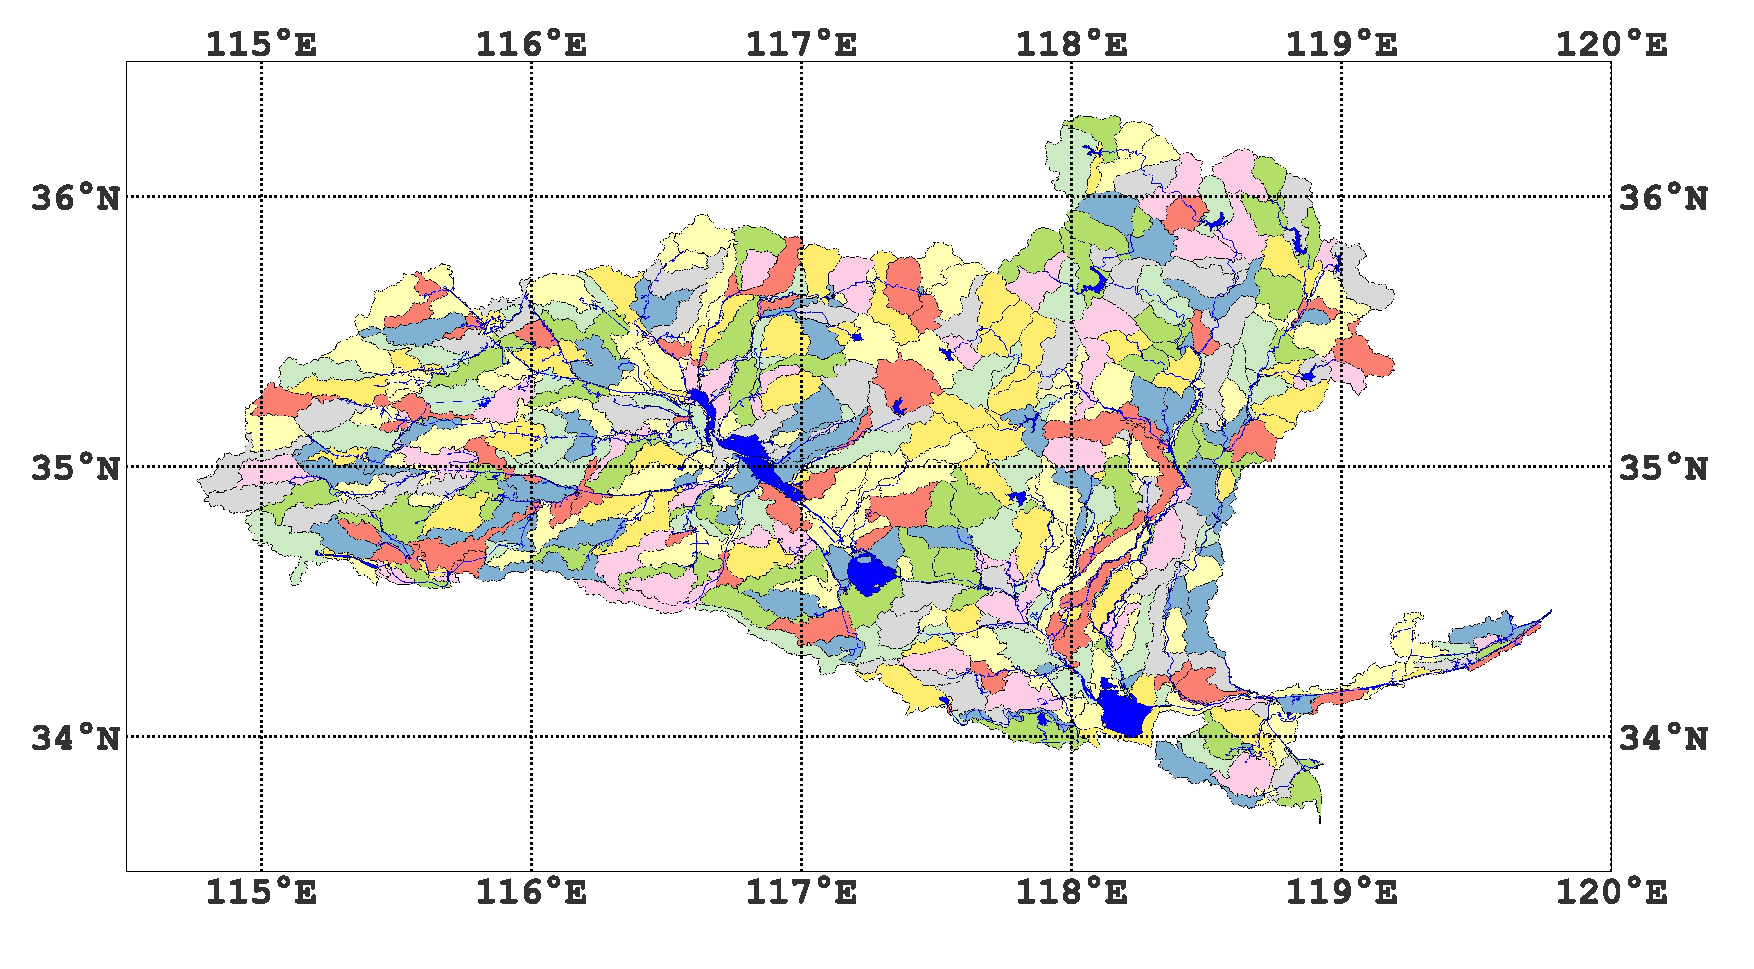
\includegraphics[width=\textwidth]{figures/CatchmentMesh_Huaihe.pdf}
    \caption{基于流域单元网格对淮河流域进行模拟时的流域单元划分图。本实例中,流域单元的面积阈值为250~$\mathrm{km^2}$。图中蓝色部分表示湖泊和河道,其余颜色代表流域单元。}
    \label{fig:fig_huaihe}
\end{figure}

define.h文件的内容为,
\lstinputlisting[language=fortran, basicstyle=\linespread{1.0}\footnotesize\ttfamily, commentstyle=\color{olive}, numbers=left, numberstyle=\tiny, xleftmargin=1.5em,xrightmargin=0em, aboveskip=1em]{examples/catchment/define.h}

Namelist文件的内容为,
\lstinputlisting[language=fortran, basicstyle=\linespread{1.0}\footnotesize\ttfamily, commentstyle=\color{olive}, numbers=left, numberstyle=\tiny, xleftmargin=1.5em,xrightmargin=0em, aboveskip=1em]{examples/catchment/HuaiRiver_Catch_250km2_IGBP_VG.nml}

此实例中,\par
1)区域大致范围通过DEF\_domain进行设定;\par
2)从文件DEF\_CatchmentMesh\_data中的'icatchment2d'变量读入\textbf{描述单元划分的数据};\par
3)文件DEF\_ElementNeighbour\_file中的数据描述了\textbf{侧向流模拟}所需的流域单元及单元之间的参数信息;\par
4)\textbf{并行化}方面,将全球分为5\textdegree$\times$ 5\textdegree 的数据块进行并行模拟(DEF\_nx\_blocks和DEF\_ny\_blocks),每24个进程为一个工作组(DEF\_PIO\_groupsize);\par
5)\textbf{地表覆盖类型数据}使用了2005年的数据(DEF\_LC\_YEAR);\par
6)\textbf{叶面积指数数据}使用了2005年的月数据(不随年份变化时,叶面积指数数据的年份同DEF\_LC\_YEAR),不随年份变化(DEF\_LAI\_CHANGE\_YEARLY);\par
7)使用FIT算法进行\textbf{土壤水热参数升尺度}(DEF\_USE\_SOILPAR\_UPS\_FIT);\par
8)使用冷启动的方式对土壤和积雪的状态进行\textbf{初始化}(DEF\_USE\_SoilInit和DEF\_USE\_SnowInit);\par
9)使用水体深度动态变化方案(DEF\_USE\_Dynamic\_Lake),其余\textbf{过程参数化方案}均使用模式默认值;\par
10)使用CRUJRA数据作为\textbf{大气驱动}(DEF\_forcing\_namelist);\par
11)每月保存一次\textbf{重启动}变量(DEF\_WRST\_FREQ);\par
12)\textbf{历史数据的输出},
\begin{itemize}[nosep,leftmargin=4em]
    \item 输出到0.05\textdegree 经纬度网格(DEF\_hist\_lon\_res和DEF\_hist\_lon\_res);
    \item 输出变量的日值(DEF\_HIST\_FREQ);
    \item 每月的数据保存在一个文件中(DEF\_HIST\_groupby);
    \item 输出所有变量(DEF\_hist\_vars\_out\_default).
\end{itemize}\par
13)其他配置使用模式默认值。


\section{实例7:非结构网格单元模拟}

本节配置了一个基于非结构网格单元的实例。实例使用了非结构网格单元,基于地表覆盖类型(IGBP)的植被结构次网格,以及van Genuchten-Mualem土壤水特征曲线模型,并基于MPI进行并行加速。

define.h文件的内容为,
\lstinputlisting[language=fortran, basicstyle=\linespread{1.0}\footnotesize\ttfamily, commentstyle=\color{olive}, numbers=left, numberstyle=\tiny, xleftmargin=1.5em,xrightmargin=0em, aboveskip=1em]{examples/unstructured/define.h}

Namelist文件的内容为,
\lstinputlisting[language=fortran, basicstyle=\linespread{1.0}\footnotesize\ttfamily, commentstyle=\color{olive}, numbers=left, numberstyle=\tiny, xleftmargin=1.5em,xrightmargin=0em, aboveskip=1em]{examples/unstructured/Tibet_unstructured_200km_IGBP_VG.nml}

此实例中,\par
1)区域大致范围通过DEF\_domain进行设定;\par
2)从文件DEF\_file\_mesh中的'elmindex'变量读入\textbf{描述单元划分的数据};\par
3)\textbf{并行化}方面,将全球分为5\textdegree$\times$ 5\textdegree 的数据块进行并行模拟(DEF\_nx\_blocks和DEF\_ny\_blocks),每24个进程为一个工作组(DEF\_PIO\_groupsize);\par
5)\textbf{地表覆盖类型数据}使用了2005年的数据(DEF\_LC\_YEAR);\par
6)\textbf{叶面积指数数据}使用了2005年的月数据(不随年份变化时,叶面积指数数据的年份同DEF\_LC\_YEAR),不随年份变化(DEF\_LAI\_CHANGE\_YEARLY);\par
7)使用FIT算法进行\textbf{土壤水热参数升尺度}(DEF\_USE\_SOILPAR\_UPS\_FIT);\par
8)使用热启动的方式对土壤状态进行\textbf{初始化}(DEF\_USE\_SoilInit),初始状态从文件DEF\_file\_SoilInit中读入;\par
9)使用冷启动的方式对积雪的状态进行\textbf{初始化}(DEF\_USE\_SnowInit);\par
10)使用ERA5数据作为\textbf{大气驱动}(DEF\_forcing\_namelist);\par
11)每月保存一次\textbf{重启动}变量(DEF\_WRST\_FREQ);\par
12)\textbf{历史数据的输出},
\begin{itemize}[nosep,leftmargin=4em]
    \item 输出到0.25\textdegree 经纬度网格(DEF\_hist\_lon\_res和DEF\_hist\_lon\_res);
    \item 输出变量的月值(DEF\_HIST\_FREQ);
    \item 每月的数据保存在一个文件中(DEF\_HIST\_groupby);
    \item 输出所有变量(DEF\_hist\_vars\_out\_default).
\end{itemize}\par
13)其他配置使用模式默认值。

\section{辅助工具包}
CoLM2024的辅助工具包包括案例创建、案例复制、案例代码比较、创建配置文件、案例代码更新和拷贝代码6个命令组成,这6个命令互相调用,集成不同的功能脚本。create\_newcase和create\_clone是两个案例创建功能脚本,create\_namelist,create\_script、create\_header和copy\_code是四个基础脚本,用于辅助案例创建的。update\_casecode用于版本控制后的案例代码更新。diff\_casecode用于比较两个案例之间,案例和主代码之间的差异。辅助工具包主要是基于案例的概念进行打造的,每个案例拥有独立案例目录,案例目录下包括独立的代码和配置,也就是说对于案例代码的修改,将不会影响其他案例和主代码,这大大地方便模式开发者对于版本的灵活控制。

\subsection{案例目录的结构}
\subsubsection{案例目录的结构}
执行辅助工具包将自动生成案例目录,案例目录由若干子目录和文件组成,包括代码目录(bld),运行脚本(mksrf.submit, init.submit和case.submit),模拟配置文件(namelist文件),历史文件目录(history$\slash$),重启文件目录(restart$\slash$)和地表数据目录(landdata$\slash$)。其中,代码目录包括源代码目录(bld$\slash$main$\slash$, bld$\slash$mkinidata$\slash$, bld$\slash$mksrfdata$\slash$和bld$\slash$share$\slash$,编译配置文件(bld$\slash$include$\slash$Makeoption)和宏配置文件(bld$\slash$include$\slash$define.h)。历史文件(见章节~\ref{history})、重启文件(见章节~\ref{restart})、地表数据(见章节~\ref{landdata})、namelist文件(见章节~\ref{nml})和宏配置文件(见章节~\ref{define.hux6587ux4ef6})的功能和可选项已在前面章节中详细介绍。代码目录和运行脚本是辅助运行工具包中的新内容。运行脚本用于队列系统的任务提交(如SLURM、LSF和QBS等队列系统),代码目录独立于主目录的代码,可以用于案例的代码修改和初期调试,宏配置文件也在该目录下。修改该目录下的代码或宏文件之后,可以直接编译并单独应用于该案例。

\subsection{辅助工具包的配置}

辅助工具包在移植到新机器使用前需要先编辑机器配置文件和队列系统脚本格式文件,配置并指定数据代码的路径、三个脚本运行需要的核数等机器信息和队列系统脚本格式。机器配置文件包含了新建案例所需的机器信息和数据路径信息(run$\slash$machine.config)见~\ref{table_machineconfig}。

\begin{table}[!htbp]
\caption{机器配置文件变量一览} \label{table_machineconfig}
\centering \renewcommand{\arraystretch}{1.2}
\begin{tabular}{lcp{0.35\textwidth}}
\toprule
\textbf{变量名} & \textbf{示例} & \textbf{说明} \\ \midrule
NProcesses\_mksrf & 672 & mksrf.submit脚本需要的核数 \\
NNodes\_mksrf & 14 & mksrf.submit需要的节点数目 \\
NTasksPerNode\_mksrf & 48 & mksrf.submit单节点核数 \\
Memory\_mksrf & 150G & mksrf.submit运行所申请内存 \\
Walltime\_mksrf & 24:00:00 & mksrf.submit运行所申请时间 \\
Queue\_mksrf & normal & mksrf.submit需要使用的队列 \\
NProcesses\_mkini & 48 &init.submit脚本需要的总核数 \\
NNodes\_mkini & 14 & init.submit需要的节点总数 \\
NTasksPerNode\_mkini & 48 & init.submit单节点核数 \\
Memory\_mkini & 150G & init.submit运行所申请内存 \\
Walltime\_mkini & 24:00:00 & init.submit运行所申请时间 \\
Queue\_mksrf & normal & init.submit需要使用的队列 \\
NProcesses\_case & 48 & case.submit脚本需要的核数 \\
NNodes\_case & 14 & case.submit需要的节点数目 \\
NTasksPerNode\_case & 48 & case.submit单节点核数 \\
Memory\_case & 150G & case.submit运行所申请内存 \\
Walltime\_case & 24:00:00 & case.submit运行所申请时间 \\
Queue\_mksrf & normal & case.submit需要使用的队列 \\
ROOT & \textasciitilde/CoLM/ & 代码个目录路径 \\
RAWDATA & \textasciitilde/rawdata/ & 模型所需的静态原始数据 \\
RUNTIME & \textasciitilde/runtime/ & 模型所需的动态地表数据 \\
MAKEOPTION & Makeoptions & 编译配置 (模板在include/下) \\
FORCINGPATH & \textasciitilde/GSWP3/ &气象驱动数据地址 \\
\bottomrule
\end{tabular} 
\end{table}

如须使用队列系统进行任务提交,需要通过编辑队列系统脚本格式文件来配置任务脚本的队列系统头信息格式(run$\slash$batch.config)。

\begin{lstlisting}
##run/batch.config
#------------------------------baiduboat-----------------------------
#!/bin/bash

#BSUB -J <CASENAME>
#BSUB -q <QUEUE>
#BSUB -o colm.o%
#BSUB -e colm.e%
#BSUB -n <NPROCESSES>
#BSUB -R rusage[mem=<MEMORY>]
#BSUB -R span[ptile=<NTASKSPERNODE>]
\end{lstlisting}

其中<CASENAME>是案例名,由案例创建命令create\_newcase收集(章节~\ref{CreateNewcase})。<QUEUE>、<NPROCESSES>、<MEMORY>和<NTASKSPERNODE>分别代表队列名、任务总核数、内存和单节点核数,由机器配置文件(run$\slash$machine.config)收集,见表~\ref{table_machineconfig}。冗余信息需要用\#注释掉。run$\slash$batch.config提供了SLURM、LSF和QBS的模板。

\subsection{案例创建脚本--create\_newcase} \label{CreateNewcase}
create\_newcase 将依照用户指定路径创建新的案例,允许用户按照典型案例配置或自定义案例进行配置的方法创建新的案例。其中包括创建namelist文件,创建运行脚本,创建头文件和代码拷贝,它们分别依赖create\_namelist、create\_script、create\_header和copy\_code四个基础脚本来实现。

创建新案例的方法有两种,典型配置创建案例和自定义配置创建案例。两种方法配置案例成功后,依然可以对案例namelist文件和宏定义define.h文件进行修改,手动修改或添加案例配置。

\subsubsection{典型配置创建案例}

典型配置创建案例语法较简单,适合初级用户快速展开模型运行。

语法:

\begin{lstlisting}
./create_newcase -n {案例运行路径} -c {典型案例配置选项名} [-t {起始年份}] [-e {结束年份}] [-f {气象驱动}]
\end{lstlisting}

案例运行路径为案例的绝对路径或相对路径,要求路径末尾没有"/"符号。典型案例配置选项目前包含5种(见表~\ref{tab:cases_config}),它分别包含了分辨率设置、次网格类型设置、生物地球化学开关和BGC半解析预热开关的设置。


例:
\begin{lstlisting}
./create_newcase -n ~/CoLM202X/cases/50km_PFT -c Global_Grid_50km_PFT_VG
\end{lstlisting}

\begin{table}[!htbp]
\renewcommand{\arraystretch}{1.5}
\centering 
\caption{典型案例配置一览}\label{tab:cases_config}
\begin{tabular}{
cccccc} \toprule
\textbf{典型案例配置选项名} & \textbf{分辨率} & \textbf{次网格} & \textbf{BGC} &\textbf{SASU}\\ \midrule
Global\_Grid\_50km\_PFT\_VG & 0.5$\times$0.5 & PFT & 关 &关\\
Global\_Grid\_50km\_USGS\_VG & 0.5$\times$0.5 & USGS & 关 &关\\
Global\_Grid\_50km\_PC\_VG & 0.5$\times$0.5 & PC & 关 & 关\\
Global\_Grid\_2x2\_PFT\_VG\_BGC & 2.5$\times$1.875 & PFT& 开 &关\\
Global\_Grid\_2x2\_PFT\_VG\_BGC-SASU & 2.5$\times$1.875 & PFT& 开 & 开\\
\bottomrule
\end{tabular}
\end{table}

所有典型案例为全球范围配置,如果未开启生物地球化学循环(BGC)时,默认分辨率为全球50km,开启BGC时,默认分辨率为全球2.5$\times$1.875分辨率。次网格包含植被功能型次网格(PFT),植物群落次网格(PC),地表覆盖类型次网格(LC),其中LC按不同数据来源包含了IGBP和USGS两种。SASU开启时,create\_newcase会自动帮助配置半解析加速预热方案(SASU),SASU仅在生物地球化学循环(BGC)开启时有效。

典型案例设置可以同时通过选项-t和-e设置运行起始和结束年份,通过-f选择气象驱动,通过-i设置预热的类型。时间、驱动和预热选项都是可缺失的,如果没有提供,起始和结束年份的默认值分别是1980年和2000年,气象驱动默认选择CRUJRA,预热选项默认关闭。


\subsubsection{自定义配置创建案例}

自定义配置创建案例通过手动配置模型起始时间、气象驱动、预热类型、格点类型(分辨率)、次网格类型、土壤水力参数模型、河道径流模型CaMa开关、生物地球化学模型开关、作物模型开关。其中,作物模型开关在生物地球化学模型开启时才生效;格点类型(分辨率)、次网格类型、土壤水力参数模型、河道径流模型CaMa开关、生物地球化学模型开关、作物模型开关在没有出现典型配置选项“-c”时才生效。

语法:
\begin{lstlisting}
./create_newcase -n {案例运行路径} [ -t {开始年份} ] [ -e {结束年份}] [ -f {气象驱动}] [ -g {格点类型} ] [ -s {次网格方案}] [ -m {土壤水力参数模型}] [ -r ] [-b [-p] [-i {预热方案}] ]  
\end{lstlisting}

案例运行路径为案例的绝对路径或相对路径,要求路径末尾没有"/"符号。自定义案例配置的详细配置见表~\ref{tab:custom_option}。所有自定义选项均为可缺失选项,缺省值见表~\ref{tab:custom_option}。

例:
\begin{lstlisting}
./create_newcase -n ~/CoLM202X/cases/50km_PFT -t 1980 -e 2000  -g grid_g144x96 -s PFT -m vg -b -i sasund 
\end{lstlisting}

\begin{table}[!htbp]
\renewcommand{\arraystretch}{1.5}
\centering 
\caption{自定义案例配置选项一览}\label{tab:custom_option}
\begin{tabular}{
cccccc} \toprule
\textbf{配置选项内容} & \textbf{配置选项} & \textbf{缺省值} & \textbf{备选值} & \textbf{有效条件}\\ \midrule
开始年份 & -t & 1980 & 任意整数 & 始终有效\\
结束年份 & -e & 2000 & 任意整数 & 始终有效\\
气象驱动 & -f & CRUJRA & CRUJRA; GSWP3  & 始终有效\\
格点类型 & -g & $\mathrm{grid}\_\mathrm{g}720\mathrm{x}360$ & 无& 无 -c\\
次网格方案 & -s & PFT & USGS; IGBP; PFT; PC & 无 -c\\
土壤水力模型 & -m & vg & vg; cb& 无 -c\\
Cama模型 & -r & 关 & 无& 无 -c\\
BGC模型 & -b & 关 & 无& 无 -c\\
作物模型 & -p & 关 & 无& 无 -c有 -b\\
预热方案 & -i & none & none; nd; sasund& 无 -c有 -b\\
\bottomrule
\end{tabular}
\end{table}

自定义案例配置选项按照有效条件可以任意组合,对新建案例进行配置,配置完成后,仍然可以通过文本编辑修改define.h, namelist以及三个任务提交脚本进行修改。

\subsection{案例复制脚本--create\_clone}

在方案比较实验中,经常需要运行两个配置相似的案例。使用案例复制命令create\_clone可以大大提高工作效率,并且降低配置出错的概率。

语法:
\begin{lstlisting}
./create_clone -s {待拷贝案例路径} -d {新案例路径}  
\end{lstlisting}

例:
\begin{lstlisting}
./create_clone -s ~/CoLM202X/cases/50km_PFT -d ~/CoLM202X/cases/50km_PFT-new  
\end{lstlisting}

待拷贝案例路径和新案例路径都要求路径末尾没有"/"符号。create\_clone语句将拷贝原案例的代码(bld目录)、运行脚本和namelist文件,并且识别案例名,对脚本和namelist中的案例名进行替换。

\subsection{案例的编译和运行}
\subsubsection{案例的编译}
对于案例代码的编译需要进入bld目录,并运行make命令。make前要确认编译配置文件(bld$\slash$include$\slash$Makeoption)的设置是否正确,包括netcfd库,Fortran编译器的选项和路径等(见章节~\ref{comprun})。

\subsubsection{案例目录的运行}
对于典型案例我们提供了适用于队列系统任务提交的三个脚本:地表数据制作任务提交脚本mksrf.submit,初始化任务提交脚本init.submit和模型运行任务提交脚本case.submit,他们分别对应章节~\ref{runcolm}中提到的三个colm运行步骤:地表数据制作、初始场数据制作和主程序运行。运行前需要检查队列系统所需要核数的设置是否和运行mpirun中要求的核数一致,其他内存和队列等配置是否符合服务器的要求。

\subsection{辅助工具包高级功能}

\subsubsection{案例代码的比较--diff\_casecode.bash}

在代码开发过程中,需要比较两个代码的差异,案例代码比较脚本可以帮助比较案例代码之间和案例代码与主代码的区别。

语法:

\begin{lstlisting}
./diff_casecode.bash {待比较案例1路径} [ {待比较案例2路径} ] 
\end{lstlisting}

例:
\begin{lstlisting}
./diff_casecode.bash ~/CoLM202X/cases/50km_PFT ~/CoLM202X/cases/50km_PFT-new1
或
./diff_casecode.bash  ~/CoLM202X/cases/50km_PFT
\end{lstlisting}

diff\_casecode.bash后可接两个参数或一个参数,参数指明案例路径,要求路径末尾没有"/"符号。当脚本命令后接两个参数并指定两个案例路径时,脚本将比较两个案例代码之间每行的差异。当脚本命令后接一个参数并制定一个案例路径时,脚本将比较该案例代码和主代码之间的差异,主代码路径需要通过编辑diff\_casecode.bash文件“ROOT=”行内容来指定。

\subsubsection{案例namelist文件的创建--create\_namelist}

模式运行的namelist文件可以通过create\_namelist脚本来创建。create\_namelist根据输入的开始结束年份、气象驱动、原始地表数据路径、运行数据路径、陆海分布数据、BGC预热方案和运行区域信息写入namelist文件。create\_namelist脚本所有选项一览表见表~\ref{tab:createnml_option}。

语法:
\begin{lstlisting}
./create_namelist {案例路径} {案例名} [-t {开始年份} ] [ -e {结束年份}] [ -f {气象驱动}] [ -d {原始地表数据路径}] [ -r {运行时数据路径}] [ -a {格点纬向分辨率} ] [ -o {格点经向分辨率} ] [ -S {区域南边界纬度} ] [ -N {区域北边界纬度} ] [ -E {区域东边界经度} ] [ -W {区域西边界经度} ] [ -i {BGC预热方案} ]
\end{lstlisting}

例:
\begin{lstlisting}
./create_namelist -p ~/CoLM202X/cases/ -n 50km_PFT -a 0.5 -o 0.5
\end{lstlisting}

\begin{table}[!htbp]
\renewcommand{\arraystretch}{1.5}
\centering 
\caption{create\_namelist配置选项一览}\label{tab:createnml_option}
\begin{tabular}{
cccccc} \toprule
\textbf{配置选项内容} & \textbf{配置选项} & \textbf{缺省值} & \textbf{备选值} & \textbf{有效条件}\\ \midrule
案例路径 & -p & 不可缺省 & 任意路径 & 始终有效 \\
案例名  & -n & 不可缺省 & 任意字符串 & 始终有效 \\
开始年份 & -t & 1980 & 任意整数 & 始终有效\\
结束年份 & -e & 2000 & 任意整数 & 始终有效\\
气象驱动 & -f & CRUJRA & CRUJRA; GSWP3  & 始终有效\\
原始地表数据路径 & -d & 无 & 任意路径 & 始终有效\\
运行数据路径 & -r & 无 & 任意路径 & 始终有效\\
经向分辨率 & -a & 0.5 & 任意数值 & 始终有效\\
纬向分辨率 & -o & 0.5 & 任意数值 & 始终有效\\
海陆分布数据路径 & -l & 无 & 任意路径 & 始终有效\\
区域南边界纬度 & -S & -90 & -90.0\textasciitilde90.0 小于北边界纬度 & 始终有效\\
区域北边界纬度 & -N & 90 & -90.0\textasciitilde90.0 大于南边界纬度 & 始终有效\\
区域西边界经度 & -S & -180 & -180.0\textasciitilde180.0 小于东边界经度 & 始终有效\\
区域东边界经度 & -N & 180 & -180.0\textasciitilde180.0 大于西边界经度 & 始终有效\\
BGC预热开关 & -i &none & none; nd; sasund& 始终有效 \\
\bottomrule
\end{tabular}
\end{table}

\subsubsection{案例脚本的创建--create\_script}

create\_script可以帮助用户生成可用于队列系统的三个任务脚本(mksrf.submit, init.submit和case.submit)。每个任务脚本根据batch.config和machine.config的内容来完成头信息的配置,它指定节点数目、CPU数目、内存使用和运行时间长度。create\_namelist脚本所有选项一览表见表~\ref{tab:createscript_option}。

create\_script根据BGC预热开关的设置(-i选项),为case.submit配置三种不同的预热方式:1) none, 2) nd, 3) sausund。BGC预热要求用脚本来控制单年驱动循环,1) none方式不包含BGC预热,可以用于非循环的模拟,为默认方案;2) nd方式为一年驱动循环的预热方式,case.submit中包含循环末尾对重启文件的重命名(时间戳的重命名),默认完成100次循环,可生脚本后通过手动编辑case.submit进行修改。3) sasund方式同为1年驱动循环的预热,case.submit中包含循环末尾对重启文件的重命名(时间戳重命名),默认完成130次循环,但前100次为半解析加速预热,后三十次为普通预热方式,类同于nd方式。

语法
\begin{lstlisting}
./create_scripts -p {案例路径} -t {开始年份} -e {结束年份} -f {batch配置文件路径} -c {机器配置文件路径} -i {BGC预热方案}
\end{lstlisting}

例:
\begin{lstlisting}
./create_scripts -p ~/CoLM202X/cases/50km_PFT -t 1850 -e 1850 -f ~/CoLM202X/run/batch.config -c ~/CoLM202X/run/machine.config -i nd
\end{lstlisting}

\begin{table}[!htbp]
\renewcommand{\arraystretch}{1.5}
\centering 
\caption{create\_script配置选项一览}\label{tab:createscript_option}
\begin{tabular}{
cccccc} \toprule
\textbf{配置选项内容} & \textbf{配置选项} & \textbf{缺省值} & \textbf{备选值} & \textbf{有效条件}\\ \midrule
案例路径名 & -p & 不可缺省 & 任意路径 & 始终有效 \\
开始年份 & -t & 不可缺省 & 任意整数 & 始终有效\\
结束年份 & -e & 不可缺省 & 任意整数 & 始终有效\\
batch配置文件路径 & -f & 不可缺省 & 任意路径 & 始终有效 \\
机器配置文件路径 & -f & 不可缺省 & 任意路径 & 始终有效 \\
BGC预热开关 & -i &none & none; nd; sasund& 始终有效 \\
\bottomrule
\end{tabular}
\end{table}

\subsubsection{案例代码更新--update\_casecode}

随着代码的发展,本地仓库会通过github进行更新。案例代码常常需要随着本地仓库代码的更新而更新。运用案例代码更新脚本可以帮助实现案例代码的更新。但需注意,案例代码更新脚本仅仅实现拷贝覆盖代码的功能,尚无法实现代码合并(merge)的功能。因此,更新代码前须妥善处理案例代码已更新的部分。注意:在使用前,需要编辑update\_casecode中的ROOT变量,定位本地仓库代码。

语法:
\begin{lstlisting}
./update_casecode {待更新的案例路径}
\end{lstlisting}
另外,确保待更新的案例路径后没有"/"。

例:
\begin{lstlisting}
./update_casecode ~/CoLM202X/cases/50km_PFT
\end{lstlisting}


\subsubsection{案例代码复制--copy\_code}
copy\_code将原案例或本地仓库代码拷贝到新案例代码路径,是案例复制脚本(create\_clone)和案例代码更新脚本(update\_casecode)的一部分。相比create\_clone,copy\_code的差异在于它仅拷贝代码不操作namelist和任务脚本文件。注意:案例代码路径需要给到案例的bld目录地址,本地仓库代码路径给到本地仓库地址即可。

语法:
\begin{lstlisting}
./copy_code -s {待复制代码路径} -d {目标代码路径} 
\end{lstlisting}

例:
\begin{lstlisting}
./copy_code -s ~/CoLM202X/cases/50km_PFT/bld -d ~/CoLM202X/cases/50km_PFT-new1/bld
或
./copy_code -s ~/CoLM202X -d ~/CoLM202X/cases/50km_PFT-new1/bld
\end{lstlisting}
第二个例子等同于用update\_casecode更新案例50km\_PFT-new1

\clearpage

\part{研发用户指南}

\section{通用陆面模式中的自定义数据类型}

\subsection{格点数据}
CoLM中使用的地表覆盖类型、土壤属性、叶面积指数、流域划分、湖泊深度和树高等细分辨率数据,以及大气驱动和历史输出等粗分辨率数据都是格点数据。

为了处理高分辨率数据和进行并行计算,CoLM对所有格点数据进行分块。分块方案为:通过设置Namelist文件中的DEF\_nx\_blocks和DEF\_ny\_blocks两个变量的值,将经向180\textdegree W至180\textdegree E等分为DEF\_nx\_blocks段,将纬向90\textdegree N至90\textdegree S等分为DEF\_ny\_blocks段。对区域模拟,同样指的是对全球进行分块。格点数据分块进行读取和使用,以双精度浮点型数据为例,在代码(share/MOD\_DataType.F90)中“格点数据”的自定义数据类型为
\begin{lstlisting}[language=fortran, basicstyle=\linespread{1.0}\footnotesize\ttfamily, commentstyle=\color{olive}, numbers=left, numberstyle=\tiny, xleftmargin=1.5em,xrightmargin=0em, aboveskip=1em]
   type :: pointer_real8_2d
      real(r8), allocatable :: val (:,:)
   CONTAINS
      final :: pointer_real8_2d_free_mem
   END type pointer_real8_2d

   type :: block_data_real8_2d
      type(pointer_real8_2d), allocatable :: blk (:,:)
   CONTAINS
      final :: block_data_real8_2d_free_mem
   END type block_data_real8_2d
\end{lstlisting}
此外,代码中还定义了整型格点数据以及三维、四维格点数据。

格点数据建立在固定的经纬度网格上,经纬度网格在CoLM中使用自定义数据结构“网格”进行描述。网格数据结构包含了每个数据块的经纬度信息、全局位置、数据大小以及其他辅助信息。以下代码展示了如何在网格grid上建立双精度浮点型格点数据gdata2d,
\begin{lstlisting}[language=fortran, basicstyle=\linespread{1.0}\footnotesize\ttfamily, commentstyle=\color{olive}, numbers=left, numberstyle=\tiny, xleftmargin=1.5em,xrightmargin=0em, aboveskip=1em]
    type(grid_type),           intent(in)  :: grid
    type(block_data_real8_2d), intent(out) :: gdata2d

    ! 在网格grid上建立双精度浮点型格点数据gdata2d
    CALL allocate_block_data (grid, gdata2d)
\end{lstlisting}
模式中对格点数据类型定义了析构函数,因此,使用格点数据的代码结束时,无需编写释放内存的代码。

从netCDF文件中读取格点数据可使用以下函数(其中filename和dataname分别为文件名和文件中的变量名),
\begin{lstlisting}[language=fortran, basicstyle=\linespread{1.0}\footnotesize\ttfamily, commentstyle=\color{olive}, numbers=left, numberstyle=\tiny, xleftmargin=1.5em,xrightmargin=0em, aboveskip=1em]
   CALL ncio_read_block (filename, dataname, grid, gdata2d)
\end{lstlisting}

若netCDF文件中的数据包含时间维度,可使用以下函数(其中itime为文件中时间维度的值),
\begin{lstlisting}[language=fortran, basicstyle=\linespread{1.0}\footnotesize\ttfamily, commentstyle=\color{olive}, numbers=left, numberstyle=\tiny, xleftmargin=1.5em,xrightmargin=0em, aboveskip=1em]
   CALL ncio_read_block_time (filename, dataname, grid, itime, gdata2d)
\end{lstlisting}

以上函数allocate\_block\_data, ncio\_read\_block, ncio\_read\_block\_time对整型、浮点型以及二维、三维数据做了重载,因此,使用时函数名中未加数据类型及维数。

对格点数据的定位需要同时使用分块信息和网格信息,以下代码展示了如何对格点数据进行操作,
\begin{lstlisting}[language=fortran, basicstyle=\linespread{1.0}\footnotesize\ttfamily, commentstyle=\color{olive}, numbers=left, numberstyle=\tiny, xleftmargin=1.5em,xrightmargin=0em, aboveskip=1em]
    IF (p_is_io) THEN
        DO iblkme = 1, gblock%nblkme
            ib = gblock%xblkme(iblkme)
            jb = gblock%yblkme(iblkme)

            DO j = 1, grid%ycnt(jb)
                DO i = 1, grid%xcnt(ib)
                    ! 对gdata2d%blk(ib,jb)%val(i,j)进行操作
                ENDDO
            ENDDO
        ENDDO
    ENDIF
\end{lstlisting}
这段代码中,首先判断本进程是否为IO进程(格点数据仅位于读写进程的内存中,见第\ref{ch_parallel}节)。若是,则从gblock变量中循环获取分配给本进程的数据块的位置(代码中的ib和jb)。对分配给本进程的每个数据块,可进一步通过循环(代码中的j和i),对每个网格点上的数据进行操作。

\subsection{向量数据}

CoLM中的斑块(patch)、流域单元、非结构网格单元、水文响应单元、植被功能类型单元和植物群落单元等都具有不规则的形状,这些不规则形状单元在模式中使用细分辨率格点的集合进行表示。例如,使用0.5\textdegree 度经纬度网格单元进行陆面过程模拟时,在单元内部使用500米分辨率的地表覆盖类型数据建立次网格斑块单元,此时,一个斑块单元表示在一个0.5\textdegree 网格内部具有相同地表覆盖类型的500米细分辨率格点的集合。又如,使用流域单元进行陆面过程模拟时,根据90米高分辨率的水文学数据对模拟区域进行流域单元的划分,一个流域单元在模式中表示为90米细分辨率的格点的集合。

定义在不规则形状单元上的变量在模式中使用“向量”数据结构,为一维、二维或者三维数组,数组的最后一个维度的长度等于不规则单元的数量。例如定义在斑块上的叶面积指数
\begin{lstlisting}[language=fortran, basicstyle=\linespread{1.0}\footnotesize\ttfamily, commentstyle=\color{olive}, numbers=left, numberstyle=\tiny, xleftmargin=1.5em,xrightmargin=0em, aboveskip=1em]
    IF (p_is_worker) THEN
       allocate (lai (numpatch))
    ENDIF
\end{lstlisting}
这段代码中,首先判断本进程是否为worker进程(向量数据仅位于工作进程的内存中,见第\ref{ch_parallel}节)。若是,则定义一个一维数组存储叶面积指数的值,其长度等于分配到本进程的斑块的数量(numpatch)。

\subsection{格点数据和向量数据之间的映射}

陆面模式的输入数据(地表数据、大气驱动数据等)多为格点数据,而模式的基本单元为斑块等不规则单元,因此,需将格点数据映射到网格数据。CoLM中主要使用两种将格点数据映射到向量数据的方法,一种是面积加权平均,另一种是双线性插值。

以下代码定义和构建了由格点数据向斑块单元的面积加权平均映射,
\begin{lstlisting}[language=fortran, basicstyle=\linespread{1.0}\footnotesize\ttfamily, commentstyle=\color{olive}, numbers=left, numberstyle=\tiny, xleftmargin=1.5em,xrightmargin=0em, aboveskip=1em]
    type (grid_type) :: gforc
    type (pixelset_type) :: landpatch
    type (spatial_mapping_type) :: mg2p_forc
    
    ! 构建由定义在网格gforc上的格点数据向斑块单元的面积加权平均映射
    CALL mg2p_forc%build_arealweighted (gforc, landpatch)    
\end{lstlisting}
具体实现时,面积加权平均方法先将格点数据映射到不规则单元内的细网格上,再对细网格进行加权平均,其可保证在映射的过程中变量是守恒的。上述映射只需在初始化时构建一次,调用以下函数进行使用
\begin{lstlisting}[language=fortran, basicstyle=\linespread{1.0}\footnotesize\ttfamily, commentstyle=\color{olive}, numbers=left, numberstyle=\tiny, xleftmargin=1.5em,xrightmargin=0em, aboveskip=1em]
    CALL mg2p_forc%grid2pset (forc_xy_t, forc_t) 
\end{lstlisting}
其中,forc\_xy\_t为格点数据,forc\_t为向量数据。

以下代码定义和构建了由格点数据向斑块单元的双线性插值映射,
\begin{lstlisting}[language=fortran, basicstyle=\linespread{1.0}\footnotesize\ttfamily, commentstyle=\color{olive}, numbers=left, numberstyle=\tiny, xleftmargin=1.5em,xrightmargin=0em, aboveskip=1em]
    type (grid_type) :: gforc
    type (pixelset_type) :: landpatch
    type (spatial_mapping_type) :: mg2p_forc
    
    ! 构建由定义在网格gforc上的格点数据向斑块单元的双线性插值映射
    CALL mg2p_forc%build_bilinear (gforc, landpatch)    
\end{lstlisting}
具体实现时,双线性映射方法将格点数据视为定义在经纬度网格点的中心位置,向量数据视为定义在不规则单元的重心位置,由包围不规则单元重心点的四个网格中心点向不规则单元进行插值。单独的双线性映射方法不能保证变量的守恒性,但与面积加权平均方法相比,使得插值后的变量在空间上较为平滑。上述映射同样只需在初始化时构建一次,调用以下函数进行使用
\begin{lstlisting}[language=fortran, basicstyle=\linespread{1.0}\footnotesize\ttfamily, commentstyle=\color{olive}, numbers=left, numberstyle=\tiny, xleftmargin=1.5em,xrightmargin=0em, aboveskip=1em]
    CALL mg2p_forc%grid2pset (forc_xy_t, forc_t) 
\end{lstlisting}
其中,forc\_xy\_t为格点数据,forc\_t为向量数据。

模式结果通常以格点数据的方式输出,以增强可视化和结果分析的便利性,因此,需在输出时将定义在基本模拟单元上的向量数据映射到格点数据。向量数据向格点数据映射的构建与上述格点数据向向量数据映射的构建是相同的,使用时,以下函数
\begin{lstlisting}[language=fortran, basicstyle=\linespread{1.0}\footnotesize\ttfamily, commentstyle=\color{olive}, numbers=left, numberstyle=\tiny, xleftmargin=1.5em,xrightmargin=0em, aboveskip=1em]
    CALL mp2g_hist%pset2grid (hist_t, hist_xy_t, spv = filledvalue, msk = filter) 
\end{lstlisting}
执行向量数据hist\_t向格点数据hist\_xy\_t的映射,其中spv和msk为两个可选参数。浮点数spv表示计算过程中不予考虑的填充值。msk为逻辑型向量数据,其第i个元素值为TRUE时表示此不规则单元参与映射,值为FALSE时表示不参与映射。例如,在输出湖泊温度时,可使用msk变量,将所有湖泊单元表示出来进行映射和输出。值得注意的是,当从向量数据向格点数据进行映射时,执行函数mp2g\_hist\%pset2grid得到的结果hist\_xy\_t表示格点内变量的总量,若要计算变量的均值,可先执行
\begin{lstlisting}[language=fortran, basicstyle=\linespread{1.0}\footnotesize\ttfamily, commentstyle=\color{olive}, numbers=left, numberstyle=\tiny, xleftmargin=1.5em,xrightmargin=0em, aboveskip=1em]
    CALL mp2g_hist%get_sumarea (sumarea, filter)
\end{lstlisting}
得到格点内参与映射的不规则单元的总面积sumarea,然后在每个格点内用变量的总量除以总面积得到均值。


\section{并行计算构架}\label{ch_parallel}

CoLM 2024版使用MPI(Massage Passing Interface)函数库实现在多核小型机、服务器以及超级计算机上的并行计算。

当使用多个进程运行模式时,所有进程被分为四类(见图~\ref{fig:fig_parallelization}),分别为主进程、读写进程、工作进程和回写进程。主进程(master)处理全局的输入输出和在运行过程中打印信息。读写进程(IO)进行数据的分发、收集和读写。工作进程(worker)执行模式过程。回写进程为可选项,专门用于历史文件的写出。一个工作组由一个读写进程和多个工作进程组成。

\begin{figure}[htpb]
    \centering
    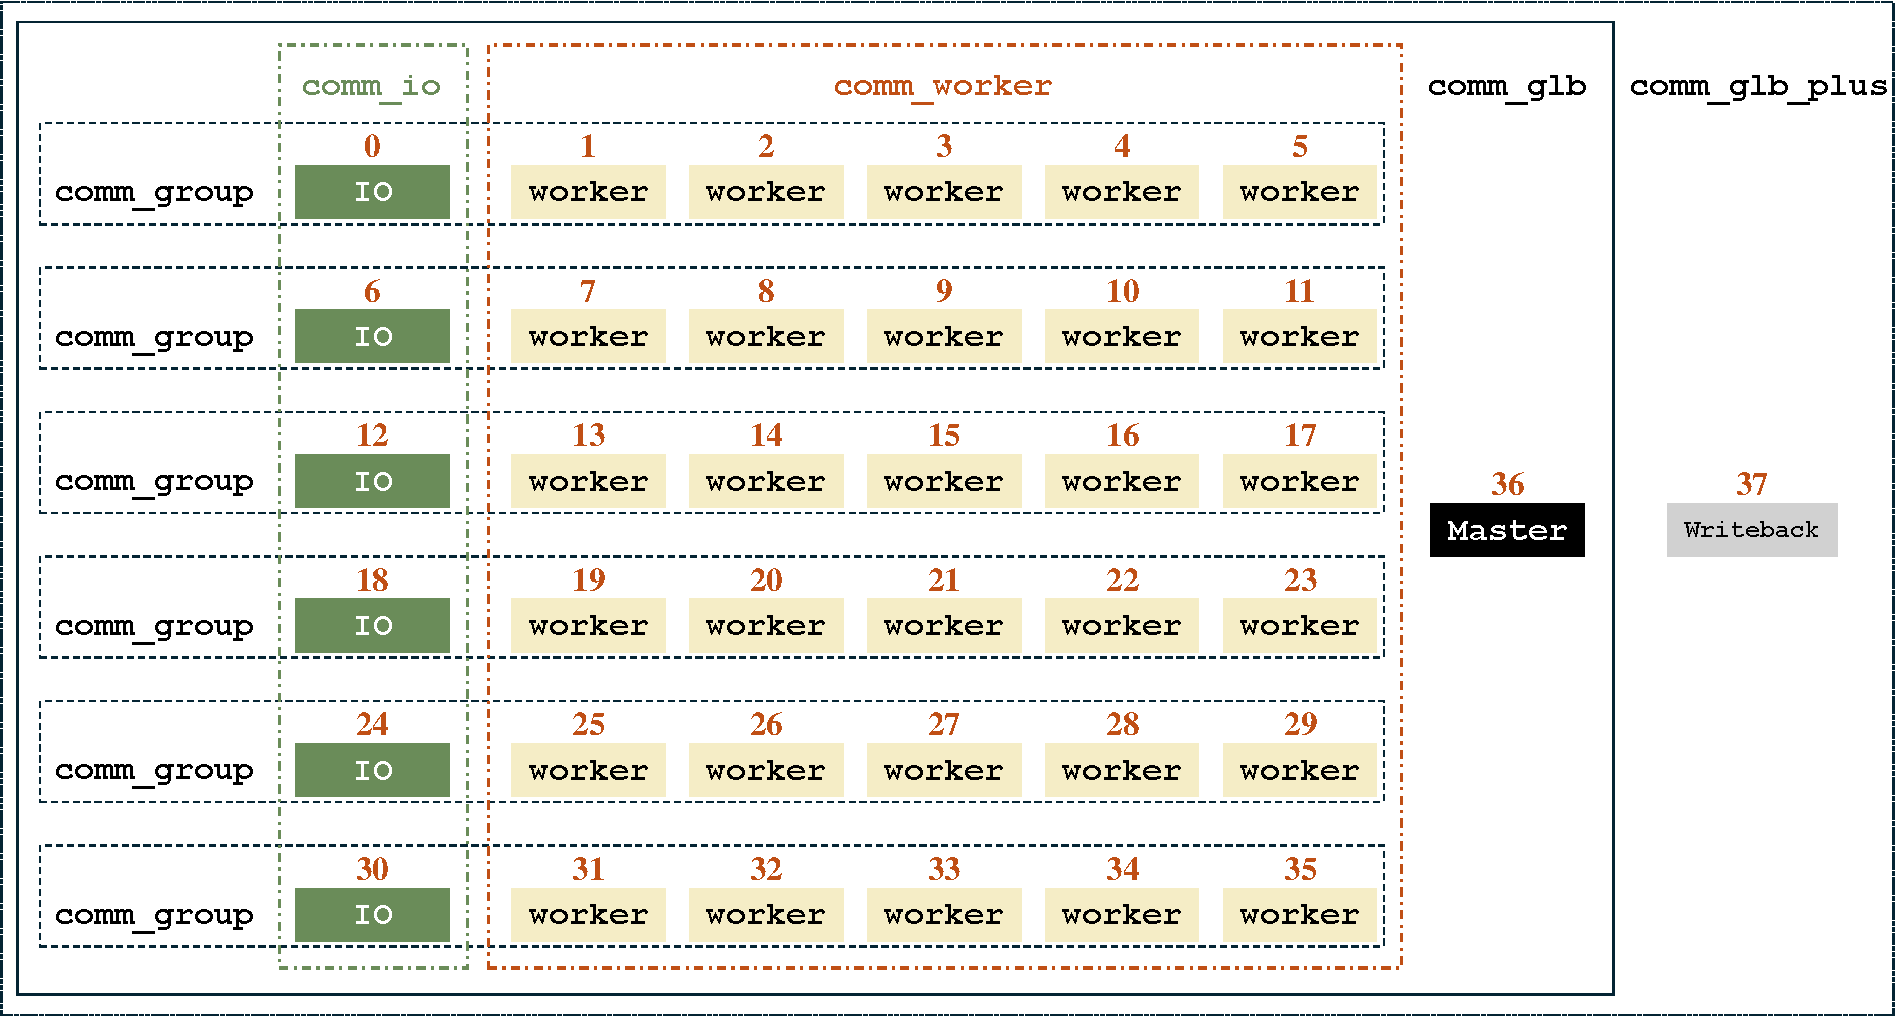
\includegraphics[width=\textwidth]{figures/并行计算图.pdf}
    \caption{CoLM 2024版并行计算构架示意图。其中所有进程被分为四类,分别为主进程、读写进程、工作进程和回写进程,数字标号0\textasciitilde 37为进程的全局编号。comm\_group为一个读写进程和多个工作进程组成的工作组通讯域,comm\_io为所有读写进程组成的通讯域,comm\_worker为所有工作进程组成的通讯域,comm\_glb为主进程、读写进程和工作进程组成的通讯域,comm\_glb\_plus为所有进程的通讯域。}
    \label{fig:fig_parallelization}
\end{figure}

并行运行模式时,模式以加权轮询的方式将数据块分配到工作组(见图~\ref{fig:fig_block}),每个工作组主要负责其分配到的数据块上的读写和模式计算。在工作组内,工作任务的分配以陆表单元(Element)为基本单位,每个陆表单元内部进一步划分的水文响应单元(HRU)、次网格单元(patch)、植被功能类型单元(PFT)以及植被群落单元(PC)等都分配到同一个进程上。工作组内任务的分配方法为将每个数据块上的陆表单元均匀分配,例如,某数据块有150个陆表单元,负责其计算的工作组有4个工作进程,将陆表单元按编号排序后,第1到4个工作进程分别进行第1到38、第39到76,第77到113,第114到150个陆表单元上的模拟。

\begin{figure}[htpb]
    \centering
    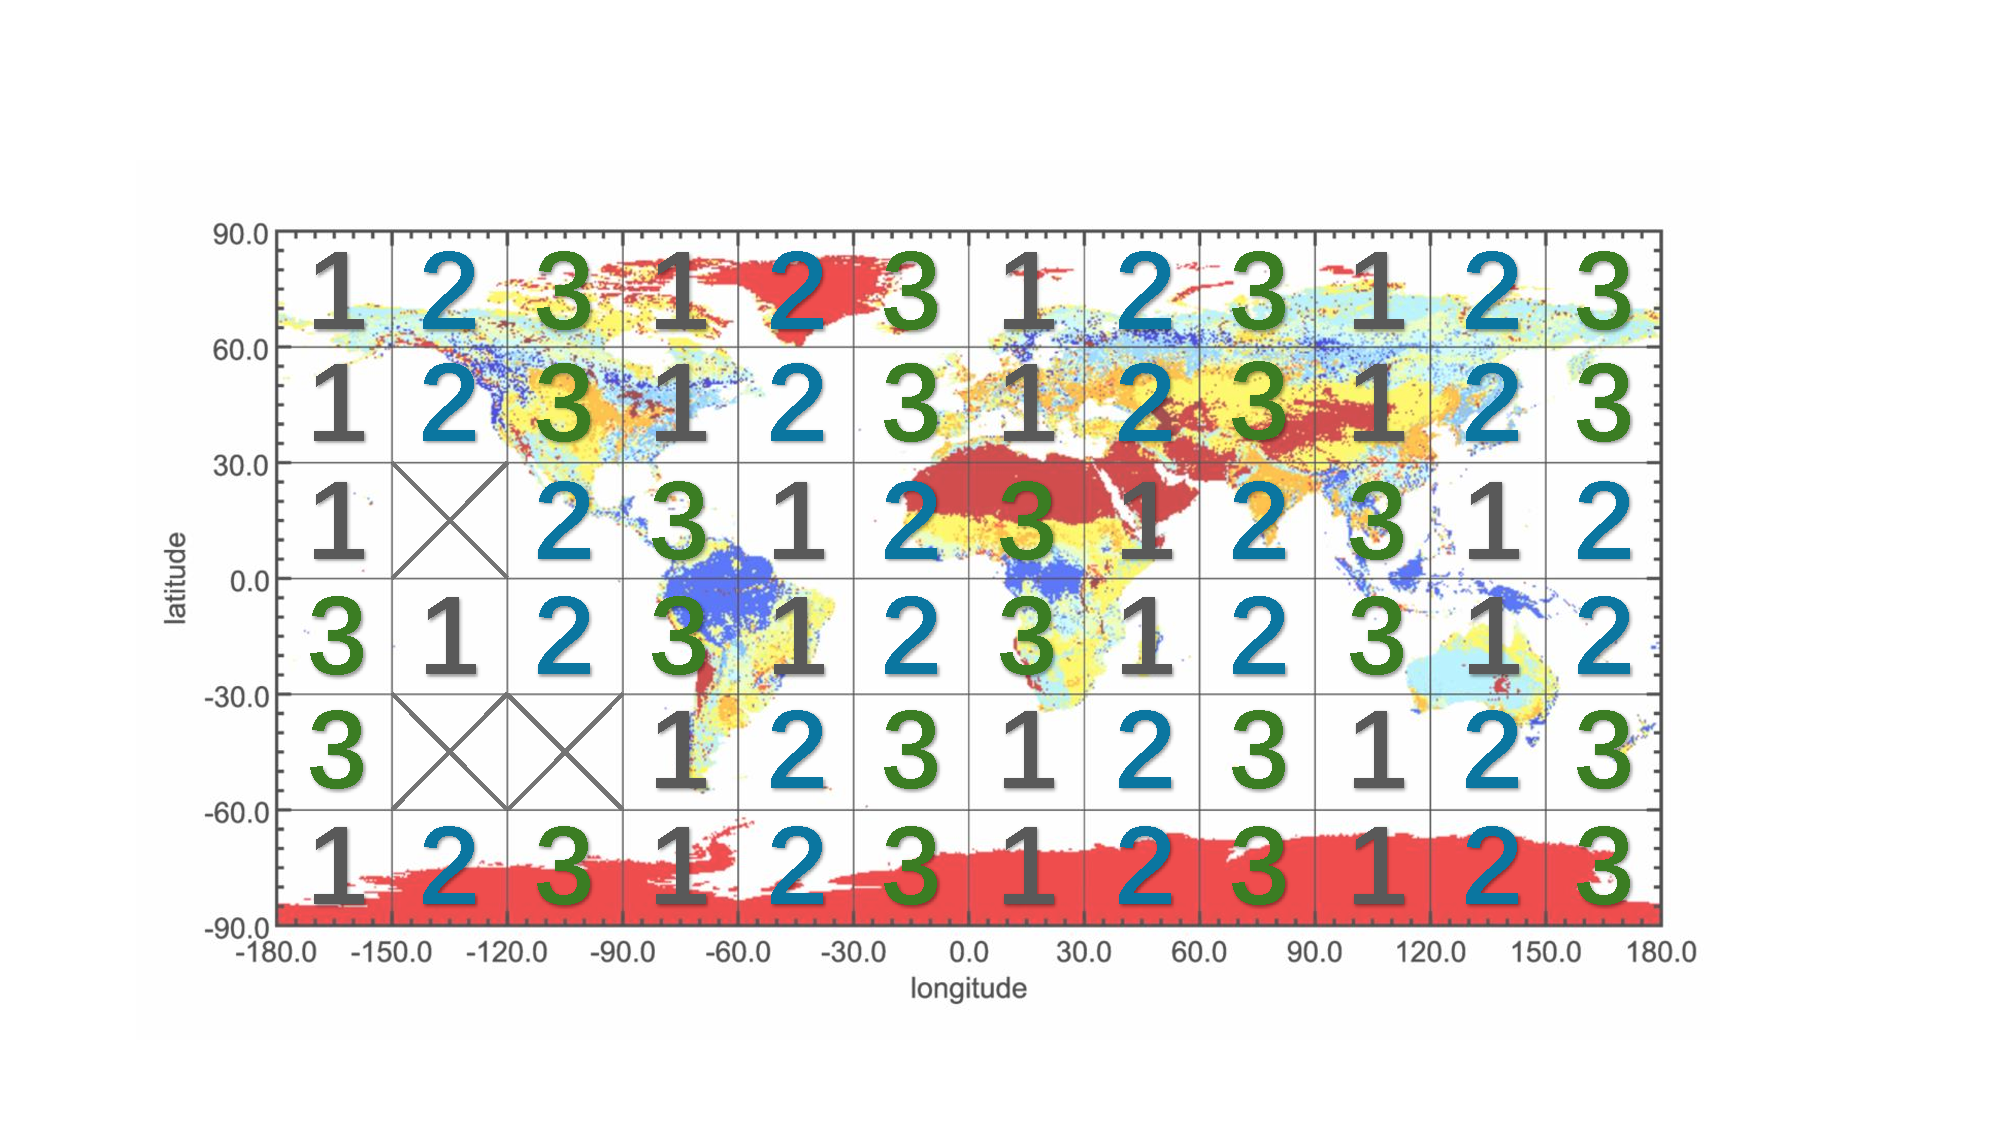
\includegraphics[width=\textwidth]{figures/数据分块示意图.pdf}
    \caption{CoLM 2024版数据分块及并行任务分配示意图。本例中将全球分为30\textdegree$\times$ 30\textdegree 的数据块。当使用3个工作组运行模式时,数据分块以轮询的方式分配到工作组,图中的数字1,2,3表示负责该数据块的工作组的编号。}
    \label{fig:fig_block}
\end{figure}

格点数据主要储存在读写进程(IO)的内存中,其读写有多种方式,可适应不同的计算环境。读入格点数据时,每个读写进程直接从外部文件中读入其负责的数据块上的数据。向外部文件写入格点数据有三种方式。第一种方式,当DEF\_HIST\_mode为'block'时,读写进程将每个数据块的内容写入单独的文件,这种方式通常具有最高的写文件速度,但分析结果时需要后处理程序拼接数据。第二种方式,当DEF\_HIST\_mode为'one'且DEF\_HIST\_WriteBack为FALSE时,由主进程在运行过程中从读写进程收集所有数据块的数据,进行拼接后将完整数据写出,这种方式不需要进行后期数据处理,但因收集数据时使用了阻塞通讯,在数据量较大时效率低、耗时长。第三种方式,当DEF\_HIST\_mode为'one'且DEF\_HIST\_WriteBack为TRUE时,模式将全局编号最大的进程独立出来作为回写进程,回写进程在运行过程中从读写进程收集所有数据块的数据,进行拼接后将完整数据写出,与第二种方式不同的是,读写进程向回写进程发送数据块上的数据时,使用的是非阻塞通讯,可不等待数据接收完成就继续向下运行。

向量数据主要储存在工作进程(worker)的内存中,其读写需通过读写进程(IO)。从外部文件读取向量数据时,读写进程首先读入其负责的数据块上的向量数据的子集,再分发给其工作组中的工作进程,分发过程通过进程之间的通讯实现。当向外部文件写入向量数据时,读写进程首先通过进程之间的通讯从其工作组中的工作进程收集数据,再按数据块将数据写入独立的文件。

因格点数据和向量数据分别位于读写进程和工作进程的内存中,格点数据和向量数据之间的映射均需通过进程之间的通讯实现。离线模拟时,大气驱动数据通常为格点数据,由读写进程读入后,按需发送至工作进程,再映射到向量数据。以经纬度网格进行历史数据输出时,需从工作进程发送以向量数据为形式的模拟结果至读写进程,再由读写进程累加到格点上。这些数据收发和累加映射的函数已封装在模块MOD\_SpatialMapping中,一般不需要开发者自己改写代码。

% \section{网格的定义}

\end{document}
